\documentclass[10pt,titlepage]{article} % NORMALNA PRACA
\renewcommand{\normalsize}{\fontsize{8pt}{10pt}\selectfont} % DO ARCHIWUM

\usepackage{graphicx, wrapfig, lipsum}
%\usepackage{graphics}
\usepackage{xfrac}
\usepackage{subfig}
\usepackage{epsfig}
\usepackage{amsmath}
\usepackage{amssymb}
\usepackage{amsthm}
\usepackage{booktabs}
\usepackage{stmaryrd}
\usepackage{url}
\usepackage{enumerate}
\usepackage{tabu}
\usepackage[figuresright]{rotating}
\usepackage{titlesec}
\usepackage{hyperref} 
\usepackage{polski}
\usepackage[utf8]{inputenc}
\usepackage[T1]{fontenc}
\usepackage{geometry}
\usepackage{pslatex}
\usepackage{ulem}
\usepackage{caption}
\usepackage{listings}
\usepackage{url}
\usepackage{Here}
\usepackage{scrextend}
\usepackage{newfloat}
\usepackage{color}
\usepackage{harveyballs}
\definecolor{szary}{gray}{0.75}% jasnoszary

%\usepackage{filecontents}
%\usepackage{blindtext}
%\usepackage[nottoc,numbib]{tocbibind}

\lstset{numbers=left,
			numberstyle=\tiny, 
			basicstyle=\scriptsize\ttfamily, 
			breaklines=true, 
			captionpos=b, 
			tabsize=2}

\usepackage[ruled,vlined,linesnumbered]{algorithm2e}

\vfuzz2pt % Don't report over-full v-boxes if over-edge is small
\hfuzz2pt % Don't report over-full h-boxes if over-edge is small


\newcommand{\RR}{\mathbb{R}}
\newcommand{\NN}{\mathbb{N}}
\newcommand{\QQ}{\mathbb{Q}}
\newcommand{\ZZ}{\mathbb{Z}}
\newcommand{\TAB}{\hspace{0.50cm}}
\newcommand{\IFF}{\leftrightarrow}
\newcommand{\IMP}{\rightarrow}

\renewcommand*{\figurename}{Rys.} 
\renewcommand*{\tablename}{Tab.}

\newtheorem{theorem}{Twierdzenie}[section]
\newtheorem{lemma}{Lemat}[section]
\newtheorem{example}{Przykład}[section]
\newtheorem{corollary}{Wniosek}[section]
\newtheorem{definition}{Definicja}[section]

\hyphenation{wszy-stkich ko-lu-mnę każ-da od-leg-łość
   dzie-dzi-ny dzie-dzi-na rów-nych rów-ny
   pole-ga zmie-nna pa-ra-met-rów wzo-rem po-cho-dzi
   o-trzy-ma wte-dy wa-run-ko-wych lo-gicz-nie
   skreś-la-na skreś-la-ną cał-ko-wi-tych wzo-rów po-rzą-dek po-rząd-kiem
   przy-kład pod-zbio-rów po-mię-dzy re-pre-zen-to-wa-ne
   rów-no-waż-ne bi-blio-te-kach wy-pro-wa-dza ma-te-ria-łów
   prze-ka-za-nym skoń-czo-nym mo-żesz na-tu-ral-na cią-gu tab-li-cy
   prze-ka-za-nej}

\titleclass{\subsubsubsection}{straight}[\subsection]

\newcounter{subsubsubsection}[subsubsection]
\renewcommand\thesubsubsubsection{\thesubsubsection.\arabic{subsubsubsection}}
\renewcommand\theparagraph{\thesubsubsubsection.\arabic{paragraph}} % optional; useful if paragraphs are to be numbered

\titleformat{\subsubsubsection}
  {\normalfont\normalsize\bfseries}{\thesubsubsubsection}{1em}{}\titlespacing*{\subsubsubsection}
{0pt}{3.25ex plus 1ex minus .2ex}{1.5ex plus .2ex}

\makeatletter
\renewcommand\paragraph{\@startsection{paragraph}{5}{\z@}%
  {3.25ex \@plus1ex \@minus.2ex}%
  {-1em}%
  {\normalfont\normalsize\bfseries}}
\renewcommand\subparagraph{\@startsection{subparagraph}{6}{\parindent}%
  {3.25ex \@plus1ex \@minus .2ex}%
  {-1em}%
  {\normalfont\normalsize\bfseries}}
\def\toclevel@subsubsubsection{4}
\def\toclevel@paragraph{5}
\def\toclevel@paragraph{6}
\def\l@subsubsubsection{\@dottedtocline{4}{7em}{4em}}
\def\l@paragraph{\@dottedtocline{5}{10em}{5em}}
\def\l@subparagraph{\@dottedtocline{6}{14em}{6em}}
\makeatother

\setcounter{secnumdepth}{4}
\setcounter{tocdepth}{4}

\DeclareFloatingEnvironment[
  fileext=lop,
  listname={Spis listingów},
  %name=Plot,
  placement=tp,
  %within=section,% activate it if you want
  %chapterlistsgaps=on,% only meaningful when chapters exist
]{listing}


\begin{document}

\pagestyle{empty} %To jest strona tytułowa, bez numeracji

%\begin{titlepage}
%\vspace*{\fill}
%\begin{center}
%\begin{picture}(300,510)
%\put( 150,450){\makebox(0,200)[3]{\huge \bf \textsc{POLITECHNIKA WROCŁAWSKA }}}
%\put( 150,420){\makebox(0,200)[3]{\huge \bf \textsc{WYDZIAŁ ELEKTRONIKI }}}
%\put(-110,505){\noindent\rule{18cm}{0.4pt}}
%\put(-110,480){\makebox(0,0)[l]{\large     \textsc{KIERUNEK: INFORMATYKA}}}
%\put(-110,460){\makebox(0,0)[l]{\large     \textsc{SPECJALNOŚĆ: INŻYNIERIA SYSTEMÓW INFORMATYCZNYCH}}}
%\put( 120,330){\makebox(0,200)[3]{\huge \bf \textsc{PRACA DYPLOMOWA }}}
%\put( 150,310){\makebox(0,200)[3]{\huge \bf \textsc{INŻYNIERSKA }}}

%  \put( 150,280){\makebox(0,200)[3]{\Large \bf \textsc{Aplikacja internetowa wspomagająca aukcyjną }}}
%  \put( 150,240){\makebox(0,200)[4]{\Large \bf \textsc{organizację usług przewozu towarów }}}
%  \put(100,240){\makebox(0,0)[l]{\large     \textsc{Hubert Olkiewicz}}}

%  \put(100,-80){\makebox(0,0)[bl]{\large \bf \textsc{Wrocław 2016}}}
%\end{picture}
%\end{center}
%\vspace*{\fill}
%\end{titlepage}

\tableofcontents

\listoffigures
\listoflistings
\listoftables


\newpage
%\pagenumbering{gobble}	%odkomentowac jesli chcemy widziec strony
\pagestyle{headings}  %Zaczynamy właściwą część dokumentu

%%%%%%%%%%%%%%%%%%%%%%%%%%%%%%%%%%%%%%%%%%%%%%%%%%%%%%%%%%%%%%%%%%%%%%%%
%%%%%%%%%%%%%%%%%%%%%%%%%%%%%%%%%%%%%%%%%%%%%%%%%%%%%%%%%%%%%%%%%%%%%%%%

\newpage

\section{Wstęp}
\subsection{Wprowadzenie}
Praca ta polega na zaprojektowaniu i zaimplementowaniu aplikacji internetowej wspomagającej aukcyjną organizację usług przewozu towarów.
Pierwsza część tematu czyli \textit{"Aplikacja internetowa"} oznacza system do którego użytkownicy mają dostęp poprzez przeglądarkę internetową poprzez sieć internetową. Druga część czyli \textit{Wspomagającą aukcyjną organizację usług przewozu towarów} oznacza, iż   główną funkcjonalnością będzie możliwość licytacji usługi przewozu towaru - jedna osoba tworzy aukcję, a inna ją licytuje i użytkownik z najniższą ofertą wygrywa możliwość wykonania zlecenia. Towar ma podlegać kategoryzacji (np. poprzez wagę, rozmiar bądź bardziej indywidualne właściwości). \mbox{}\\
Pracę motywowałem chęcią zdobycia doświadczenia oraz umiejętności przy tworzeniu stron internetowych w najpopularniejszych technologiach, potencjalną możliwością zarobkową wynikającą z samej aplikacji ponieważ nie istnieją podobne rozwiązania na polskim rynku co można przeczytać w jej dalszej części.
\subsection{Cel pracy}
Cele pracy dyplomowej podzielone są na dwa trzy kategorie: główne, dodatkowe oraz ograniczenia. Pierwsza stanowi definicję zrealizowanego projektu. Druga jest uzupełniająca, natomiast trzecia ma za zadanie wyraźniej zarysować wcześniejsze dwie kategorie poprzez wykluczenie niektórych zadań z projektu, ponieważ stworzenie i zaprojektowanie całej aplikacji tego typu jest zbyt dużym przedsięwzięciem jak na jedną osobę i zakres czasu przeznaczony na realizacje pracy dyplomowej.\mbox\\
 
Głównymi celami projektu są:
\begin{enumerate}[1.]
\item Porównanie istniejących rozwiązań.
\item Analiza dostępnych narzędzi.
\item Zaprojektowanie systemu realizującego funkcjonalność tematu pracy.
\item Zaprojektowanie bazy danych odpowiadającej potrzebom aplikacji.
\item Nauka nowych technologii.
\end{enumerate}

Dodatkowymi celami projektu są:
\begin{enumerate}[1.]
\item Implementacja funkcjonalności wielojęzyczności.
\item Stworzenie oddzielnego interfejsu użytkownika na więcej niż jedną platformę (np. na telefony komórkowe).
\end{enumerate}

Ograniczeniami projektu są:
\begin{enumerate}[1.]
\item Projekt systemu ma być realizowany z uwzględnieniem tylko indywidualnych użytkowników, pomijając firmy.
\item Funkcjonalność opłat za użycie systemu ma być pominięta.
\end{enumerate}


%%%%%%%%%%%%%%%%%%%%%%%%%%%%%%%%%%%%%%%%%%%%%%%%%%%%%%%%%%%%%%%%%%%%%%%%
%%%%%%%%%%%%%%%%%%%%%%%%%%%%%%%%%%%%%%%%%%%%%%%%%%%%%%%%%%%%%%%%%%%%%%%%
\newpage
\section{Analiza rynku}
Funkcjonalność i rozwiązanie tego typu aplikacji nie jest popularne w Europie. Jedynie w Ameryce północnej istnieje podobne rozwiązanie.
\subsection{Podobne rozwiązanie - uShip}
Aplikacją na której można się wzorować, jest strona internetowa skoncentrowana głównie na anglojęzycznych państwach z nastawieniem na Amerykę Północną - \textbf{uShip}. Strona ta jest dobrze zorganizowana, podział na kategorie jak i sama aplikacja przejrzysta oraz co najważniejsze, oparta jest na rozwiązaniu aukcji. Posiada także ofertę skierowaną dla firm, jednakże jest ona rozwinięta w odwrotny sposób do wymaganego tj. firma tworzy konto, które jest jedynie rozszerzeniem zwykłego konta. Nie ma funkcjonalności posiadania chociażby wielu, zarządzalnych pracowników.

\begin{figure}[H]
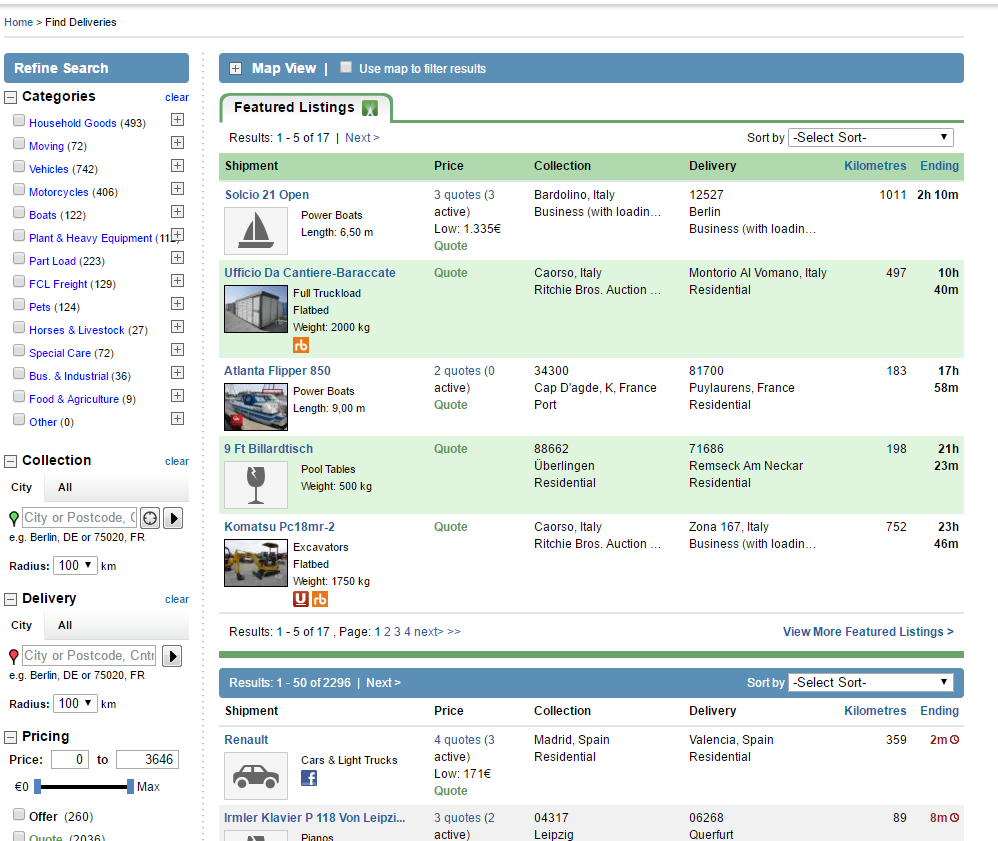
\includegraphics[width=\textwidth, scale=0.6]{img/sekcja1/uship}
\caption[uShip - widok dostępnych aukcji]{uShip - widok dostępnych aukcji\cite{uship}}
\end{figure}
Powyżej widoczny jest widok dostępnych aukcji. Wyraźnie widać podział na konkretne kategorie i możliwości wyszukiwania (lewa strona) oraz widoki poszczególnych aukcji (prawa strona).

\begin{figure}[H]
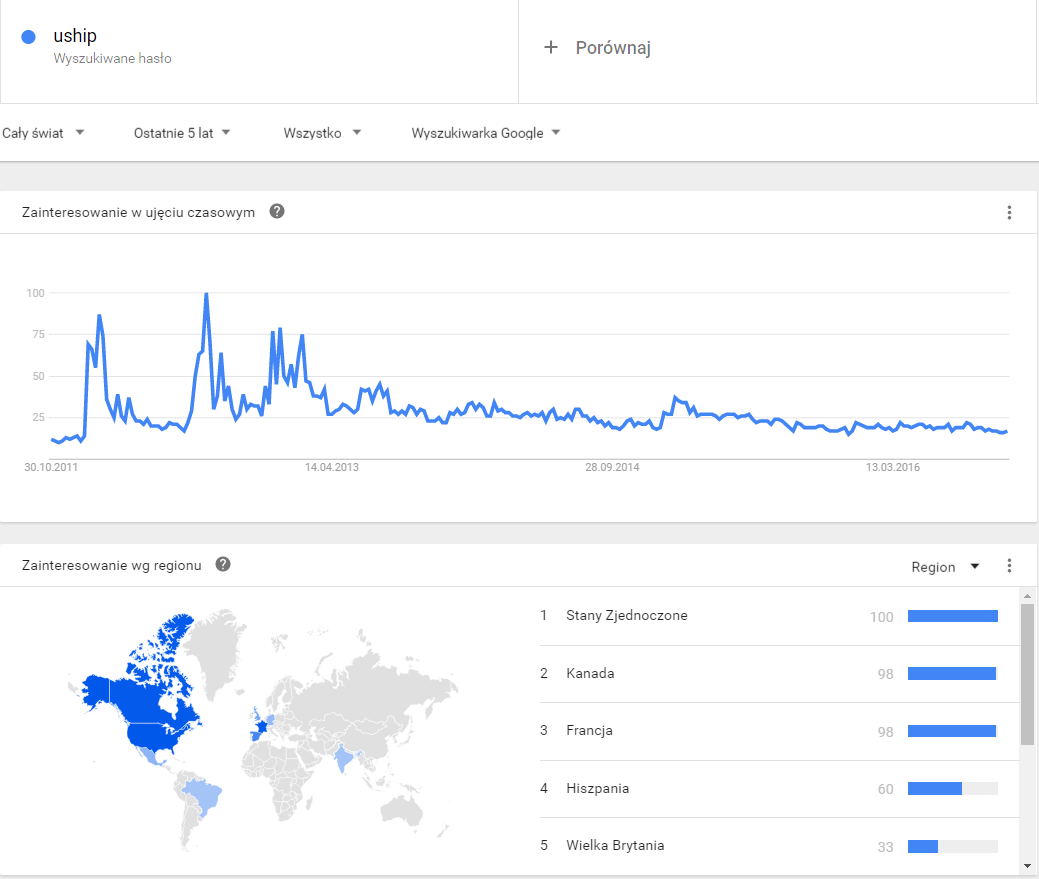
\includegraphics[width=\textwidth]{img/sekcja1/uship1}
\caption[uShip - statystyki zapytań o stronę w serwisie GoogleTrends]{uShip - statystyki zapytań o stronę w serwisie GoogleTrends\cite{googleTrends}}
\end{figure}
Powyższa grafika pokazuje statystyki częstotliwości zapytań o stronę \textit{uShip} w widocznych krajach. Wynika stąd, że
aktualne rozwiązanie jest bardzo popularne w Ameryce północnej, jednakże powoli zaczyna rozprzestrzeniać się na Europę zachodnią. W Polsce te rozwiązanie nie istnieje, dlatego też jest to dobry rynek na rozpoczęcie działalności.
\subsection{Podobne rozwiązanie - Oferteo}
Portale internetowe o podobnej tematyce na polskim rynku to jedynie \textbf{Oferteo}. 
Funkcjonalność i rozwiązanie tej aplikacji nie jest popularne w kontekście usług przewozu towarów. Strona ta realizuje niewiele założeń naszego systemu, ponieważ pozwala tylko wystawiać oferty, bez większej interakcji z potencjalnymi klientami, które są mocno ograniczone ze względu na kategorie.

\begin{figure}[H]
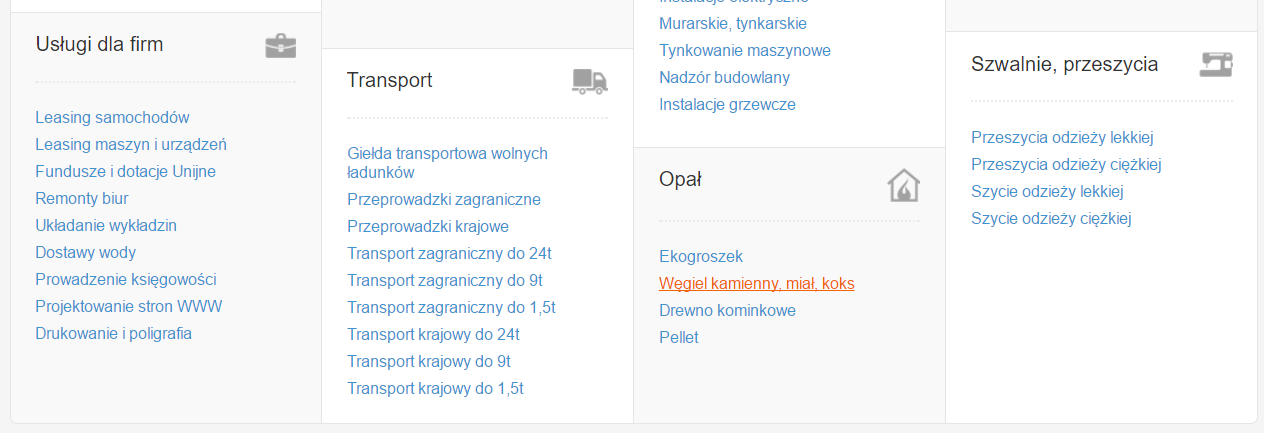
\includegraphics[width=\textwidth]{img/sekcja1/oferteoKategorie}
\caption[Oferteo - widok dostępnych kategorii]{Oferteo - widok dostępnych kategorii\cite{oferteo}}
\end{figure}
Jak widać, strona nie jest skoncentrowana na przewozach towarów lecz jest to jej jedna z funkcjonalności. Dodatkowo pokazana jest ubogą ilość kategorii.

\begin{figure}[H]
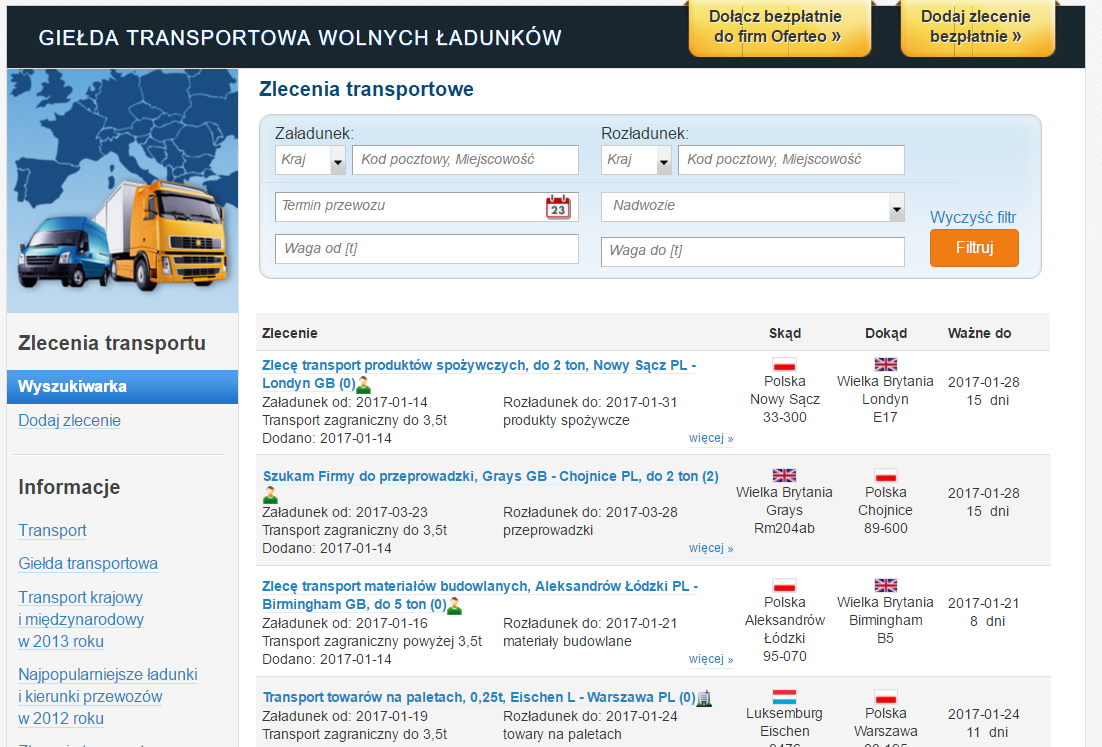
\includegraphics[width=\textwidth]{img/sekcja1/oferteoWidok}
\caption[Oferteo - widok dostępnych aukcji]{Oferteo - widok dostępnych aukcji}
\end{figure}
Oferteo nie posiada zaawansowanej wyszukiwarki aukcji. Ponadto użytkownik nie ma interakcji z ofertą, ponieważ jedynie wystawiony jest (jak już wejdzie się w konkretną aukcję) numer kontaktowy do osoby zlecającej, oraz krótki opis.

\subsection{Podobne rozwiązanie - Allegro}
Profil tej popularnej strony, wskazywałby na bardzo podobną aplikację. Jednakże główna funkcjonalność, czyli aukcje, działają na odwrotnym założeniu do wymaganego - użytkownik który da największą sumę za towar wygrywa. Nasz system wymaga, aby to najmniejsza oferta wygrała. Przez to te rozwiązanie nie nadaje się do wykorzystania. Niemniej można wzorować się na dobrze zorganizowanym systemie kategorii oraz wyszukiwania aukcji.

\subsection{Projektowana aplikacja}
Projektowana aplikacja będzie bardzo podobna do serwisu \textbf{UShip} ponieważ dzielą one wspólną idee funkcjonalności czyli aukcyjne wspomaganie przewozu towarów. Rzeczą wyróżniającą moje rozwiązanie będzie dodatkowa funkcjonalność obsługi firm które mogłyby poprzez projektowaną aplikację rozszerzyć swoją działalność.
Rozwiązanie wielojęzyczności w przypadku tej tematyki jest kluczowe ze względu na małe zapotrzebowanie na tego typu usługi w odrębnych państwach. Jak po wstępnej analizie widać w Europie nie ma jeszcze dużej konkurencji, a w Europie wschodniej jest ona zerowa.

\subsection{Podsumowanie analizy}
Aplikacje o podobnej bądź identycznej głównej funkcjonalności już istnieją, jednakże albo nie spełniają określonych wymagań, albo nie są widoczne i aktywne na polskim i wschodnio-europejskim rynku. Podsumowanie opisanych systemów najlepiej obrazuje poniższa tabela.

\begin{table}[H]
\centering
\label{my-label}
\caption{Podsumowanie analizy rynku}
\begin{tabular}{lccc}
Funkcjonalność                                                                                                                                                                   & uShip                              & Oferteo                            & \begin{tabular}[c]{@{}c@{}}Projektowany \\ system\end{tabular} \\ \hline
\multicolumn{1}{|l|}{Importowanie przedmiotów z portali aukcyjnych}                                                                                                              & \multicolumn{1}{c|}{$\harveyBallFull$}     & \multicolumn{1}{c|}{}              & \multicolumn{1}{c|}{}                                          \\ \hline
\multicolumn{1}{|l|}{Ułatwiony opis przedmiotów (kreator wystawiania przedmiotów, wiele zdjęć)}                                                                                  & \multicolumn{1}{c|}{$\harveyBallFull$}     & \multicolumn{1}{c|}{$\harveyBallQuarter$} & \multicolumn{1}{c|}{$\harveyBallFull$}                                 \\ \hline
\multicolumn{1}{|l|}{Zaznaczenie tras poprzez mapy}                                                                                                                              & \multicolumn{1}{c|}{$\harveyBallFull$}     & \multicolumn{1}{c|}{}              & \multicolumn{1}{c|}{$\harveyBallFull$}                                 \\ \hline
\multicolumn{1}{|l|}{\begin{tabular}[c]{@{}l@{}}Zaawansowany profil użytkownika \\ (zapisane metody płatności, dane, preferencje wyszukiwania)\end{tabular}}                     & \multicolumn{1}{c|}{$\harveyBallFull$}     & \multicolumn{1}{c|}{$\harveyBallQuarter$} & \multicolumn{1}{c|}{$\harveyBallFull$}                                 \\ \hline
\multicolumn{1}{|l|}{Integracja e-mail, SMS}                                                                                                                                     & \multicolumn{1}{c|}{$\harveyBallFull$}     & \multicolumn{1}{c|}{$\harveyBallFull$}     & \multicolumn{1}{c|}{$\harveyBallFull$}                                 \\ \hline
\multicolumn{1}{|l|}{\begin{tabular}[c]{@{}l@{}}Profile przewoźników mogą mieć wielu kierowców, \\ którym można zlecać zadania\end{tabular}}                                     & \multicolumn{1}{c|}{}              & \multicolumn{1}{c|}{}              & \multicolumn{1}{c|}{$\harveyBallFull$}                                 \\ \hline
\multicolumn{1}{|l|}{Wyszukiwanie/zlecanie zleceń po wielu różnych właściwościach}                                                                                               & \multicolumn{1}{c|}{$\harveyBallFull$}     & \multicolumn{1}{c|}{$\harveyBallQuarter$} & \multicolumn{1}{c|}{$\harveyBallFull$}                                 \\ \hline
\multicolumn{1}{|l|}{\begin{tabular}[c]{@{}l@{}}Wyszukiwanie zleceń wokół trasy przejazdu oraz wyznaczenie \\ nowych tras wraz z potencjalnymi nowymi zleceniami\end{tabular}}   & \multicolumn{1}{c|}{$\harveyBallHalf$} & \multicolumn{1}{c|}{}              & \multicolumn{1}{c|}{$\harveyBallFull$}                                 \\ \hline
\multicolumn{1}{|l|}{\begin{tabular}[c]{@{}l@{}}Możliwość założenia firmy(konta) przewoźniczej o większych\\ możliwościach z dostępem wielu osób w jednym momencie\end{tabular}} & \multicolumn{1}{c|}{$\harveyBallQuarter$} & \multicolumn{1}{c|}{}              & \multicolumn{1}{c|}{$\harveyBallFull$}                                 \\ \hline
\multicolumn{1}{|l|}{Integracja z aplikacją mobilną}                                                                                                                             & \multicolumn{1}{c|}{$\harveyBallFull$}     & \multicolumn{1}{c|}{}              & \multicolumn{1}{c|}{$\harveyBallHalf$}                             \\ \hline
\multicolumn{1}{|l|}{Oszacowanie kosztów i czasu przejazdu}                                                                                                                      & \multicolumn{1}{c|}{$\harveyBallHalf$} & \multicolumn{1}{c|}{}              & \multicolumn{1}{c|}{$\harveyBallFull$}                                 \\ \hline
\multicolumn{1}{|l|}{Zapisywanie trasy przejazdu, oraz pokazanie jej na mapie}                                                                                                   & \multicolumn{1}{c|}{$\harveyBallFull$}     & \multicolumn{1}{c|}{}              & \multicolumn{1}{c|}{$\harveyBallFull$}                                 \\ \hline
\multicolumn{1}{|l|}{Możliwość licytacji}                                                                                                                                        & \multicolumn{1}{c|}{$\harveyBallFull$}     & \multicolumn{1}{c|}{}              & \multicolumn{1}{c|}{$\harveyBallFull$}                                 \\ \hline
\multicolumn{1}{|l|}{Obsługa wielu języków}                                                                                                                                      & \multicolumn{1}{c|}{$\harveyBallHalf$} & \multicolumn{1}{c|}{}              & \multicolumn{1}{c|}{$\harveyBallFull$}                                                           \\ \hline
\end{tabular}
\end{table}

\paragraph{Oznaczenia}
\begin{enumerate}
\item[$\harveyBallFull$] Aplikacja posiada odpowiednią funkcjonalność w stopniu zadowalającym.
\item[$\harveyBallHalf$] Aplikacja posiada odpowiednią funkcjonalność, jednakże nie pasuje ona do profilu projektowanego systemu, bądź jest niepełna.
\item[$\harveyBallQuarter$] Aplikacja posiada słabo zaimplementowaną funkcjonalność względem wymagań projektowanego systemu.
\end{enumerate}



%%%%%%%%%%%%%%%%%%%%%%%%%%%%%%%%%%%%%%%%%%%%%%%%%%%%%%%%%%%%%%%%%%%%%%%%
%%%%%%%%%%%%%%%%%%%%%%%%%%%%%%%%%%%%%%%%%%%%%%%%%%%%%%%%%%%%%%%%%%%%%%%%
%%%%%%%%%%%%%%%%%%%%%%%%%%%%%%%%%%%%%%%%%%%%%%%%%%%%%%%%%%%%%%%%%%%%%%%%
%%%%%%%%%%%%%%%%%%%%%%%%%%%%%%%%%%%%%%%%%%%%%%%%%%%%%%%%%%%%%%%%%%%%%%%%

\newpage
\section{Omówienie koncepcji systemu}
\subsection{Ogólny opis projektu}\label{ogolny opis projektu}
Aplikacja ma za zadanie umożliwić użytkownikom wystawienia oferty wykonania usługi przewozu towaru (opisanego przez nich samych). System ma być szeroko i łatwo dostępny. Oferta po wystawieniu, ma być widoczna dla wszystkich osób, tych zalogowanych jak i niezalogowanych. Osoby które chciałby podjąć się wykonania takiej usługi muszą wygrać przetarg, który jest w postaci aukcji, działającej na zasadzie kto zaproponuje za wykonanie usługi mniej, ten wygrywa. Wystawiona usługa musi być dokładnie opisana, tak aby zleceniobiorca był w stanie bez kontaktu z zleceniodawcą, używając tylko dostępnej charakterystyki, wykonać usługę. \mbox\\
Program dodatkowo musi poza zwykłymi użytkownikami obsługiwać firmy. Firma może zarządzać przypisanymi do niej użytkownikami i rozdysponowywać wygranymi zleceniami. Konta użytkowników które podlegają firmie, działają w jej imieniu - każdy komentarz, wygrana aukcja ma być widoczne dla zarządzającego przedsiębiorstwa.

%%%%%%%%%%%%%%%%%%%%%%%%%%%%%%%%%%%%%%%%%%%%%%%%%%%%%%%%%%%%%%%%%%%%%%%%
%%%%%%%%%%%%%%%%%%%%%%%%%%%%%%%%%%%%%%%%%%%%%%%%%%%%%%%%%%%%%%%%%%%%%%%%

\subsection{Docelowi użytkownicy}
Aplikacja ma wyróżniać docelowo trzy rodzaje użytkowników:
\begin{enumerate}[1.]
\item Zwykły użytkownik - Jest dowolna osoba która może korzystać z całej podstawowej funkcjonalności aplikacji czyli wystawianie i licytacja aukcji, zarządzanie swoim kontem. Użytkownik nie może licytować własnych wystawionych aukcji. 
\item Firma - jest to specjalny użytkownik, do jego założenia wymagany jest kontakt z administratorem, bądź moderatorem aplikacji. Konto tego typu może posiadać i zarządzać wieloma kontami zwykłych użytkowników, uprzednio przypisanych do niego. W momencie przypisania, każda licytacja, wygrana bądź komentarz jest wspólny wraz z firmą zarządzającą. 
\item Moderator - jest to osoba posiadająca prawa do administrowania innymi kontami (zmiana haseł, zakończenie licytacji...) oraz jest pierwszą osobą kontaktu wszystkich rodzajów użytkowników z właścicielem aplikacji.
\end{enumerate}

\subsection{Cele funkcjonowania systemu}
Z początku głównym celem rozwoju systemu będą osoby indywidualne, jednakże z czasem ciężar ten przesuwałby się na przedsiębiorstwa.W Polsce istnieje wiele różnych firm transportowych (od typowych dużych transportów do taksówek). Skoncentrowanie się z początku na osobach indywidualnych stworzyłoby bazę użytkowników która skłoniłaby małe i średnie przedsiębiorstwa do użycia aplikacji ze względu na to, że teraz sami będą mogli wybierać towary do transportu, a użytkownicy nie muszą się martwić o szukanie odpowiedniej firmy przewozowej, gdy chodzi o nietypowy towar. 


%%%%%%%%%%%%%%%%%%%%%%%%%%%%%%%%%%%%%%%%%%%%%%%%%%%%%%%%%%%%%%%%%%%%%%%%
%%%%%%%%%%%%%%%%%%%%%%%%%%%%%%%%%%%%%%%%%%%%%%%%%%%%%%%%%%%%%%%%%%%%%%%%

\subsection{Opis funkcjonalności}
\paragraph{Jak korzystać z programu}\mbox{}\\
Użytkownik powinien bez tworzenia konta móc przejrzeć wszystkie aktualne aukcje, jednakże licytacja oraz wystawienie byłoby możliwe po uprzedniej rejestracji konta oraz zalogowaniu się. Program ma być łatwo dostępny dla użytkowników, przejrzysty i zrozumiały. Wszystkie wiadomości skierowane do użytkownika mają być maksymalnie uproszczone i jednoznaczne. Licytacja aukcji ma działać na zasadzie wypisania oferowanej kwoty oraz potwierdzenia jej, a wystawienie poprzez uzupełnienie podstawowych opisów przedmiotu oraz charakterystyki umożliwiającej jego łatwe wyszukanie.

\subsubsection{Wymagania funkcjonalne}
\begin{enumerate}[1.]
\item System musi posiadać funkcjonalność aukcyjną, gdzie jeden użytkownik wystawia aukcję, a drugi ją licytuje.
\item System musi posiadać rozbudowaną funkcjonalność wyszukiwana aukcji uwzględniającą: wyszukiwaną frazę, charakterystykę przedmiotu jak i aukcji.
%\item Wystawiona aukcja powinna posiadać dane:
%\begin{enumerate}
%\item Miejsce oraz czas odbioru i dostarczenia towaru
%\item Dowolny tytuł oraz opis słowny
%\item Historię wszystkich ofert użytkowników
%\item Opis przedmiotu, w szczególności: wymiary, waga oraz wizualna reprezentacja (zdjęcia)
%\item Charakterystyka przedmiotu, w szczególności: kategoria (np. urządzenia typu AGD, auta, ciężarówki, zwierzęta hodowlane...)
%\item Cechy szczególne przedmiotu, w szczególności: czy wymaga chłodnego środowiska, czy jest to stworzenie żyjące, czy jest to rzecz bardzo delikatna...
%\end{enumerate}
\item System ma powiadamiać użytkownika o wydarzeniach - wygrana aukcja, termin odbioru przesyłki - drogą e-mail bądź wiadomością tekstową SMS.
\item Punkt odbioru i dostarczenia towaru opisanego w aukcji, ma być widoczny na mapie z poziomu aplikacji.
\item System ma archiwizować dane, w szczególności aukcje.
\item System musi posiadać funkcjonalność obsługi firm, gdzie jedno przedsiębiorstwo posiada wielu użytkowników do zarządzania.
\item System ma posiadać możliwość wyboru języka z poziomu interfejsu użytkownika.
\item System musi posiadać narzędzia umożliwiające wysyłanie wiadomości SMS oraz e-mail.
%\item Funkcjonalność kliencka:
%\begin{enumerate}
%\item Możliwość rejestracji nowego konta
%\item Zmiana widocznego języka
%\item Administracja swoim kontem poprzez: usunięcie konta, wycofanie aukcji, zmianę danych personalnych
%\item Stworzenie aukcji
%\item Złożenie oferty aukcji
%\item Modyfikacja aukcji poprzez zmianę treści dodatkowej - widocznej w stopce 
%\item Spis aukcji - swoich jak i wygranych
%\item Opłacenie prowizji
%\end{enumerate}
%\item Funkcjonalność firmy - jest to funkcjonalność zwykłego użytkownika rozszerzona o:
%\begin{enumerate}
%\item Tworzenie nowych użytkowników przypisanych do firmy
%\item Zarządzanie kontami użytkowników poprzez zmianę ich danych, przypisanie im wygranych bądź obserwowanych aukcji
%\end{enumerate}
%\item Funkcjonalność moderatora:
%\begin{enumerate}
%\item Modyfikacje konta dowolnego użytkownika w postaci zmiany właściwości konta, zmiany danych konta, anulowanie aukcji oraz usunięcie oferty aukcji
%\item Zarządzania przychodzącymi żądaniami kontaktu ze strony użytkowników jak i przedsiębiorstw
%\item Zarządzania sporami miedzy użytkownikami
%\end{enumerate}

\end{enumerate}

\subsubsection{Wymagania niefunkcjonalne}
\begin{enumerate}[1.]
\item System ma być możliwie jak najbardziej modularny tj. funkcjonalność logiczna ma być oddzielona od wizualnej, aby łatwo można było dodać nowe interfejsy klienckie, używając zaimplementowanego już rozwiązania. Proponowanym rozwiązaniem jest implementacja aplikacji według wzorca \textit{MVC - Model View Controller}.
\item System ma być dostępny za pomocą protokołu \textit{HTTP}, oraz przez przeglądarkę internetową, dlatego też powinna być to aplikacja webowa.
\item System musi kodować hasła użytkowników, tak, aby nawet po ewentualnym wycieku danych nie były one możliwe do odczytania.
\item System ma być używalny na aktualnie trzech najpopularniejszych przeglądarkach tj. \textit{Google Chrome}, \textit{Microsoft Internet Explorer} oraz \textit{Mozilla Firefox} w wersjach nie starszych niż dwa lata od aktualnej.
\item Każdorazowe zrestartowanie systemu nie może mieć wpływu na przechowywane dane oraz istniejące aukcje.
\item Kod aplikacji powinien jasny i przejrzysty. Definicje klas i metod powinny, po przeczytaniu, sugerować swoją funkcjonalność w programie. 
\item System musi być w pełni konfigurowalny.
\item Obsługa systemu powinna być nieskomplikowana oraz intuicyjna.
\item Wszystkie wymagane funkcjonalności muszą współpracować z sobą.
\item Słowniki systemu powinny być łatwo dostępne oraz modyfikowalne.
\item Użytkownik wystawiający aukcje powinien posiadać podstawowe narzędzia edycji tekstu (zmiana czcionki, kolor tekstu, listowanie...) przy tworzeniu opisu aukcji.
\item System należy zaimplementować używając możliwie tylko darmowych rozwiązań, preferowanymi narzędziami są:
\begin{enumerate}
\item Baza danych: \textit{Microsoft SQL Server}, \textit{MariaDB}, \textit{MySQL}, \textit{PostgreSQL}.
\item System logiczny: \textit{Java}, \textit{C\#}, \textit{C++} z uwzględnieniem \textit{frameworków}, odpowiednio \textit{Spring} bądź \textit{.NET}
\item Aplikacja kliencka: \textit{AngularJS}, \textit{Angular2}, \textit{PHP}
\end{enumerate} 
\item System musi być odporny na ataki typu \textit{SQL injection}.
\item System musi posiadać edytowalną możliwość ustawienia długości sesji poszczególnych użytkowników.
\item System powinien posiadać narzędzia monitorujące podstawowe czynności takie jak ilość zapytań na daną jednostkę czasu, ilość użytkownika czy historię akcji użytkownika.
\item Użytkownik powinien otrzymać oszacowane koszty przewozu towaru.
\end{enumerate}

%%%%%%%%%%%%%%%%%%%%%%%%%%%%%%%%%%%%%%%%%%%%%%%%%%%%%%%%%%%%%%%%%%%%%%%%
%%%%%%%%%%%%%%%%%%%%%%%%%%%%%%%%%%%%%%%%%%%%%%%%%%%%%%%%%%%%%%%%%%%%%%%%
%%%%%%%%%%%%%%%%%%%%%%%%%%%%%%%%%%%%%%%%%%%%%%%%%%%%%%%%%%%%%%%%%%%%%%%%
%%%%%%%%%%%%%%%%%%%%%%%%%%%%%%%%%%%%%%%%%%%%%%%%%%%%%%%%%%%%%%%%%%%%%%%%
\newpage
\section{Analiza dostępnych narzędzi}
Ze względu na upodobania i umiejętności, narzędzia programistyczne użyte do tworzenia serwera zostały zwężone do technologii związanych z Javą.
\subsection{Baza danych}

Pod uwagę zostały wzięte dwie technologie - \textit{Microsoft SQL Server} oraz \textit{MySQL} z uwagi na doświadczenie. \mbox\\
Pierwsza z nich, technologia \textit{Microsoftu} jest renomowaną i bardzo dobrze znaną bazą danych, jednakże faworyzowanymi przez nią narzędziami są pochodzące od tej samej firmy rozwiązania. Ograniczeniem tej bazy są środowiska na których można ją łatwo zainstalować oraz obsłużyć z których wykluczony jest system \textit{Linux}. \mbox\\

Następną technologią jest \textit{MySQL}. Popularna i dobrze znana każdemu baza danych. Jest łatwa w obsłudze oraz można ją zainstalować na każdym środowisku. Darmowa wersja zapewnia wszystkie niezbędne narzędzia, począwszy od partycji kończąc na statystykach.\mbox\\
Finalnie jako technologia bazodanowa została wybrana baza \textit{MySQL}, głównie ze względów na łatwą możliwość instalacji na większości używanych systemach.

\subsection{Serwer}
Serwer logiczny aplikacji będzie wykonany w technologii \textit{Java} przy użyciu rekomendowanego \textit{frameworku - Spring} ze względu na moje umiejętności. Jednakże system ma być wielomodułowy, dlatego też należy wybrać technologię , którą serwer będzie udostępniać informacje. Pod uwagę zostały wzięte dwie możliwości. Pierwszą z nich jest udostępnianie wiadomości za pomocą wbudowanych narzędzi \textit{Spring - RESTful API} poprzez przekazywanie danych używając struktury typu \textit{JSON - JavaScript Object Notation}. Drugim rozwiązaniem jest użycie także zaimplementowanego protokołu w \textit{Spring'u} - \textit{SOAP}. \mbox\\

Rozwiązania te różnią się głównie sposobem prezentacji danych. Pierwsze z nich wystawia dane, używając łatwego do przetworzenia obiektu poprzez języki używane przy tworzeniu stron internetowych. Drugie rozwiązanie oferuje pokazanie informacji poprzez język znaczników - \textit{XML}.\mbox\\
Ze względu, iż architektura \textit{SOAP} jest już dość stara i nowsze technologie mogą jej nie uwzględniać w swojej implementacji, zdecydowałem się na nowszy i łatwo czytelny sposób wystawiania informacji poprzez technologię \textit{RESTful API}.
\subsection{Aplikacja kliencka}
W wymaganiach aplikacji zostały uwzględnione trzy technologie \textit{AngularJS}, \textit{Angular2} oraz \textit{PHP}.
\paragraph{PHP}\mbox\\ 

Stare, jednakże ciągle rozwijane rozwiązanie. Ma one swoje problemy, głównie związane ze skalowalnością. Jednakże każdy większy problem ma swoje znane rozwiązanie bądź sposób ominięcia go, ale zazwyczaj są to bardzo skomplikowane procedury. Ze względu na możliwą wielkość aplikacji oraz ważny jej aspekt - skalowalność, język ten nie zostanie użyty.
\paragraph{AngularJS}\mbox\\

Język stworzony przez korporacje \textit{Google}. Jest to bardzo dobra technologia do tworzenia dużych aplikacji internetowych. Szczególnie jest ona używana poprzez większe firmy które tworzą projekty wymagające dużego nakładu czasu oraz czytelnej struktury. Cechuje on się, w odróżnieniu do innych technologii \textit{webowych}, obiektową hierarchią poszczególnych modułów aplikacji, oraz kontrolą typów poprzez wprowadzenie języka \textit{TypeScript} (który kompiluje kod źródłowy do języka \textit{JavaScript}). Istnieje bardzo dużo udostępnionych rozwiązań poprzez innych użytkowników którzy także aktywnie pomagają w rozwiązywaniu problemów.
\paragraph{Angular2}\mbox\\

Jest to kontynuacja technologii \textit{AngularJS}, jednakże ilość zmian jest znacząca na tyle, że nie da się przeprojektować aplikacji napisanej w \textit{AngularJS} do \textit{Angular2}. Wprowadzono w niech dużo nowości oraz ulepszono nowe rozwiązania. Całe skupienie firmy \textit{Google} jest skoncentrowane właśnie na tej technologii. Jest ona relatywnie młoda, finalna wersja została wprowadzona dopiero na przełomie października i listopada, jednakże istnieje już spora grupa aktywnych użytkowników którzy rozwijają tę technologię poprzez udostępnianie swoich rozwiązań.\mbox\\
Ze względu na to, iż projektowana aplikacja będzie dużym systemem zdecydowałem się na rozwiązanie firmy \textit{Google}. Jednakże problemem było zdecydowanie się czy użyć nowszych czy starszych technologii. Za \textit{AngularJS} stał jej wiek i stabilność, a za \textit{Angular2} łatwiejsze i nowocześniejsze rozwiązania kosztem mniejszej stabilności.\mbox\\
Finalnie wybrana została technologia \textit{Angular2} ze względu, iż w tej technologii \textit{Google} pokłada największe nadzieje oraz pieniądze na rozwój, czego naturalnym efektem jest stopniowe porzucanie \textit{AngularJS}.

%%%%%%%%%%%%%%%%%%%%%%%%%%%%%%%%%%%%%%%%%%%%%%%%%%%%%%%%%%%%%%%%%%%%%%%%
%%%%%%%%%%%%%%%%%%%%%%%%%%%%%%%%%%%%%%%%%%%%%%%%%%%%%%%%%%%%%%%%%%%%%%%%

\subsection{Podsumowanie wyboru technologii}

Wszystkie technologie są darmowe oraz bogato opisane przykładami na swoich stronach internetowych, które zostały załączone na poniższej liście. Każda z technologii posiada na stronie domowej własną dokumentacje jak i można znaleźć dużo przykładów i opisów tworzonych przez samych, niezależnych, internautów. Dodatkowo wymienione, nieopisane wyżej narzędzia są standardowymi wyborami przy pracy z odpowiadającymi im \textit{frameworkami} np. \textit{Java - Spring + Hibernate}, dowolna technologia aplikacji klienckiej dostępnej poprzez przeglądarkę internetową - \textit{Bootstrap}. 
\paragraph{Wybrane technologie}
\begin{enumerate}[1.]
\item Baza danych - \textit{MySQL}\cite{mysql}
\item Back-end - \textit{Java 8}\cite{java8} wraz ze wsparciem \textit{frameworków} - \textit{Spring (RESTful Services, Security OAuth2, Springboot)}\cite{spring}, \textit{Hibernate}\cite{hibernate}, oraz system zarządzania i budowy projektu \textit{Apache Maven}\cite{maven}
\item Front-end -\textit{Angular2}\cite{angular2} pod wsparciem ulepszonego JavaScript - \textit{TypeScript} - specjalnie pod tę technologie. Dodatkowo do upiększania strony \textit{Bootstrap 3}\cite{bootstrap}.
\end{enumerate}
Implementacja projektu będzie tworzona przy pomocy środowiska programistycznego \textit{IntelliJ IDE}\cite{intelliJ} na licencji studenckiej. Projekt będzie zapisywany na darmowym repozytorium \textit{BitBucket}\cite{bitbucket} umożliwiającym łatwą kontrolę wersji. Obydwa wybory są subiektywne, nie wpływają na realizację jak i utrzymanie projektu.
%%%%%%%%%%%%%%%%%%%%%%%%%%%%%%%%%%%%%%%%%%%%%%%%%%%%%%%%%%%%%%%%%%%%%%%%
%%%%%%%%%%%%%%%%%%%%%%%%%%%%%%%%%%%%%%%%%%%%%%%%%%%%%%%%%%%%%%%%%%%%%%%%
%%%%%%%%%%%%%%%%%%%%%%%%%%%%%%%%%%%%%%%%%%%%%%%%%%%%%%%%%%%%%%%%%%%%%%%%
%%%%%%%%%%%%%%%%%%%%%%%%%%%%%%%%%%%%%%%%%%%%%%%%%%%%%%%%%%%%%%%%%%%%%%%%
\newpage
\section{Projekt systemu}

\subsection{Architektura systemu}
System będzie działać w oparciu o model \textit{MVC - Model View Controller}\cite{mvc}.
Architektura ta wyróżnia następujące główne węzły aplikacji:
\begin{enumerate}
\item[Model:] Baza danych w technologii \textit{MySQL} przechowywująca dane.
\item[Kontroler:] Serwer napisany w technologii \textit{Java} w oparciu o \textit{frameworki} \textit{Spring} oraz \textit{Hibernate}, który ma za zadanie przetwarzać wszystkie informacje.
\item[Widok:] Podstawowym widokiem dla zwykłego użytkownika będą aplikacje klienckie napisane w technologii \textit{Angular2} oraz na urządzenia mobilne \textit{Android}. Jednakże te aplikacje będą korzystały i odpowiednio przystosowywały dane dla klienta które będą wystawiane na widoku podstawowym czyli \textit{RESTful API} - interfejsie aplikacji do którego można będzie zwrócić się odpowiednimi zapytaniami \textit{HTTP, np. GET, POST...}, aby pobrać bądź zmodyfikować dane znajdujące się w bazie danych.
\end{enumerate}

Powyższe rozwiązanie graficznie przedstawia poniższy rysunek:
\begin{figure}[H]
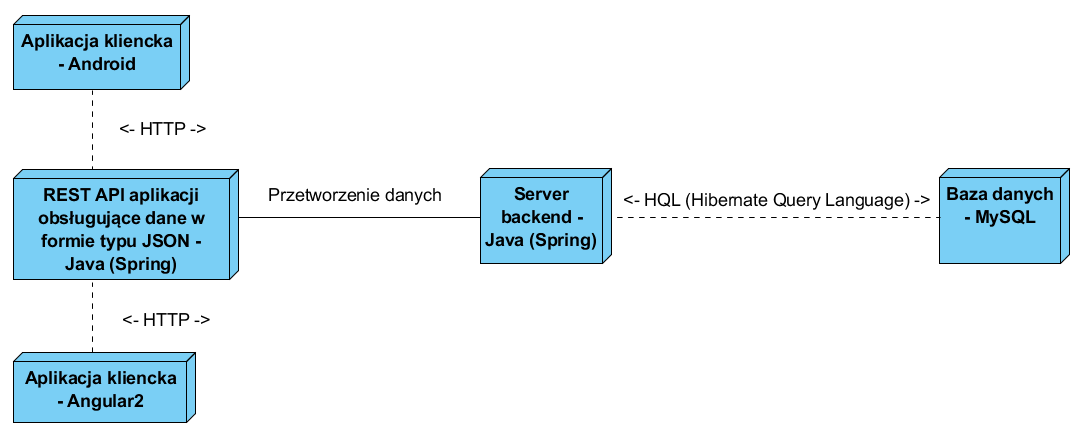
\includegraphics[width=\textwidth]{img/sekcja2/architekturaAplikacji}
\caption[Architektura systemu]{Architektura systemu}
\end{figure}

\paragraph{Optymalizacja i skalowalność aplikacji}\mbox{}\\
Aplikacja ma za zadanie przetworzyć wiele względnie prostych zapytań w krótkiej jednostce czasu, dlatego też system należy przygotować na taką okoliczność. Poniżej znajduję się lista kluczowych dla aplikacji rozwiązań które umożliwią płynną pracę aplikacji przy dużym obciążeniu:
\begin{enumerate}
\item Baza danych jak i \textit{serwer backendowy} powinny zostać uruchomione jak najbliżej siebie np. w jednej podsieci, albo najlepiej na jednej maszynie, ponieważ od reakcji między aplikacją serwerową, a bazą zależy czas odpowiedzi na zapytanie przychodzące z zewnątrz. Typowego przetwarzania danych nie jest dużo, więc można ten aspekt pominąć.
\item Niektóre zapytania będą częściej wykorzystywane niż inne dlatego należy stale monitorować obciążenie poszczególnych rodzajów zapytań jak i \textit{endpointów} aplikacji, aby doraźnie optymalizować bazę danych jak i same zapytania. Proponowanym rozwiązaniem dla takiego problemu jest przeniesienie bazy danych na technologie \textit{Oracle}. Bazy danych w tej technologii słyną z bardzo dobrej optymalizacji zapytań. Ostatecznym rozwiązaniem byłoby rozdzielenie bazy danych na klika węzłów, jednakże wtedy skomplikowałaby się struktura samych zapytań, a na dodatek należałoby zmienić charakterystykę samej bazy na nierelacyjną (takie rozwiązanie stworzyłby podwaliny pod system rozproszony).
\end{enumerate}

%%%%%%%%%%%%%%%%%%%%%%%%%%%%%%%%%%%%%%%%%%%%%%%%%%%%%%%%%%%%%%%%%%%%%%%%
%%%%%%%%%%%%%%%%%%%%%%%%%%%%%%%%%%%%%%%%%%%%%%%%%%%%%%%%%%%%%%%%%%%%%%%%

\subsection{Diagramy klas}
Diagram klas ściśle łączy się z diagramem związków encji, dlatego też szczegółowy opis widocznych rysunków znajduję się w sekcji \hyperref[Diagramy związków encji]{diagramy związków encji}.
\begin{figure}[H]
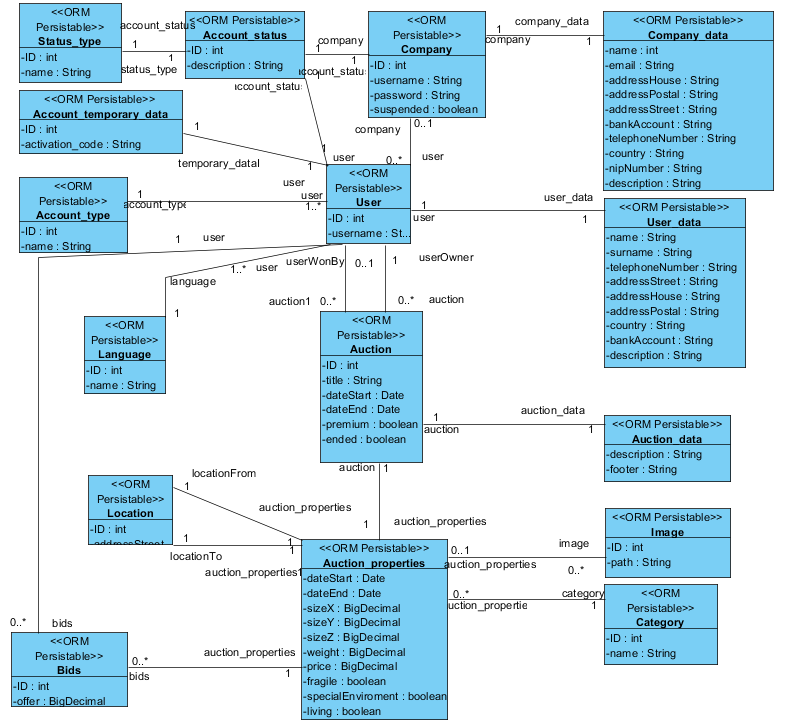
\includegraphics[width=\textwidth]{img/sekcja2/diagramKlas}
\caption[Diagram klas]{Diagram klas}
\end{figure}

%%%%%%%%%%%%%%%%%%%%%%%%%%%%%%%%%%%%%%%%%%%%%%%%%%%%%%%%%%%%%%%%%%%%%%%%
%%%%%%%%%%%%%%%%%%%%%%%%%%%%%%%%%%%%%%%%%%%%%%%%%%%%%%%%%%%%%%%%%%%%%%%%
\newpage
\subsection{Diagramy związków encji} \label{Diagramy związków encji}
\begin{figure}[H]
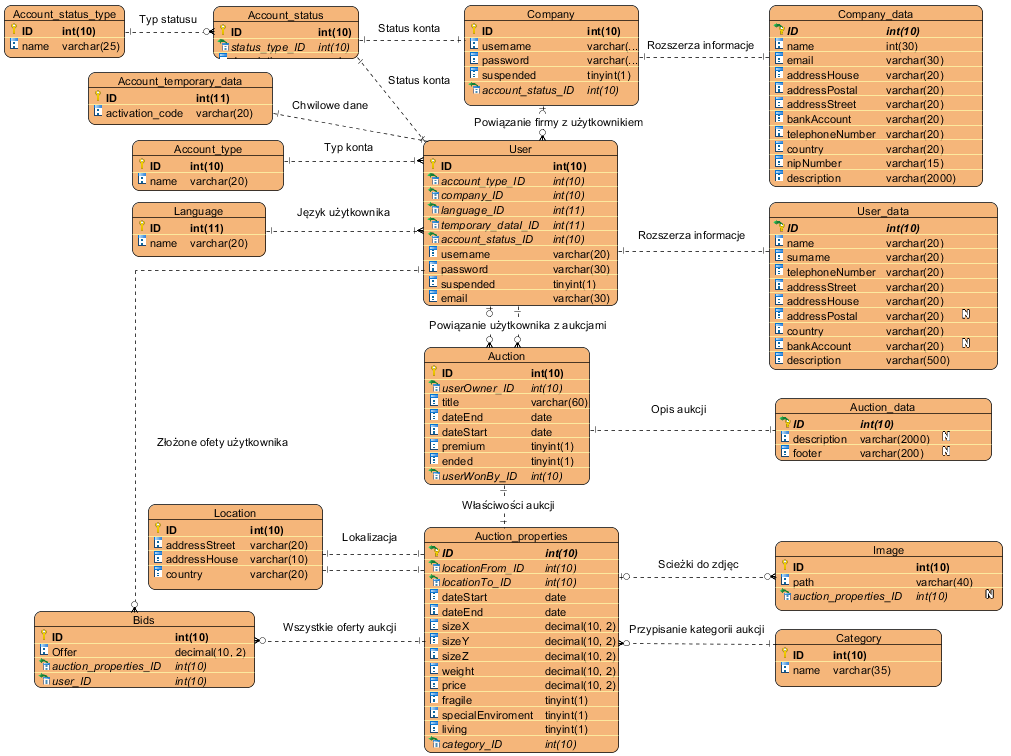
\includegraphics[width=\textwidth]{img/sekcja2/bazaDanych}
\caption[Diagram związków encji]{Diagram związków encji}
\end{figure}
\mbox{}\\
Powyższy diagram związków encji należy rozumieć następująco: \\
Firma (wraz ze swoimi danymi) może posiadać wielu użytkowników. Każdy użytkownik posiada swoje konto (wraz z danymi), któremu można przypisać język oraz specyficzny typ konta jak np. premium, albo zablokowane. Każde konto może mieć wiele aukcji swoich, jak i wiele aukcji które licytuje. Sama aukcja ma swoje specyficzne właściwości jak i sam opis oraz historię wszystkich zalicytowanych sum pieniędzy.
\mbox{}\\
Diagram ten pokazuje główną część bazy danych, dodatkowo istnieje kilka encji związanych między innymi z autoryzacją (tokeny), wspomaganiem \textit{frameworku} \textit{Hibernate}.
%%%%%%%%%%%%%%%%%%%%%%%%%%%%%%%%%%%%%%%%%%%%%%%%%%%%%%%%%%%%%%%%%%%%%%%%
%%%%%%%%%%%%%%%%%%%%%%%%%%%%%%%%%%%%%%%%%%%%%%%%%%%%%%%%%%%%%%%%%%%%%%%%
\newpage
\subsection{Diagramy przypadków użycia}

\begin{figure}[H]
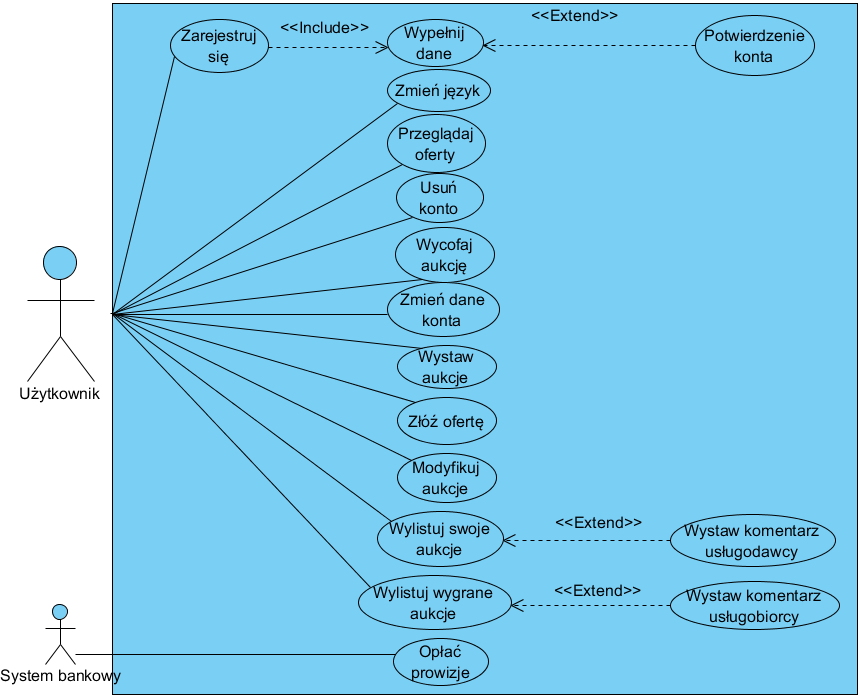
\includegraphics[width=\textwidth]{img/sekcja2/uzytkownikPU}
\caption[Diagram przypadków użycia - użytkownik aplikacji]{Diagram przypadków użycia - użytkownik aplikacji}
\end{figure}

\paragraph{Szczegółowe definicje przypadków użycia dla diagramu użytkownika}\mbox{}\\
\begin{enumerate}[1.]
\item Zarejestruj się
\begin{enumerate}
\item[Cel użycia:] Rejestracja nowego konta do użytkowania aplikacji
\item[Warunek początkowy:] Brak
\item Wejście na stronę rejestracji.
\item Wypełnienie wymaganych danych i potwierdzenie akcji - nazwa użytkownika, hasło, poczta e-mail, imię, nazwisko, numer telefonu, dane adresowe.
\item Przesłanie danych do \textit{serweru backendowego} poprzez odpowiednie żądanie \textit{HTTP}.
\item Walidacja danych.
\item zapisanie danych do bazy danych poprzez \textit{serwer backendowy}.
\item Wysłanie maila z kodem aktywującym konto do użytkownika w celu weryfikacji konta e-mail.
\item (Opcjonalne) Wpisanie kodu aktywacyjnego i porównanie go z kodem, który został wysłany, w przypadku pozytywnym aktywacja konta, negatywnym – możliwość wysłania maila z kodem ponownie.
\end{enumerate}

\item Zmień język
\begin{enumerate}
\item[Cel użycia:] Zmiana wyświetlanego języka
\item[Warunek początkowy:] Brak
\item Wybranie wyświetlanego języka z możliwych, widoczne informację są zapisane po stronie klienta, więc nie ma potrzeby odwoływania się do bazy danych.
\end{enumerate}

\item Przeglądaj oferty
\begin{enumerate}
\item[Cel użycia:] Wyszukanie aukcji przy użyciu dostępnych narzędzi 
\item[Warunek początkowy:] Brak
\item Wybierz kategorie – zaznaczenie kategorii, z których aukcje mają zostać wyświetlone.
\item Wpisz frazę do wyszukiwarki – wpisanie słów kluczowych, po których zostaną wyszukane aukcje.
\item Przesłanie danych do \textit{serweru backendowego} poprzez odpowiednie żądanie \textit{HTTP}.
\item Odczytanie danych z bazy i wysłanie ich do klienta.
\end{enumerate}

\item Usuń konto
\begin{enumerate}
\item[Cel użycia:] Usunięcie konta
\item[Warunek początkowy:] Zalogowanie się na istniejące konto
\item Ponowne zalogowanie się do konta w celach weryfikacji - otrzymanie dodatkowego tokena umożliwiającego wykonywanie dodatkowych operacji przez krótki okres czasu.
\item Potwierdzenie usunięcia konta.
\end{enumerate}

\item Wycofaj aukcje
\begin{enumerate}
\item[Cel użycia:] Anulowanie istniejącej aukcji
\item[Warunek początkowy:] Zalogowanie się na istniejące konto
\item Wybranie aukcji do anulowania
\item Ponowne zalogowanie się do konta w celach weryfikacji - otrzymanie dodatkowego tokena umożliwiającego wykonywanie dodatkowych operacji przez krótki okres czasu.
\item Potwierdzenie anulowania aukcji.
\end{enumerate}

\item Zmień dane konta
\begin{enumerate}
\item[Cel użycia:] Zmiana danych konta użytkownika
\item[Warunek początkowy:] Zalogowanie się na istniejące konto
\item Edycja dostępnych danych.
\item Ponowne zalogowanie się do konta w celach weryfikacji - otrzymanie dodatkowego tokena umożliwiającego wykonywanie dodatkowych operacji przez krótki okres czasu.
\item Potwierdzenie zmiany danych.
\end{enumerate}

\item Wystaw aukcję
\begin{enumerate}
\item[Cel użycia:] Wystawienie aukcji przez użytkownika
\item[Warunek początkowy:] Zalogowanie się na istniejące konto
\item Pobranie wymaganych danych do wystawienia aukcji .
\item Walidacja danych w kontekście poprawności oraz bezpieczeństwa.
\item Potwierdzenie wystawienia aukcji wraz z ekranem podglądu.
\end{enumerate}

\item Złóż ofertę
\begin{enumerate}
\item[Cel użycia:] Złożenie oferty licytacyjnej
\item[Warunek początkowy:] Zalogowanie się na istniejące konto oraz wejście na stronę konkretnej aukcji
\item Wypełnienie pola z informacją o składanej ofercie pieniężnej.
\item Walidacja danych w kontekście poprawności (kwota musi być mniejsza od ostatniej najmniejszej oferty) oraz bezpieczeństwa.
\item Potwierdzenie.
\end{enumerate}

\item Modyfikuj aukcję
\begin{enumerate}
\item[Cel użycia:] Modyfikacja istniejącej i aktywnej aukcji
\item[Warunek początkowy:] Zalogowanie się na istniejące konto
\item Wybranie aukcji z pośród własnych wystawionych, aktualnych aukcji.
\item Możliwość edycji danych aktualnej aukcji jedynie w zakresie dodanej stopki, inne dane nie mogą zostać zmienione.
\item Zapis do bazy – zapisanie zmian do bazy danych.
\end{enumerate}

\item Wylistuj swoje/wygrane aukcje
\begin{enumerate}
\item[Cel użycia:] Wyświetlenie wszystkich własnych/wygranych aukcji
\item[Warunek początkowy:] Zalogowanie się na istniejące konto 
\item Wejście na odpowiednią zakładkę.
\item Wyszukanie aukcji poprzez dostępne narzędzia.
\end{enumerate}

\item Wystaw komentarz usługodawcy
\begin{enumerate}
\item[Cel użycia:] Wystawienie komentarza usługodawcy
\item[Warunek początkowy:] Zalogowanie się na istniejące konto oraz wybranie zakończonej aukcji w celu skomentowania
\item Skomentowanie realizacji zlecenia poprzez użytkownika.
\item Potwierdzenie.
\end{enumerate}

\item Wystaw komentarz usługobiorcy
\begin{enumerate}
\item[Cel użycia:] Zalogowanie się na istniejące konto oraz wybranie zakończonej aukcji w celu skomentowania
\item[Warunek początkowy:] Zalogowanie się na istniejące konto.
\item Skomentowanie realizacji zlecenia poprzez usługodawce.
\item Potwierdzenie.
\end{enumerate}

\item Opłać prowizję
\begin{enumerate}
\item[Cel użycia:] Opłacenie prowizji za korzystanie z usług aplikacji
\item[Warunek początkowy:] Zalogowanie się na istniejące konto
\item Wyświetlenie wszystkich niezapłaconych prowizji oraz ich podsumowanie.
\item Przekieruj na stronę banku – przekierowanie płatności do zewnętrznych aplikacji bankowych oferujących taką funkcjonalność.
\item Otrzymanie potwierdzenia zapłaty z aplikacji obsługującej płatności.
\end{enumerate}


\end{enumerate}

\begin{figure}[H]
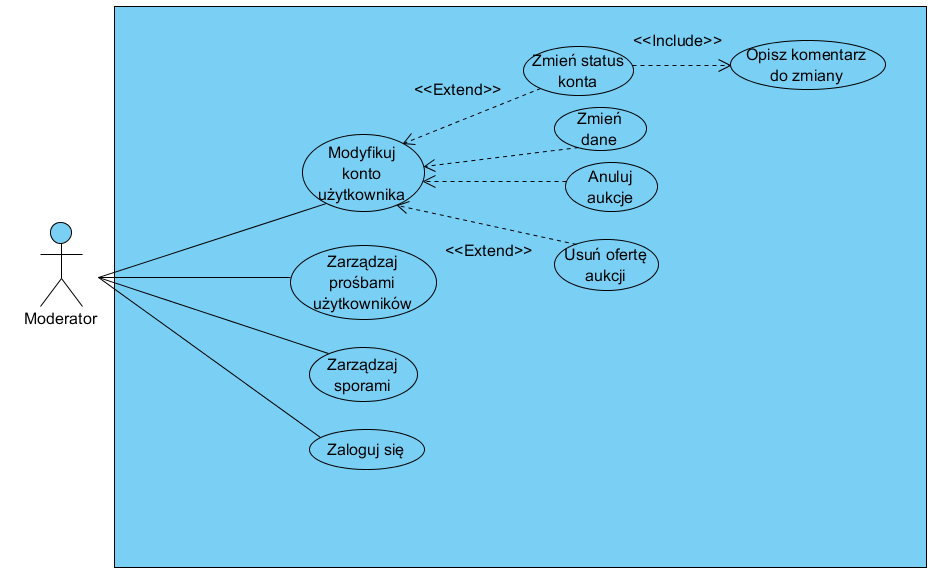
\includegraphics[width=\textwidth]{img/sekcja2/moderatorPU}
\caption[Diagram przypadków użycia - moderator aplikacji]{Diagram przypadków użycia - moderator aplikacji}
\end{figure}

\paragraph{Szczegółowe definicje przypadków użycia dla diagramu moderatora}\mbox{}\\
\begin{enumerate}[1.]

\item Zmień status konta
\begin{enumerate}
\item[Cel użycia:] Usunięcie konta
\item[Warunek początkowy:] Zalogowanie się na istniejące konto oraz wybranie zakładki Modyfikuj konto użytkownika
\item Zmiana status konta użytkownika (np. z aktywnego na zablokowany).
\item Opisanie komentarza przyczyny zmiany statusu konta.
\end{enumerate}

\item Zmień dane
\begin{enumerate}
\item[Cel użycia:] Zmiana danych konta użytkownika
\item[Warunek początkowy:] Zalogowanie się na istniejące konto oraz wybranie zakładki Modyfikuj konto użytkownika
\item Zmiana danych konta użytkownika (np. hasła bądź adresu e-mail).
\end{enumerate}

\item Anuluj aukcje
\begin{enumerate}
\item[Cel użycia:] Anulowanie aktywnej aukcji
\item[Warunek początkowy:] Zalogowanie się na istniejące konto oraz wybranie zakładki Modyfikuj konto użytkownika
\item Zakończenie wybranej, aktywnej aukcji.
\end{enumerate}

\item Zarządzaj prośbami użytkowników
\begin{enumerate}
\item[Cel użycia:] Zarządzanie prośbami użytkowników
\item[Warunek początkowy:] Zalogowanie się na istniejące konto
\item Wejście na odpowiednią zakładkę.
\item Przeczytanie kolejnej wolnej prośby oraz próba rozwiązania jej.
\item Przesłanie odpowiedzi ze statusem rozwiązania do użytkownika.
\item Zamknięcie prośby.
\end{enumerate}

\item Zarządzaj sporami
\begin{enumerate}
\item[Cel użycia:] Zarządzanie sporami użytkowników
\item[Warunek początkowy:] Zalogowanie się na istniejące konto
\item Wejście na odpowiednią zakładkę.
\item Przeczytanie kolejnej wolnej prośby oraz próba rozwiązania jej.
\item Przesłanie odpowiedzi ze statusem rozwiązania do użytkownika.
\item Zamknięcie prośby.
\end{enumerate}

\end{enumerate}
%%%%%%%%%%%%%%%%%%%%%%%%%%%%%%%%%%%%%%%%%%%%%%%%%%%%%%%%%%%%%%%%%%%%%%%%
%%%%%%%%%%%%%%%%%%%%%%%%%%%%%%%%%%%%%%%%%%%%%%%%%%%%%%%%%%%%%%%%%%%%%%%%
\newpage
\subsection{Diagramy aktywności}
Są to tylko przykładowe przypadki, ponieważ każda akcja użytkownika jest trywialna i nie wymaga żadnych skomplikowanych działań (kilka kliknięć myszki oraz wypełnienie widocznego pola). Ze względu na ich trywialność i powtarzalność, nie ma sensu tworzyć logicznie takich samych kolejnych diagramów aktywności.

\begin{figure}[H]
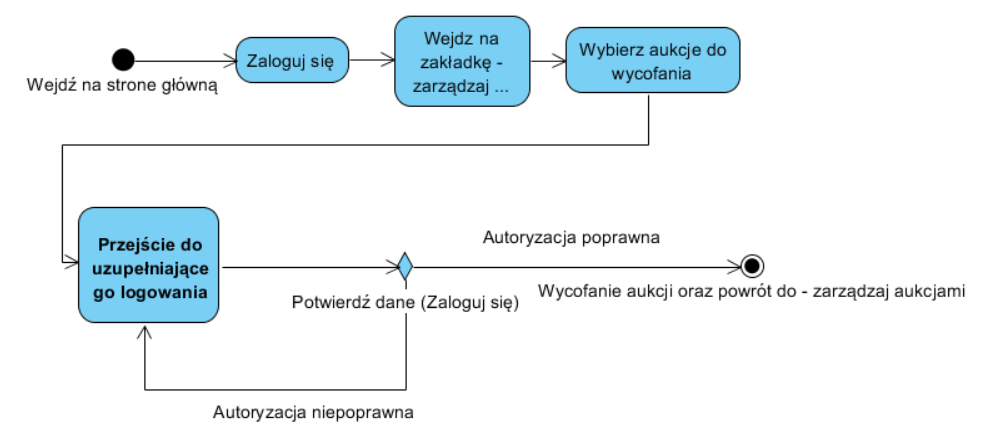
\includegraphics[width=\textwidth]{img/sekcja2/wycofajAukcjeAD}
\caption[Diagram aktywności - wycofanie aukcji]{Diagram aktywności - wycofanie aukcji}
\end{figure}

\begin{figure}[H]
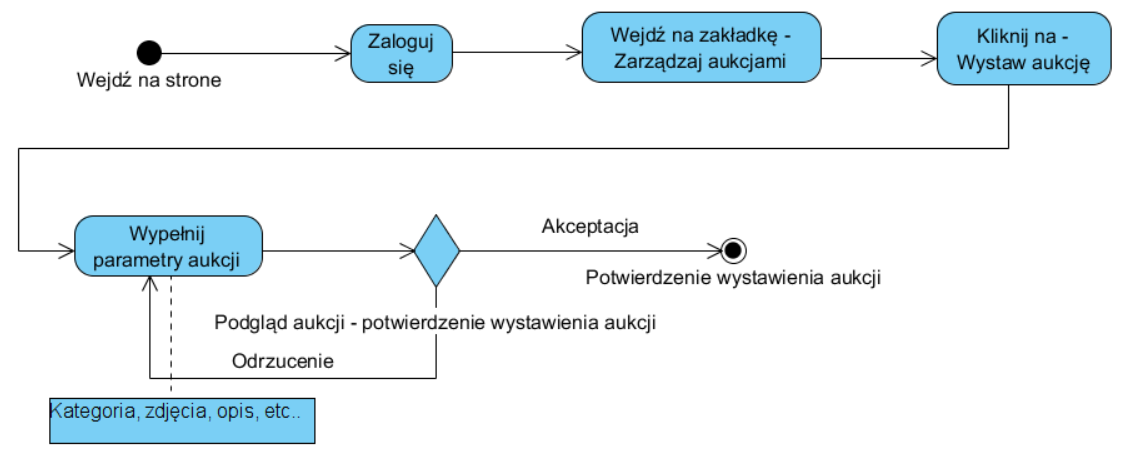
\includegraphics[width=\textwidth]{img/sekcja2/wystawAukcjeAD}
\caption[Diagram aktywności - wystawienie aukcji]{Diagram aktywności - wystawienie aukcji}
\end{figure}

\begin{figure}[H]
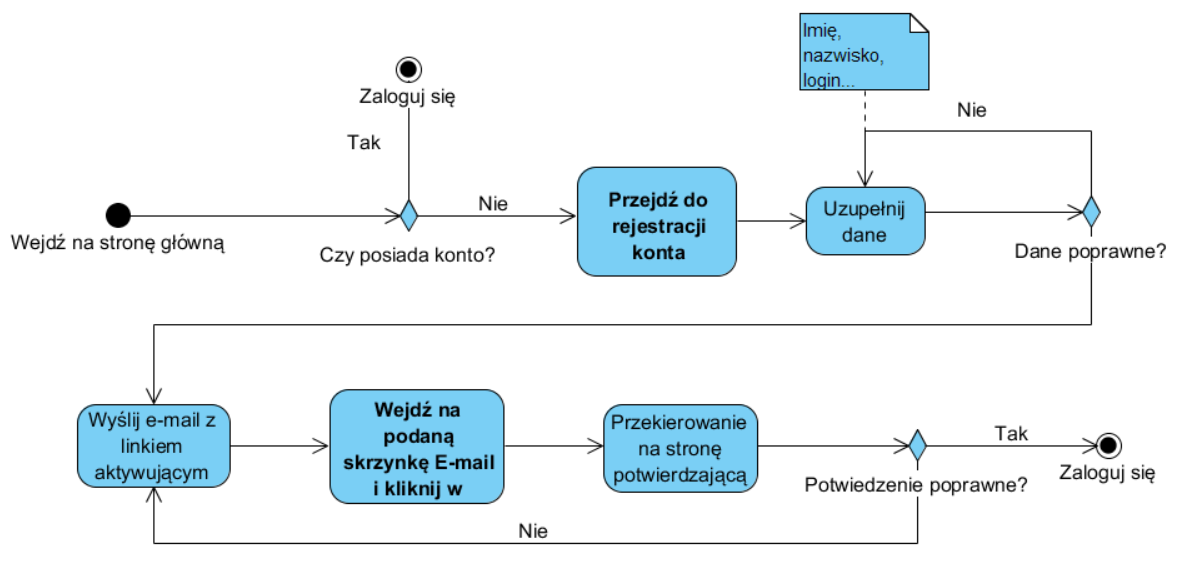
\includegraphics[width=\textwidth]{img/sekcja2/rejestracjaKontaAD}
\caption[Diagram aktywności - rejestracja konta]{Diagram aktywności - rejestracja konta}
\end{figure}
%%%%%%%%%%%%%%%%%%%%%%%%%%%%%%%%%%%%%%%%%%%%%%%%%%%%%%%%%%%%%%%%%%%%%%%%
%%%%%%%%%%%%%%%%%%%%%%%%%%%%%%%%%%%%%%%%%%%%%%%%%%%%%%%%%%%%%%%%%%%%%%%%
\newpage
\subsection{Diagramy sekwencji}
Poniższe diagramy pokazują wszystkie moduły działania aplikacji poprzez cały swój zakres. Każda sekwencja w tej aplikacji jest bardzo podobna do siebie ponieważ wszystkie akcje działają w oparciu o model MVC (Model-View-Controller) co oznacza, że każde pytanie ze strony użytkownika, które wymaga jakichkolwiek danych musi przejść przez \textit{serwer backendowy}, który przechowuje całą logikę aplikacji oraz walidacje. Aplikacja kliencka posiada walidacje takie, aby ułatwić klientowi przejście przez walidacje serwerowe, logiki decyzyjnej nie posiada.

\begin{figure}[H]
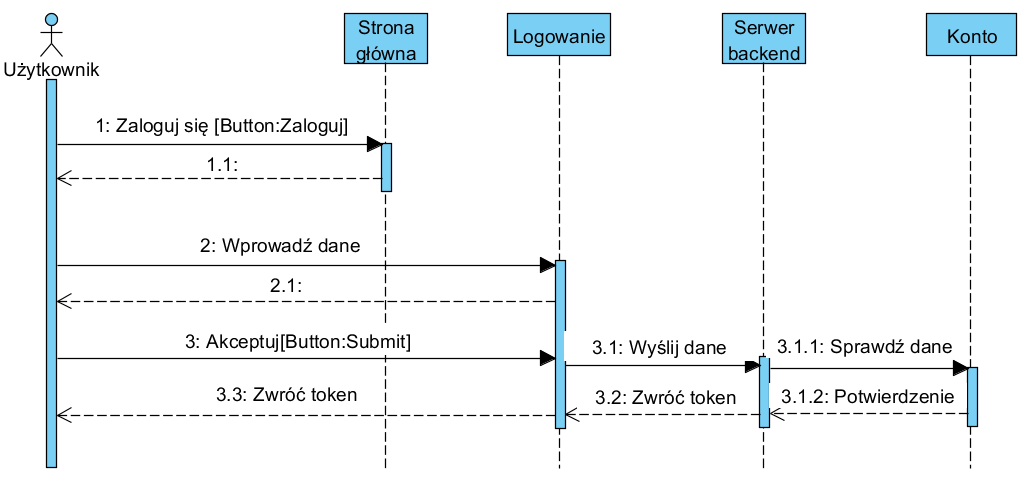
\includegraphics[width=\textwidth]{img/sekcja2/logowanieSD}
\caption[Diagram sekwencji - logowanie]{Diagram sekwencji - logowanie}
\end{figure}
Powyższy diagram pokazuje sekwencje logowania klienta do aplikacji.
\paragraph{Oznaczenia tzw. \textit{linii życia}}
\begin{enumerate}[1.]
\item Strona główna - jest to \textit{endpoint} strony głównej/reprezentacyjnej która ukazuje się użytkownikowi po wejściu na stronę
\item Logowanie - jest to \textit{endpoint} logowania do aplikacji
\item Serwer backend - jest to serwer aplikacji napisany w języku \textit{Java} który posiada całą logikę decyzyjną jak i wystawione \textit{RESTful API}
\item Konto - oznacza konto klienckie w rozumieniu danych przechowywanych w bazie danych
\end{enumerate}

\begin{figure}[H]
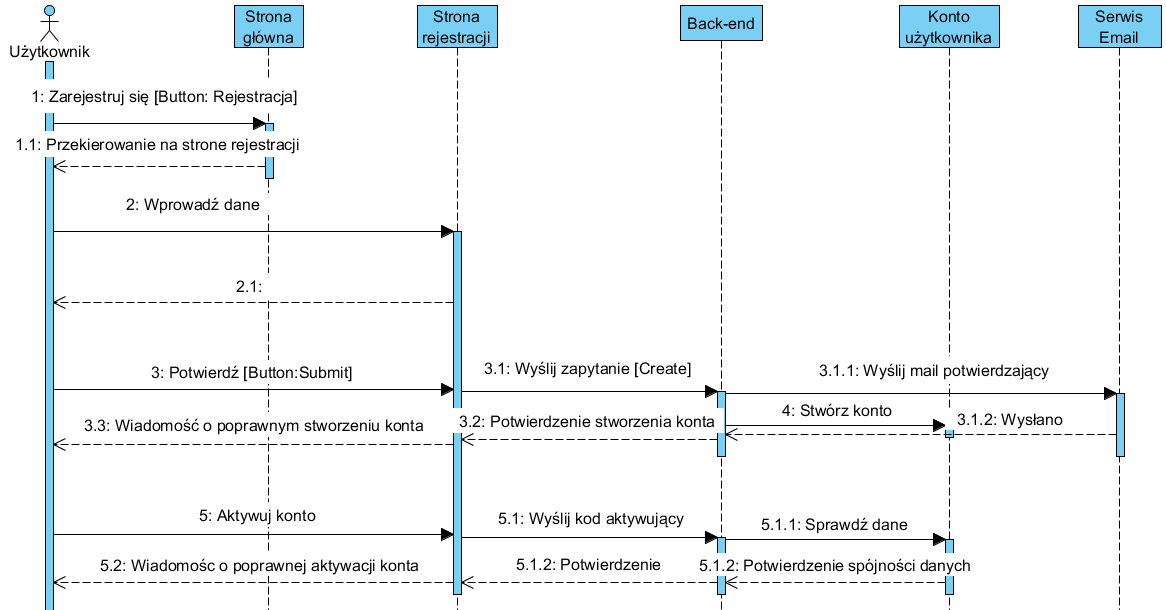
\includegraphics[width=\textwidth]{img/sekcja2/rejestracjaSD}
\caption[Diagram sekwencji - rejestracja użytkownika]{Diagram sekwencji - rejestracja użytkownika}
\end{figure}
Powyższy diagram pokazuje sekwencje rejestracji nowego użytkownika aplikacji.
\paragraph{Oznaczenia tzw. \textit{linii życia}}
\begin{enumerate}[1.]
\item Strona główna - jest to \textit{endpoint} strony głównej/reprezentacyjnej która ukazuje się użytkownikowi po wejściu na stronę
\item Strona rejestracji - jest to \textit{endpoint} rejestracji nowego konta
\item Back-end - jest to serwer aplikacji napisany w języku \textit{Java} który posiada całą logikę decyzyjną jak i wystawione \textit{RESTful API}
\item Konto użytkownika- oznacza konto klienckie w rozumieniu danych przechowywanych w bazie danych
\item Serwis Email - jest to usługa za pośrednictwem której można wysłać pocztę elektroniczną na wskazany adres
\end{enumerate}


\begin{figure}[H]
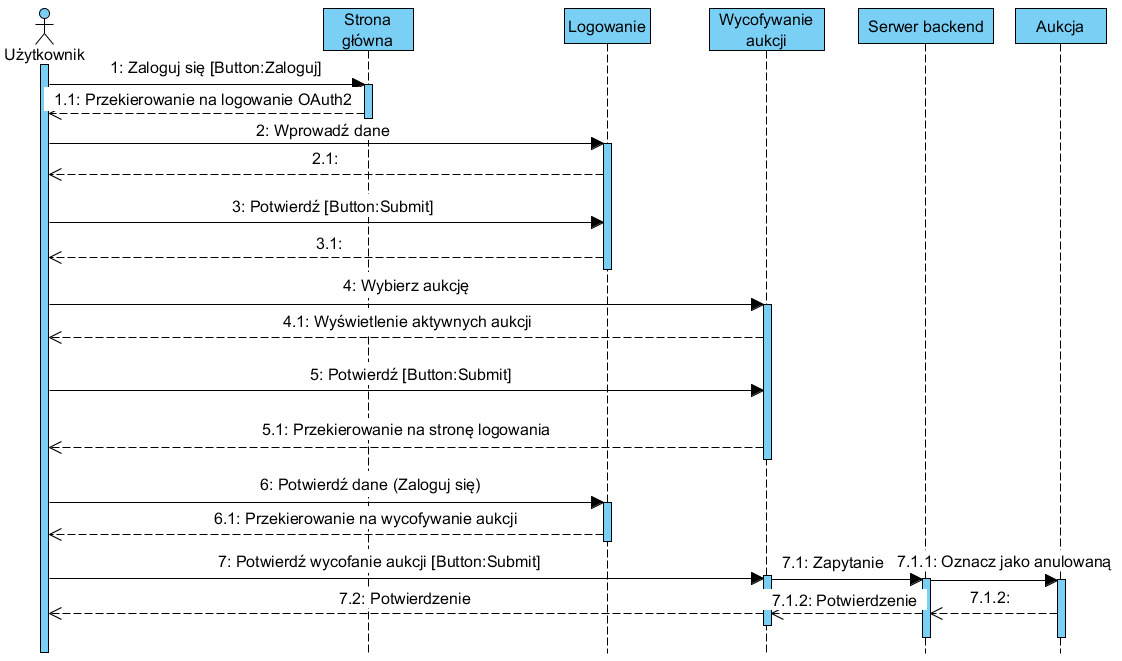
\includegraphics[width=\textwidth]{img/sekcja2/wycofajAukcjeSD}
\caption[Diagram sekwencji - anulowanie aukcji]{Diagram sekwencji - anulowanie aukcji}
\end{figure}
\paragraph{Oznaczenia tzw. \textit{linii życia}}
Powyższy diagram pokazuje sekwencje anulowania aukcji klienta.
\begin{enumerate}[1.]
\item Strona główna - jest to \textit{endpoint} strony głównej/reprezentacyjnej która ukazuje się użytkownikowi po wejściu na stronę
\item Logowanie - jest to \textit{endpoint} logowania do aplikacji
\item Wycofywanie aukcji - jest to strona na której użytkownik może wybrać aukcje do anulowania
\item Serwer backend - jest to serwer aplikacji napisany w języku \textit{Java} który posiada całą logikę decyzyjną jak i wystawione \textit{RESTful API}
\item Aukcja - jest to reprezentacja aukcji danego użytkownika
\end{enumerate}

%%%%%%%%%%%%%%%%%%%%%%%%%%%%%%%%%%%%%%%%%%%%%%%%%%%%%%%%%%%%%%%%%%%%%%%%
%%%%%%%%%%%%%%%%%%%%%%%%%%%%%%%%%%%%%%%%%%%%%%%%%%%%%%%%%%%%%%%%%%%%%%%%

\subsection{Opis mechanizmów bezpieczeństwa}
\paragraph{Mechanizmy zabezpieczające hasła}\mbox{}\\
Docelowo wersja produkcyjna aplikacji posiadać kodowane hasła systemem SHA512. Hash ten ma za zadanie ukryć hasła użytkowników przed ewentualnym wyciekiem bazy danych.
Dodatkowo wersja produkcyjna oprogramowania ukrywa wszelkie błędy komunikacji z baza danych w celu uniknięcia pokazania informacji poufnych.

\paragraph{Mechanizmy autoryzacyjne}\mbox{}\\
Do autoryzacji użytkowników mają być używane tokeny, które będą czasowym identyfikatorem użytkownika. Użytkownik będzie musiał zalogować się raz na określony czas (dane logowania będą przesyłane z użyciem protokołu SSL) co zmniejsza ryzyko kradzieży danych. Aby dostać się do ważniejszych funkcji systemu, posiadacz tokena o podstawowych uprawnieniach będzie musiał zalogować się ponownie z użyciem tokena, hasła i loginu.

\paragraph{Mechanizmy przetwarzające zapytania po stronie serwera}\mbox{}\\
Do walidacji zapytań zostaną użyte systemy wychwytujące niedozwolone znaki (np. znaki ucieczki, kod \textit{XML}), lub też kawałki kodu napisanego w \textit{HTML, JavaScript, Java}. Przykładową biblioteką oferującą takie rozwiązanie jest \href{https://www.owasp.org/index.php/Category:OWASP_AntiSamy_Project#tab=Main}{OWASP AntiSamy Project}\cite{owaspAntiSammyProject}.

%%%%%%%%%%%%%%%%%%%%%%%%%%%%%%%%%%%%%%%%%%%%%%%%%%%%%%%%%%%%%%%%%%%%%%%%
%%%%%%%%%%%%%%%%%%%%%%%%%%%%%%%%%%%%%%%%%%%%%%%%%%%%%%%%%%%%%%%%%%%%%%%%

\newpage
\subsection{Opis \textit{endpointów}}
\subsubsection{\textit{Backend}}
Opisane poniżej \textit{endpointy}, są to adresy \textit{RESTful API} na które można wysłać odpowiednie żądania \textit{HTTP}, aby otrzymać odpowiedź.
Wszystkie parametry są przekazywane jako typ tekstowy \textit{String}. Na \textit{serwerze backendowym} zostają one parsowane.
Struktura linku jest następująca:\\*www.domena.com/\{nazwa endpointa\}?argument1=\ldots\&argument2=\ldots\\*gdzie:
\begin{enumerate}[1.]
\item \{nazwa endpointa\} - \textit{opcje}
\\*Opis słowny funkcjonalności endpointa
\begin{enumerate}[a.]
\item argument1 - opis słowny
\item argument2 - \ldots
\item \ldots
\end{enumerate}
\item \ldots
\end{enumerate}

Opcje:\\*Token - możliwość wykonania operacji tylko za pomocą tokena dostarczanego poprzez serwis logujący, umożliwiający uwierzytelnienie użytkownika. Token ten powinien zostać przekazany poprzez nagłówek żadania \textit{HTTP}.

\paragraph{\textit{Endpointy}}
\begin{enumerate}[1.]

\item createUser
\\*Zapisanie nowego użytkownika do bazy
\begin{enumerate}[a.]
\item username – nazwa użytkownika
\item password – hasło użytkownika
\end{enumerate}

\item activateUser
\\*Aktywacja nowego użytkownika za pomocą przysłanego linka na adres e-mail
\begin{enumerate}[a.]
\item activationID – unikatowy kod aktywacyjny wygenerowany dla konta
\item userID – unikatowy identyfikator użytkownika na bazie
\end{enumerate}

\item listMyAuctions - Token
\\*Spis aukcji użytkownika
\begin{enumerate}[a.]
\item categories – lista kategorii
\item userID – identyfikator uzytkownika
\end{enumerate}

\item listWonAuctions - Token
\\*Spis aukcji które użytkownik wygrał
\begin{enumerate}[a.]
\item categories – lista kategorii
\item userID – identyfikator uzytkownika
\end{enumerate}

\item listActiveAuctions - Token
\\*Spis aukcji które są aktywne i były licytowane przez użytkownika chociaż raz
\begin{enumerate}[a.]
\item categories – lista kategorii
\item userID – identyfikator uzytkownika
\end{enumerate}

\item listAuctions
\\* Spis aukcji względem kategorii i wyszukanej frazy
\begin{enumerate}[a.]
\item searchPhrase – słowa kluczowe, dla których mają zostać wyszukane rekordy
\item categories – lista kategorii
\item parameters – lista dodatkowych parametrów
\end{enumerate}

\item showAuction\/\{auctionID\}
\\*Wyświetlenie pojedyńczej aukcji
\begin{enumerate}[a.]
\item \{auctionID\} – identyfikator aukcji
\end{enumerate}

\item login 
\\*Logowanie użytkownika
\begin{enumerate}[a.]
\item username – nazwa użytkownika
\item password – hasło użytkownika
\end{enumerate}

\item bidAuction/\$\{auctionID\} - Token
\\*Złożenie oferty dla konkretnej aukcji
\begin{enumerate}[a.]
\item userID – identyfikator użytkownika
\item offer – oferta
\item \$\{auctionID\} – identyfikator aukcji
\end{enumerate}

\item createAuction - Token
\begin{enumerate}[a.]
\item userID – identyfikator Użytkownika
\item parametry – tj. lokacja, daty etc.
\end{enumerate}

\item securedModifyUser - Token
\\*Modyfikuj dane użytkownika - zabezpieczone dodatkowym tokenem
\begin{enumerate}[a.]
\item userID – identyfikator użytkownika
\item username – nazwa użytkownika
\item password – hasło użytkownika
\item e-mail – poczta użytkownika
\end{enumerate}

\item securedDeleteAuction - Token
\\*Wycofaj aukcję - zabezpieczone dodatkowym tokenem
\begin{enumerate}[a.]
\item userID – identyfikator użytkownika
\item auctionID – identyfikator aukcji
\end{enumerate}

\end{enumerate}
\subsubsection{\textit{Frontend}}
Aplikacja kliencka nie będzie zawierać wielu adresów, ponieważ służy ona do pomocy w obsłudze danych. Jeden \textit{endpoint} może posiadać funkcjonalność obsługi wielu \textit{endpointów serweru backendowego}. Dokładny opis tych punktów znajduję się w dziale
\hyperref[Szkice i funkcjonalność aplikacji klienckiej]{szkice i funkcjonalność aplikacji klienckiej}.
\begin{figure}[H]
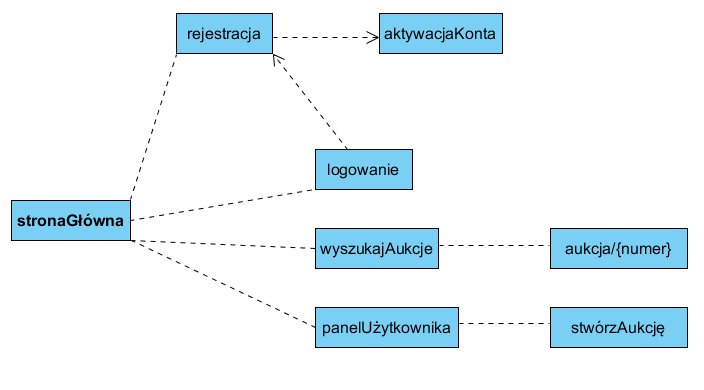
\includegraphics[width=\textwidth]{img/sekcja2/mapaEndpointowFrontend}
\caption[Mapa \textit{endpointów} aplikacji klienckiej]{Mapa \textit{endpointów} aplikacji klienckiej}
\end{figure}
\paragraph{Objaśnienia}\mbox{}\\
\begin{enumerate}[1.]
\item Linia przerywana, bez strzałek: oznacza, iż istnieją odnośniki przekierowujące pomiędzy dwoma połączonymi daną linią adresami.
\item Linia przerywana, ze strzałką: oznacza, iż na konkretny adres strony, z danego punktu, można dostać się tylko jednostronnie (\textit{np. z logowania można przejść do rejestracji, natomiast z rejestracji do logowania już nie}).
\end{enumerate}


%%%%%%%%%%%%%%%%%%%%%%%%%%%%%%%%%%%%%%%%%%%%%%%%%%%%%%%%%%%%%%%%%%%%%%%%
%%%%%%%%%%%%%%%%%%%%%%%%%%%%%%%%%%%%%%%%%%%%%%%%%%%%%%%%%%%%%%%%%%%%%%%%
\newpage
\subsection{Szkice i funkcjonalność aplikacji klienckiej}\label{Szkice i funkcjonalność aplikacji klienckiej}
Poniżej znajdują się wszystkie opisane \textit{endpointy} stron dostępnych z poziomu aplikacji klienckiej. Jedyny adres który nie został uwzględniony czyli \textit{stronaGłówna}, nie jest tutaj uwzględniony ponieważ ta strona ma zawierać tylko bieżące informacje więc jej wygląd będzie dopasowywany na bieżąco w zależności od wymagań klienta.

\subsubsection{Logowanie}
\begin{figure}[H]
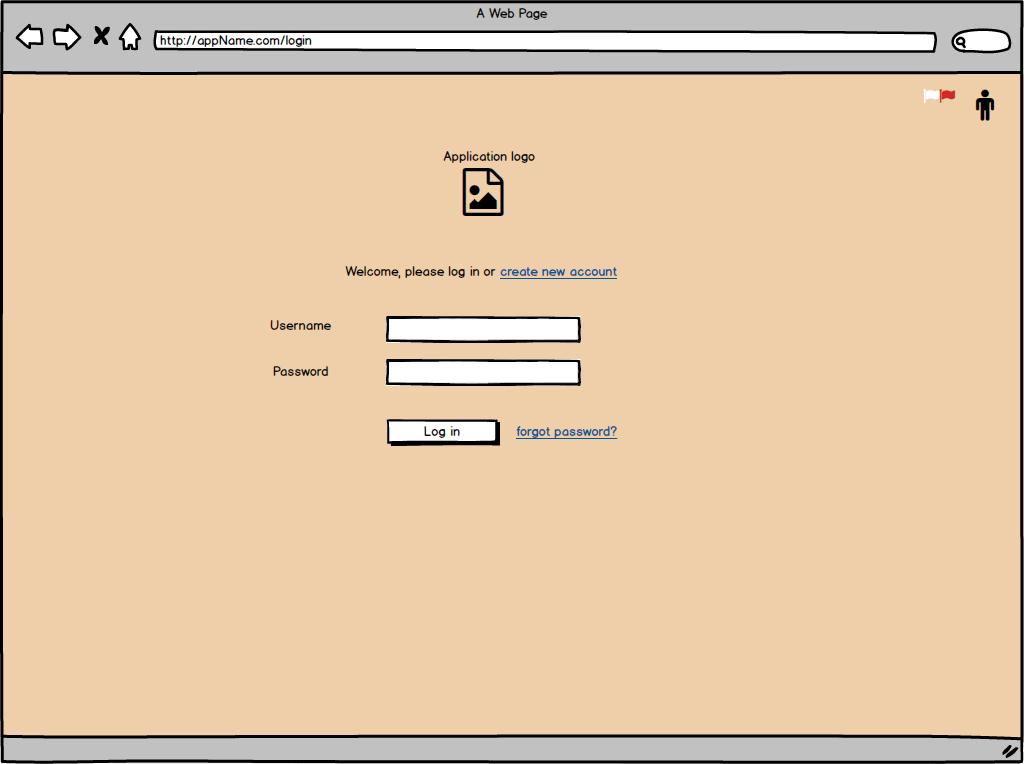
\includegraphics[width=\textwidth]{img/sekcja2/loginScreenMock}
\caption[Szkice aplikacji - logowanie użytkownika]{Szkice aplikacji - logowanie użytkownika}
\end{figure}

\paragraph{Funkcjonalność}\mbox{}\\
Strona ta służy jako interfejs logowania. Użytkownik ma za zadanie podać dane logowania. Następnie aplikacja wysyła zapytanie z danymi do \textit{serwera backendowego}. W odpowiedzi pozytywnej otrzymuje token, a negatywnej nic. Token ma być przechowywany lokalnie, przy użyciu technologii \textit{Local Storage} - nowocześniejszej wersji \textit{Cookie, tzw. ciasteczek}.
\paragraph{Walidacja}\mbox{}\\
\begin{enumerate}[1.]
\item Pole tekstowe z nazwą użytkownika lub adresem e-mail: brak
\item Pole tekstowe z hasłem: brak
\end{enumerate}

%%%%%%%%%%%%%%%%%%%%%%%%%%%%%%%%%%%%%%%%%%%%%%%%%%%%%%%%%%%%%%%%%%%%%%%%
%%%%%%%%%%%%%%%%%%%%%%%%%%%%%%%%%%%%%%%%%%%%%%%%%%%%%%%%%%%%%%%%%%%%%%%%

\subsubsection{Wyszukiwanie aukcji}
\begin{figure}[H]
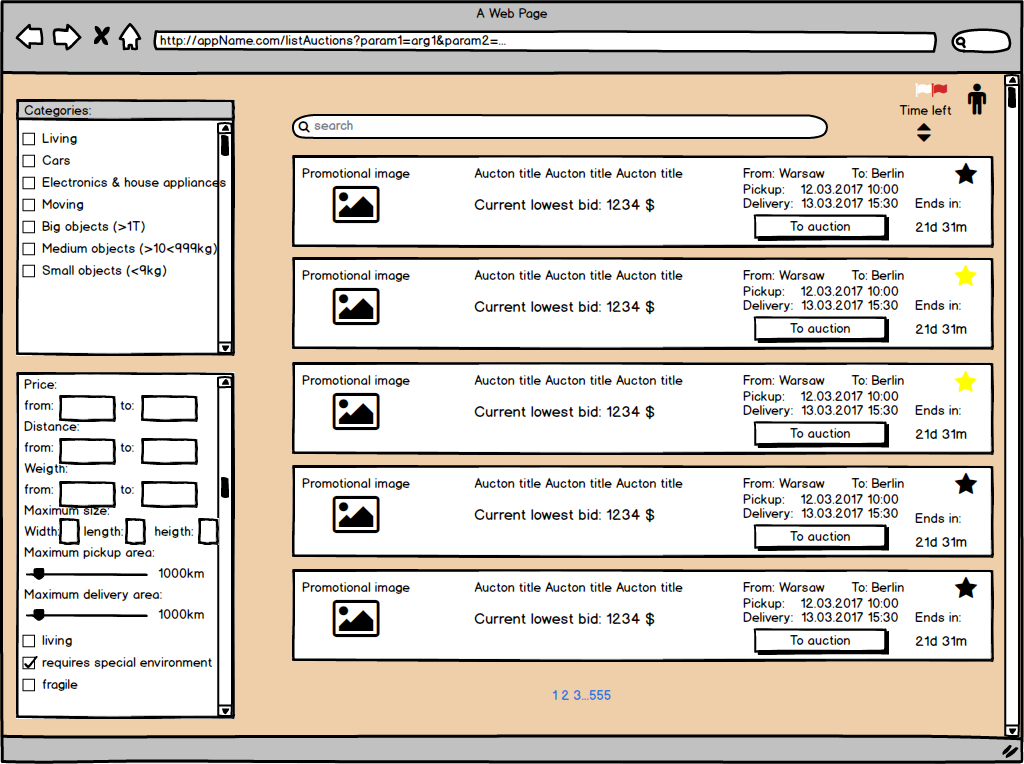
\includegraphics[width=\textwidth]{img/sekcja2/auctionSearchMock}
\caption[Szkice aplikacji - wyszukiwanie aukcji]{Szkice aplikacji - wyszukiwanie aukcji}
\end{figure}

\paragraph{Funkcjonalność}\mbox{}\\
Strona ta zapewnia funkcjonalność zaawansowanego wyszukiwania aukcji z uwzględnieniem wielu parametrów, pochodzących z różnych elementów: okienka wyszukiwania, okienka zaznaczenia kategorii specyficznych dla towarów (cena, waga itp.). Domyślnie wyświetlane będą aukcje w kolejności od najmniejszego pozostałego czasu do zakończenia. Po zaznaczeniu odpowiednich kategorii i wysłania zapytania, strona powinna otrzymać listę aukcji odpowiadającą zapytaniu. Lista ta powinna zostać wyświetlona w widoczny sposób (prostokąty pod elementem wyszukiwania stron). Te elementy powinny posiadać przycisk po którym użytkownik może przejść do interesującej go aukcji.
\paragraph{Walidacja}\mbox{}\\
\begin{enumerate}[1.]
\item Pole tekstowe wyszukiwania danych: walidacja typu SQL i Java.
\item Pola tekstowe z zaawansowanym wyszukiwaniem (cena, dystans...): brak
\end{enumerate}
%%%%%%%%%%%%%%%%%%%%%%%%%%%%%%%%%%%%%%%%%%%%%%%%%%%%%%%%%%%%%%%%%%%%%%%%
%%%%%%%%%%%%%%%%%%%%%%%%%%%%%%%%%%%%%%%%%%%%%%%%%%%%%%%%%%%%%%%%%%%%%%%%

\subsubsection{Rejestracja nowego użytkownika}
\begin{figure}[H]
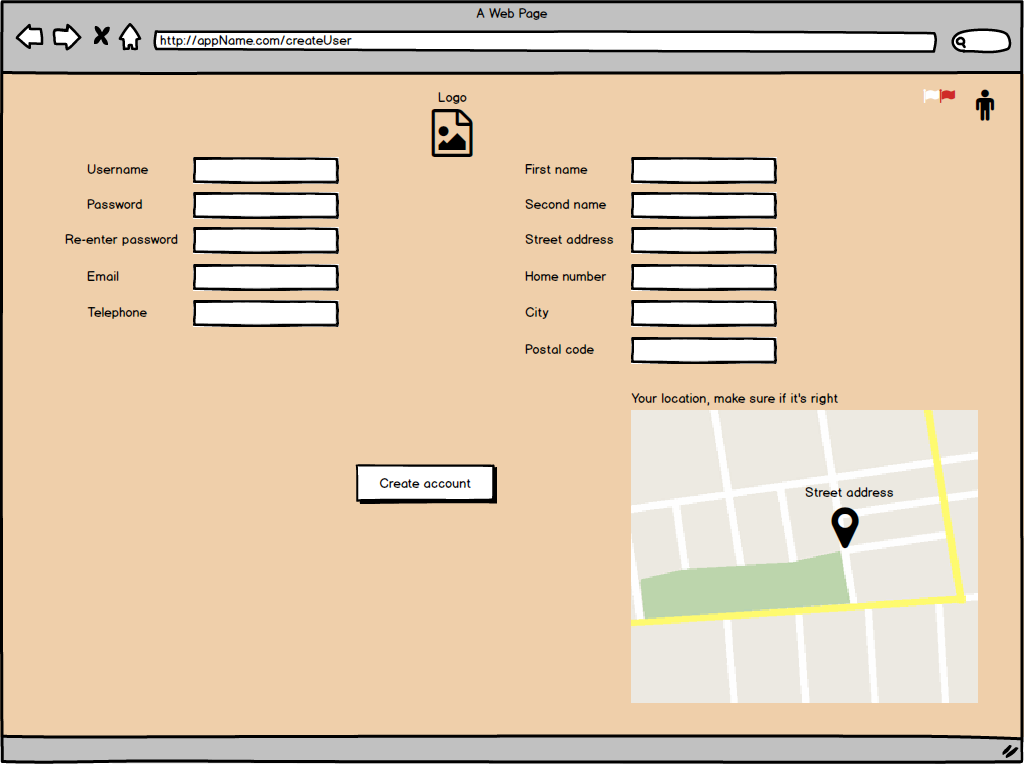
\includegraphics[width=\textwidth]{img/sekcja2/createUserMock}
\caption[Szkice aplikacji - rejestracja nowego użytkownika]{Szkice aplikacji - rejestracja nowego użytkownika}
\end{figure}

\paragraph{Funkcjonalność}\mbox{}\\
Strona umożliwia zarejestrowanie konta nowego użytkownika w systemie. Aplikacja kliencka wysyła dane do serwera, a w odpowiedzi otrzymuje czy konto zostało założone poprawnie czy nie. Dodatkowo wyświetlana jest mapa która pokazuje zapisany adres. Użytkownika nie ma z niej innej interakcji niż poprzez uzupełnienie pól tekstowych.
\paragraph{Walidacja}\mbox{}\\
\begin{enumerate}[1.]
\item Pole tekstowe nazwy użytkownika: walidacja słownikowa - zabronione hasła, niekulturalne wyrazy, minimum 6 znaków, maksimum 20.
\item Pole tekstowe z hasłem: wymagania - duża, mała litera, znak specjalny oraz cyfra, minimum 8 znaków. Brak nazwy konta bądź adresu e-mail w haśle, maksimum 30.
\item Pola tekstowe z adresem e-mail: Wymagany znak \textit{@} oraz domena i kraj, maksimum 30 znaków.
\item Pola tekstowe z danymi użytkownika (imię, nazwisko, miasto...): maksimum 30 znaków. Dodatkowym źródłem walidacji jest mapa, która w przypadku błędnie podanego adresu, zwróci błąd.
\end{enumerate}

%%%%%%%%%%%%%%%%%%%%%%%%%%%%%%%%%%%%%%%%%%%%%%%%%%%%%%%%%%%%%%%%%%%%%%%%
%%%%%%%%%%%%%%%%%%%%%%%%%%%%%%%%%%%%%%%%%%%%%%%%%%%%%%%%%%%%%%%%%%%%%%%%

\subsubsection{Panel użytkownika}
\begin{figure}[H]
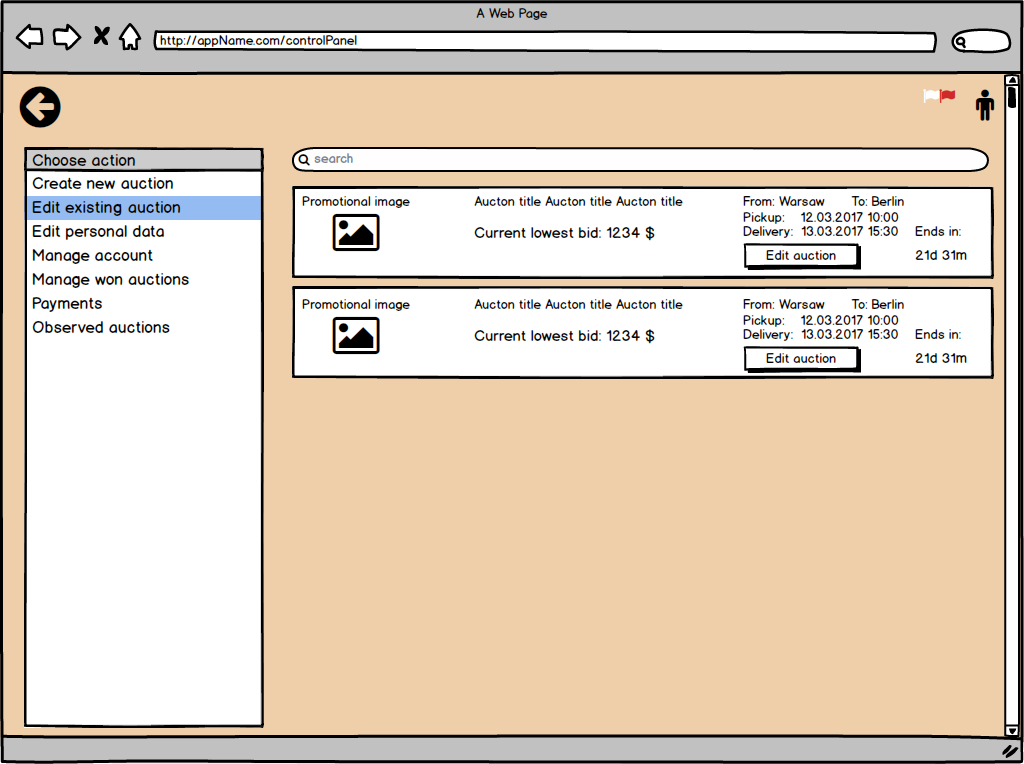
\includegraphics[width=\textwidth]{img/sekcja2/userPanelMock}
\caption[Szkice aplikacji - panel użytkownika]{Szkice aplikacji - panel użytkownika}
\end{figure}

\paragraph{Funkcjonalność}\mbox{}\\
Strona ta umożliwia zalogowanemu użytkownikowi zarządzanie swoim kontem oraz własnymi aukcjami.
\paragraph{Walidacja}\mbox{}\\
\begin{enumerate}[1.]
\item do wejścia na stronę wymagane jest zalogowanie się (aktywny token).
\end{enumerate}

%%%%%%%%%%%%%%%%%%%%%%%%%%%%%%%%%%%%%%%%%%%%%%%%%%%%%%%%%%%%%%%%%%%%%%%%
%%%%%%%%%%%%%%%%%%%%%%%%%%%%%%%%%%%%%%%%%%%%%%%%%%%%%%%%%%%%%%%%%%%%%%%%

\subsubsection{Aukcja}
\begin{figure}[H]
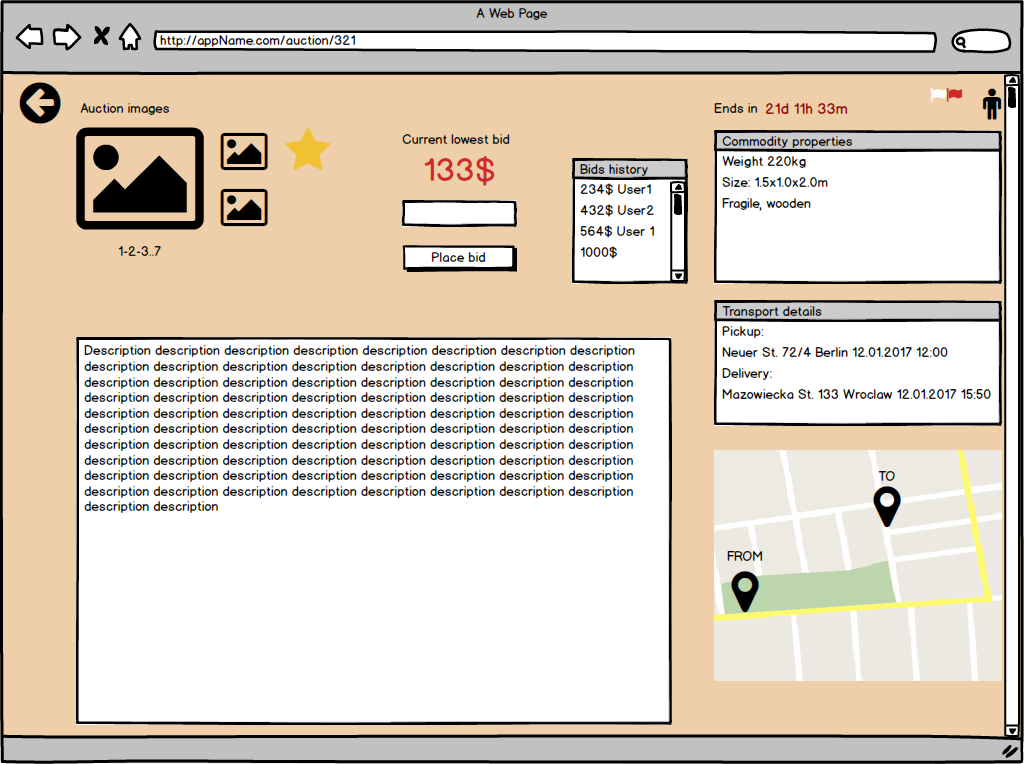
\includegraphics[width=\textwidth]{img/sekcja2/auctionMock}
\caption[Szkice aplikacji - aukcja]{Szkice aplikacji - aukcja}
\end{figure}

\paragraph{Funkcjonalność}\mbox{}\\
Strona ta pozwala zobaczyć treść konkretnej aukcji oraz złożyć swoją ofertę.
\paragraph{Walidacja}\mbox{}\\
\begin{enumerate}[1.]
\item Pole tekstowe: Przyjmuje jedynie cyfry, oraz znak przecinka bądź kropki. Maksimum znaków 15. 
\item Przycisk złóż ofertę: wymagane jest zalogowanie. Nowa oferta nie może być większa od aktualnej najmniejszej.
\end{enumerate}

%%%%%%%%%%%%%%%%%%%%%%%%%%%%%%%%%%%%%%%%%%%%%%%%%%%%%%%%%%%%%%%%%%%%%%%%
%%%%%%%%%%%%%%%%%%%%%%%%%%%%%%%%%%%%%%%%%%%%%%%%%%%%%%%%%%%%%%%%%%%%%%%%

\subsubsection{Stwórz nową aukcję}
\begin{figure}[H]
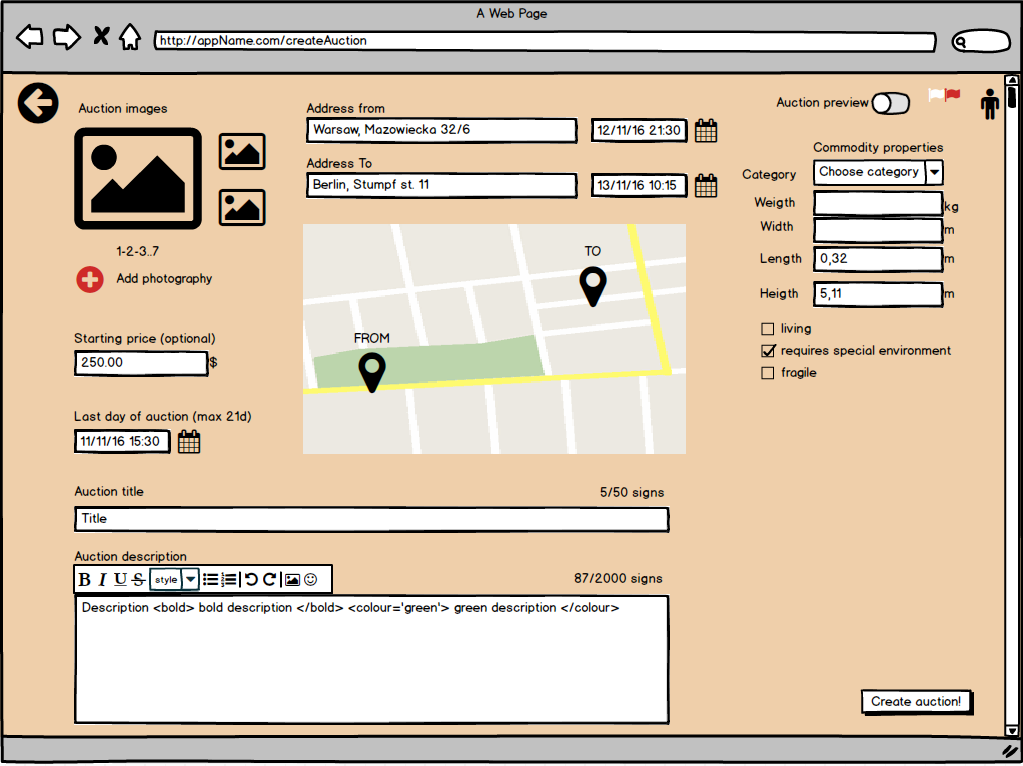
\includegraphics[width=\textwidth]{img/sekcja2/createAuctionMock}
\caption[Szkice aplikacji - stwórz nową aukcję]{Szkice aplikacji - stwórz nową aukcję}
\end{figure}

\paragraph{Funkcjonalność}\mbox{}\\
Strona ta pozwala na stworzenie nowej aukcji użytkownika. Pole tekstowe dotyczące opisu jest dynamicznie rozwijalne wraz z widocznym tekstem. Opis charakterystyki przedmiotu jest tylko przykładowy, dodatkowe parametry powinny zostać tutaj dodane. Po kliknięciu przycisku dodaj zdjęcie powinno wyskoczyć okienko z możliwością pobrania zdjęcia z dysku bądź z adresu internetowego.
\paragraph{Walidacja}\mbox{}\\
\begin{enumerate}[1.]
\item Pole tekstowe adresów: Adres będzie sprawdzany informacją zwrotną z \textit{Google Maps API}. Jeśli mapa poprawnie wykryje adres, to znaczy, że jest on prawidłowy. Maksimum znaków 50. 
\item Kalendarz: Data do i data od. Kalendarz pierwszej daty nie może być mniejszy od aktualnego dnia, ani daty dostarczenia towaru.
\item Pole tekstowe ceny początkowej: przyjmuje tylko cyfry, przecinek bądź kropkę. Maksimum znaków 15.
\item Pole tekstowe tytułu aukcji: walidacja słownikowa - zabronione hasła, niekulturalne wyrazy. Maksimum 50 znaków, minimum 5.
\item Pole tekstowe opisu aukcji: walidacja HTML, JavaScript, słownikowa. Maksymalnie 2000 znaków, łącznie ze znakami dostępnego kodu HTML.
\item Pole tekstowe dotyczące wagi oraz metrażu: maksymalnie dwa znaki po przecinku oraz ogólnie 9 znaków. Przyjmuje przecinek bądź kropkę.
\item Przycisk stwórz aukcję: wypełnione wszystkie wymagane pola.
\end{enumerate}
%%%%%%%%%%%%%%%%%%%%%%%%%%%%%%%%%%%%%%%%%%%%%%%%%%%%%%%%%%%%%%%%%%%%%%%%
%%%%%%%%%%%%%%%%%%%%%%%%%%%%%%%%%%%%%%%%%%%%%%%%%%%%%%%%%%%%%%%%%%%%%%%%

\subsubsection{Aktywacja konta}
\begin{figure}[H]
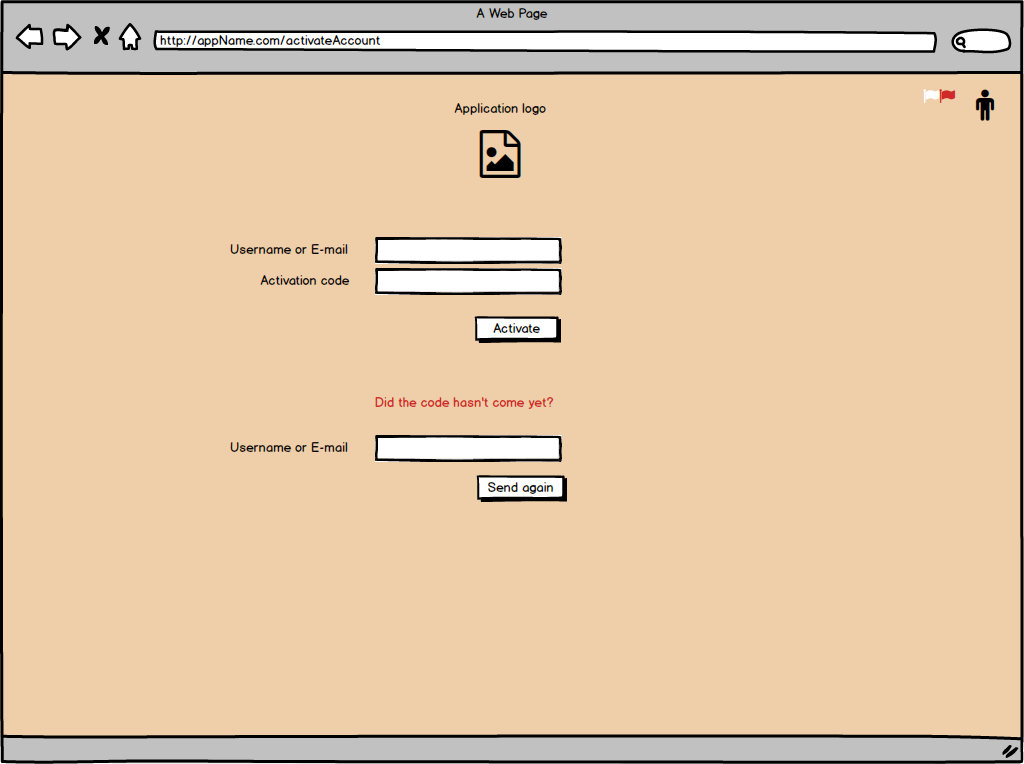
\includegraphics[width=\textwidth]{img/sekcja2/activateAccountMock}
\caption[Szkice aplikacji - aktywacja konta]{Szkice aplikacji - aktywacja konta}
\end{figure}

\paragraph{Funkcjonalność}\mbox{}\\
Strona umożliwia aktywacje nowego konta za pomocą kodu przysłanego na podany wcześniej adres e-mail.
\paragraph{Walidacja}\mbox{}\\
\begin{enumerate}[1.]
\item Pola tekstowe: brak
\end{enumerate}
%%%%%%%%%%%%%%%%%%%%%%%%%%%%%%%%%%%%%%%%%%%%%%%%%%%%%%%%%%%%%%%%%%%%%%%%
%%%%%%%%%%%%%%%%%%%%%%%%%%%%%%%%%%%%%%%%%%%%%%%%%%%%%%%%%%%%%%%%%%%%%%%%

\subsubsection{Wspólne elementy}
\begin{figure}[H]
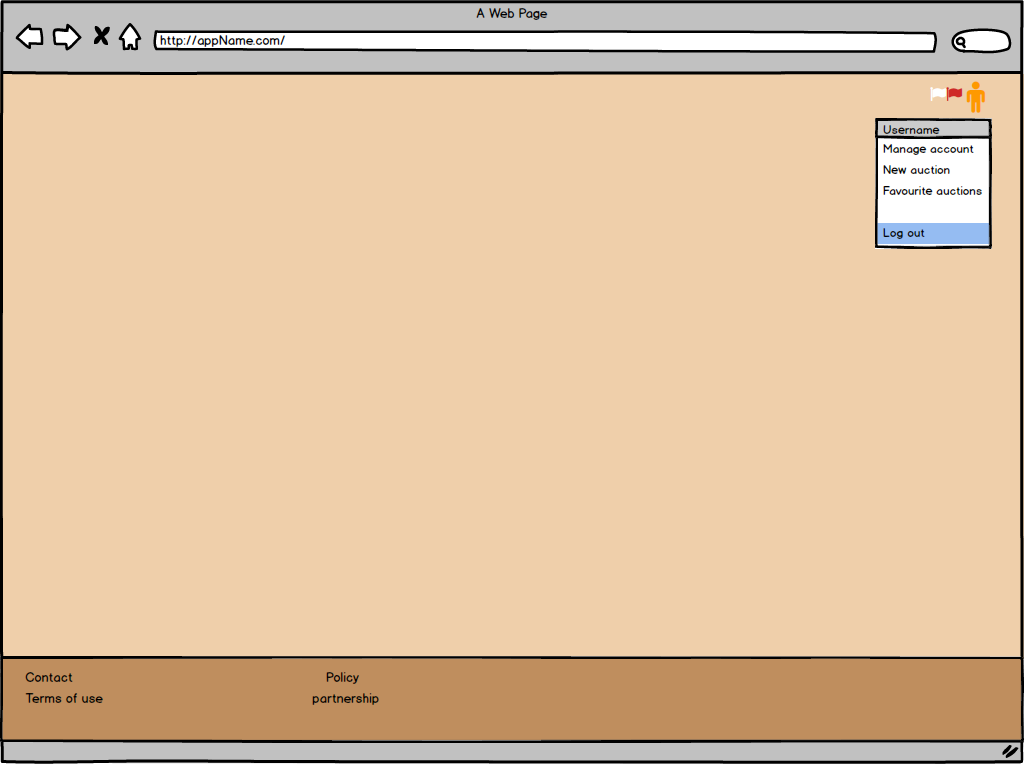
\includegraphics[width=\textwidth]{img/sekcja2/addidionalsMock}
\caption[Szkice aplikacji - wspólne elementy]{Szkice aplikacji - wspólne elementy}
\end{figure}

\paragraph{Funkcjonalność}\mbox{}\\
Na tym szkicu pokazane są wszystkie dodatkowe elementy wspólne, które pojawiają się na wszystkich innych podstronach.
\paragraph{Objaśnienia}\mbox{}\\
\begin{enumerate}[1.]
\item Ludzik: oznacza skrót do zarządzania kontem zalogowanego użytkownika. Dostępny jest jedynie po zalogowaniu. Przy kliknięciu ma pokazać listę szybkiego wyboru najczęściej używanych funkcjonalności.
\item Flagi: oznaczają aktualnie wyświetlany język. Po kliknięciu na flagę oznaczającą język konkretnego państwa, wszystkie wyświetlane elementy strony, zawierające tekst, mają się przeładować  na kliknięty język.
\item Stopka: Stopka jest niewielkim, statycznym elementem strony na samym dole, który będzie zawierać informacje handlowe, kontakt, warunki użycia aplikacji itp.
\end{enumerate}
%%%%%%%%%%%%%%%%%%%%%%%%%%%%%%%%%%%%%%%%%%%%%%%%%%%%%%%%%%%%%%%%%%%%%%%%
%%%%%%%%%%%%%%%%%%%%%%%%%%%%%%%%%%%%%%%%%%%%%%%%%%%%%%%%%%%%%%%%%%%%%%%%
%%%%%%%%%%%%%%%%%%%%%%%%%%%%%%%%%%%%%%%%%%%%%%%%%%%%%%%%%%%%%%%%%%%%%%%%
%%%%%%%%%%%%%%%%%%%%%%%%%%%%%%%%%%%%%%%%%%%%%%%%%%%%%%%%%%%%%%%%%%%%%%%%

\newpage
\section{Implementacja systemu}
\subsection{Implementacja bazy danych}
Implementacja bazy danych jest mocno powiązana z serwerem napisanym w języku \textit{Java}, dlatego też poniższe przykłady uwzględniają wycinki kodu z aplikacji.
Zaprojektowany, a później wgrany na bazę danych, projekt modelu baz danych, za pomocą programu \textit{IntelliJ} został przekonwertowany na odpowiednik klas Java przy wsparciu podstawowego standardu \textit{Java - JPA}. Niestety charakterystyka relacyjności nie została zachowana, dlatego też trzeba było napisać ją ręcznie, przy pomocy \textit{framework'a} \textit{Hibernate}. Narzędzie te realizuje za programistę chociażby problem mapowania obiektów. Dodatkowo posiada on wsparcie wielu rozszerzeń, tzw. \textit{toolboxów}, np. \textit{Hibernate Search}, ułatwiające implementacje systemu wyszukiwującego interesujące nas dane przy uwzględnieniu różnych parametrów.\mbox{}\\
Korzyści korzystania z \textit{framework'a} \textit{Hibernate} są dopiero widoczne dla średnich i większych aplikacji. Czas konfiguracji (encji i framework'u) dla małych aplikacji jest niewspółmierny do odniesionych korzyści.\mbox{}\\
W nawiasach podane zostały programy z których zostały zrobione powyższe zdjęcia.

\begin{figure}[H]%
    \centering
    \subfloat[Widok SQL (MySQL Workbench)]{{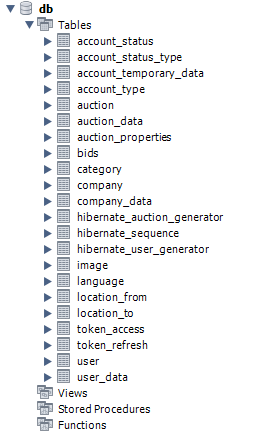
\includegraphics[width=0.47\textwidth, height=1.0\textheight, keepaspectratio ]{img/sekcja3/bd/bazaDanychWidokMySQL} }}%
    \qquad
    \subfloat[Widok Java (IntelliJ)]{{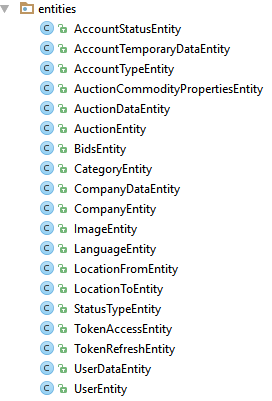
\includegraphics[width=0.47\textwidth, height=1.0\textheight, keepaspectratio]{img/sekcja3/bd/bazaDanychWidokJava} }}%
        \caption[Implementacja bazy danych - porównanie widoku bazy Java - SQL]{Implementacja bazy danych - porównanie widoku bazy Java - MySQL}%
\end{figure}
Powyższe rysunki pokazują różnicę w widoku bazy danych pomiędzy klasami \textit{Javy}, a encjami wygenerowanymi w języku \textit{SQL} poprzez te klasy. Różnica ilościowa widocznych encji wynika z tego, iż \textit{Hibernate} tworzy dodatkowe, pomocnicze, encje do obsługi danych, np. encja \textit{"hibernate\_auction\_generator"} używana jest do przechowywania ostatniego stworzonego numeru identyfikacyjnego aukcji.

\begin{figure}[H]%
    \centering
    \subfloat[Widok SQL (MySQL Workbench)]{{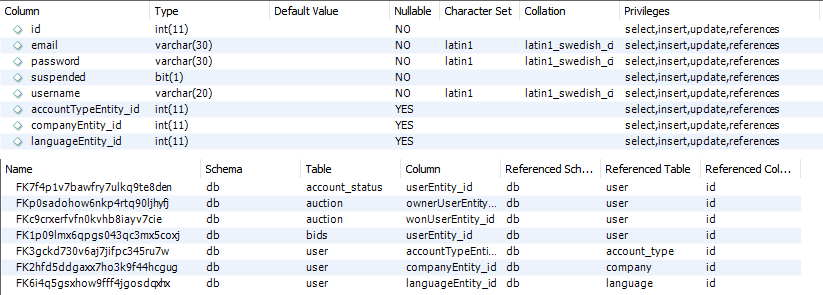
\includegraphics[width=1.0\textwidth, height=1.0\textheight, keepaspectratio ]{img/sekcja3/bd/encjaUserSQL} }}%
    \qquad
    \subfloat[Widok Java (IntelliJ)]{{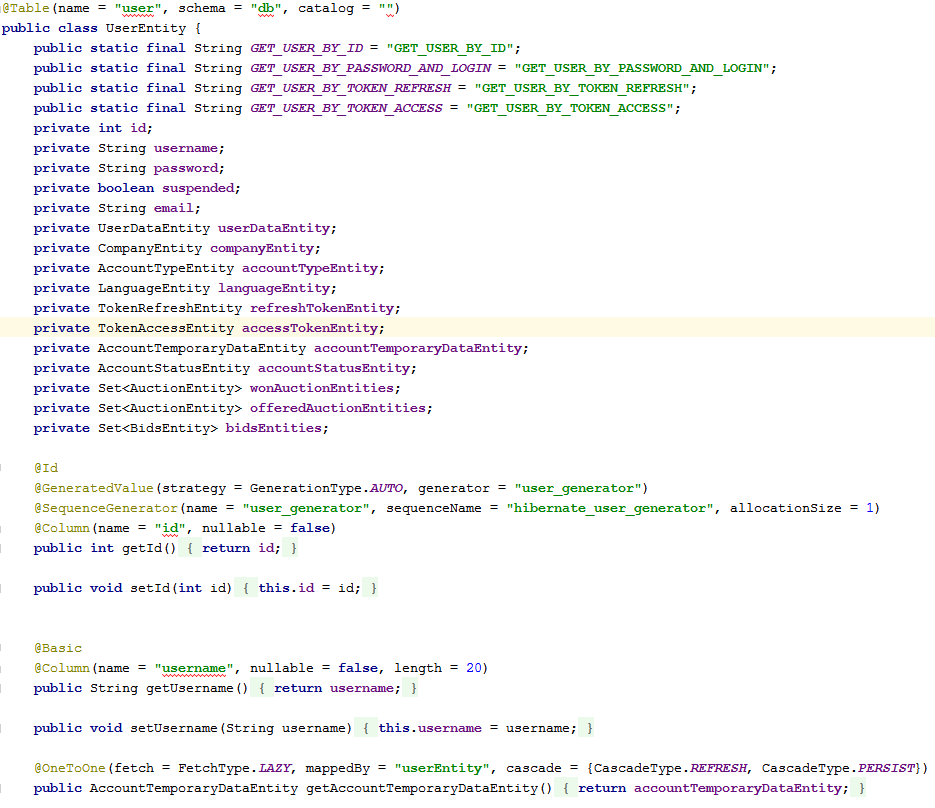
\includegraphics[width=1.0\textwidth, height=1.0\textheight, keepaspectratio]{img/sekcja3/bd/encjaUserJava} }}% 
     \caption[Implementacja bazy danych - porównanie widoku encji Java - SQL]{Implementacja bazy danych - porównanie widoku encji Java - MySQL}%
\end{figure}

Powyższe rysunki pokazują różnice widoku i implementacji danych pomiędzy encją napisaną w języku \textit{Java}, a \textit{SQL}. Szczegółowe objaśnienie zastosowanych rozwiązań encji napisanej w języku \textit{Java} zostało opisane w dziale \hyperref[Encje]{Implementacja serwera - Encje}.

\begin{listing}[H]
\caption[Konfiguracja dostępu do bazy danych przy użyciu \textit{Hibernate} - XML]{Konfiguracja dostępu do bazy danych przy użyciu \textit{Hibernate} - XML}
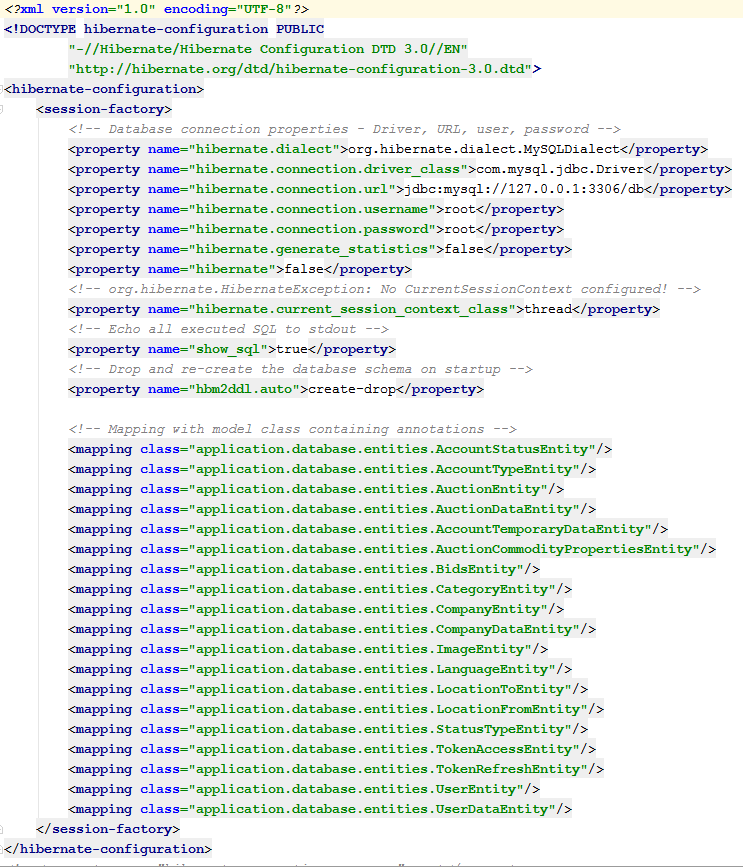
\includegraphics[width=1.0\textwidth, height=1.0\textheight, keepaspectratio]{img/sekcja3/bd/hibernateKonfiguracjaXML}
\end{listing}

\begin{listing}[H]
\caption[Konfiguracja dostępu do bazy danych przy użyciu \textit{Hibernate} - Java]{Konfiguracja dostępu do bazy danych przy użyciu \textit{Hibernate} - Java}
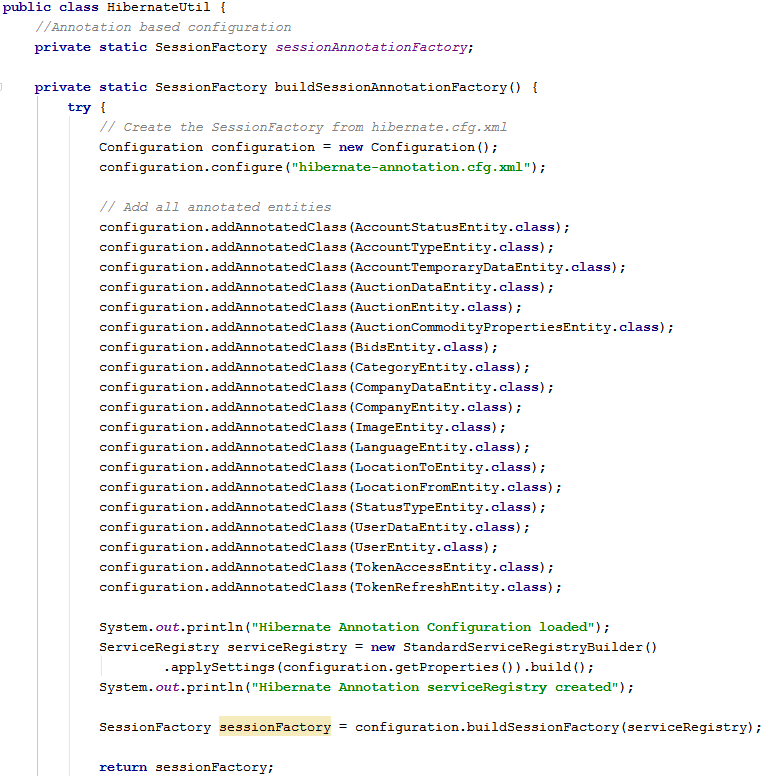
\includegraphics[width=1.0\textwidth, height=1.0\textheight, keepaspectratio ]{img/sekcja3/bd/hibernateKonfiguracjaJava}
\end{listing}
Główna konfiguracja ukryta jest w pliku \textit{XML}, która jest ładowana do konfiguracji napisanej w \textit{Javie}. Klasa ta tworzy instancje obiektu \textit{SessionFactory}, która odpowiedzialna jest za wszystkie czynności związane z komunikacją pomiędzy bazą danych, a Javą (np. zawieranie transakcji i dodawanie nowego obiektu).\mbox{}\\
Wykorzystanie klasy \textit{SessionFactory} jest bardziej szczegółowo opisane w dziale \hyperref[Obiekty dostępu danych - DAO]{obiekty dostępu danych - DAO}.
%%%%%%%%%%%%%%%%%%%%%%%%%%%%%%%%%%%%%%%%%%%%%%%%%%%%%%%%%%%%%%%%%%%%%%%%
%%%%%%%%%%%%%%%%%%%%%%%%%%%%%%%%%%%%%%%%%%%%%%%%%%%%%%%%%%%%%%%%%%%%%%%%
\subsection{Implementacja serwera}
\subsubsection{Struktura projektu}
\begin{figure}[H]
\centerline{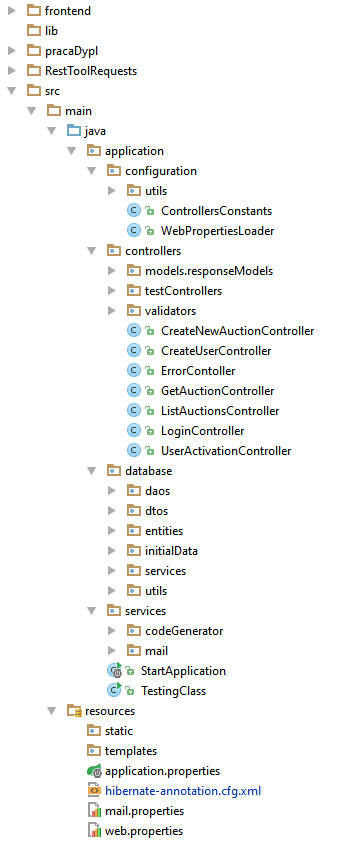
\includegraphics[height=0.85\textheight, keepaspectratio]{img/sekcja3/backend/strukturaProjektu}}
\caption[Implementacja serwera - struktura projektu]{Implementacja serwera - struktura projektu}
\end{figure} 
Powyżej została przedstawiona struktura widoczna jest z poziomu projektu serwera aplikacji. Widać na niej hierarchię wszystkich klas oraz wyraźny podział funkcjonalności pomiędzy bazę danych, a logikę biznesową.

%%%%%%%%%%%%%%%%%%%%%%%%%%%%%%%%%%%%%%%%%%%%%%%%%%%%%%%%%%%%%%%%%%%%%%%%
%%%%%%%%%%%%%%%%%%%%%%%%%%%%%%%%%%%%%%%%%%%%%%%%%%%%%%%%%%%%%%%%%%%%%%%%

\subsubsection{Konfiguracja projektu - Maven}
Konfiguracja zależności (używanych bibliotek i ich wersji) jest utrzymywana przy pomocy \textit{framework'u} \textit{Maven} w pliku \textit{pom.xml}. Jest to bardzo prosty sposób utrzymywania projektu, ponieważ, aby zainstalować projekt na innym komputerze, należy jedynie użyć komendy \textit{mvn clean install} w terminalu konsoli, będąc w katalogu z projektem.
\begin{listing}[H]
\caption[Implementacja serwera - konfiguracja \textit{Maven'a} ]{Implementacja serwera - konfiguracja \textit{Maven'a}}
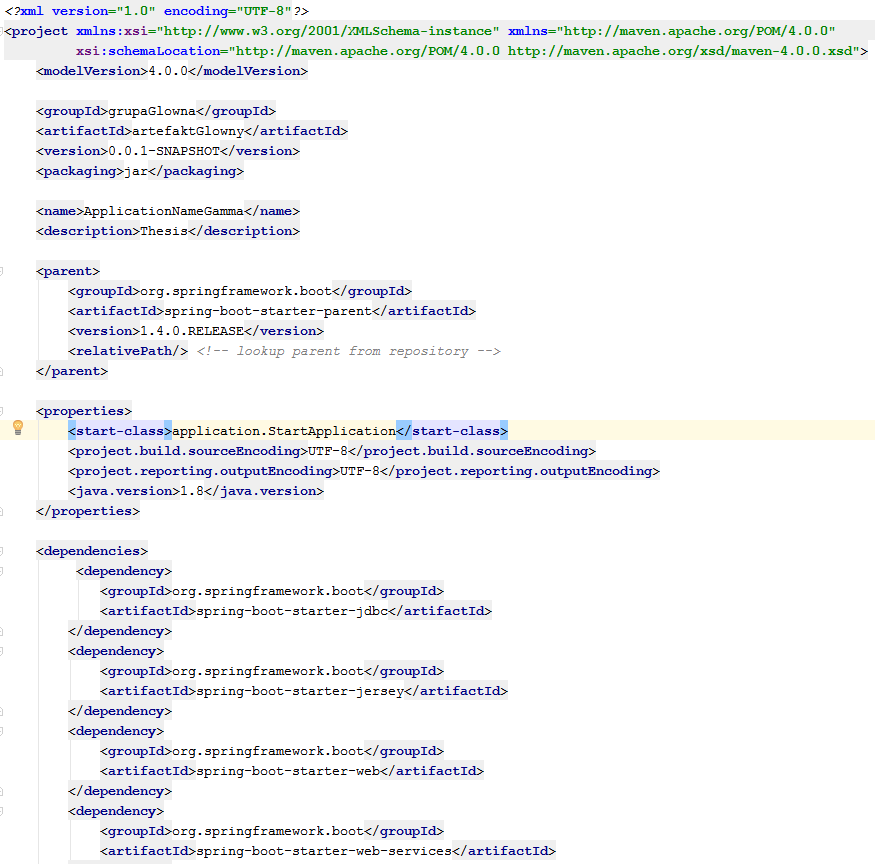
\includegraphics[width=1.0\textwidth, height=0.85\textheight ]{img/sekcja3/backend/konfiguracjaMaven}
\end{listing} 

%%%%%%%%%%%%%%%%%%%%%%%%%%%%%%%%%%%%%%%%%%%%%%%%%%%%%%%%%%%%%%%%%%%%%%%%
%%%%%%%%%%%%%%%%%%%%%%%%%%%%%%%%%%%%%%%%%%%%%%%%%%%%%%%%%%%%%%%%%%%%%%%%

\subsubsection{Encje}\label{Encje}

\begin{listing}[H]
\caption[Implementacja serwera - encje]{Implementacja serwera - encje}
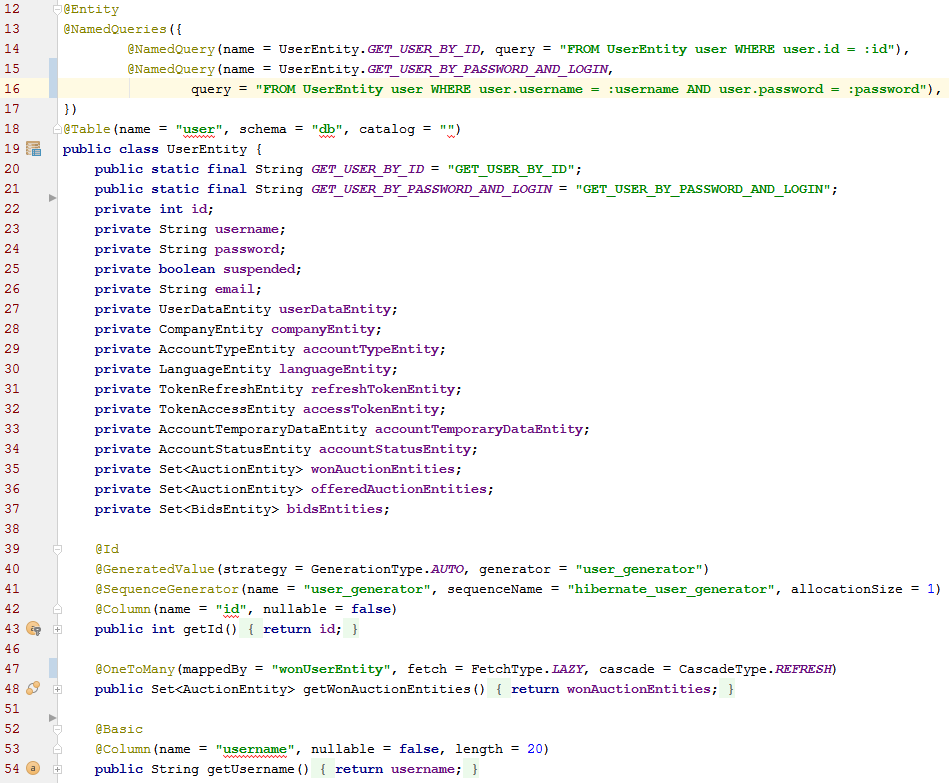
\includegraphics[width=1.0\textwidth, height=0.85\textheight]{img/sekcja3/backend/encjaUzytkownik}
\end{listing} 

Powyższy przykład pokazuje przykładową encję napisaną w języku Java (została uproszczona względem aktualnej), używającej rozwiązania z \textit{framework'u} \textit{Hibernate} oraz standardowej biblioteki \textit{JPA} służące do modelowania obiektów oraz rozwiązujących za nas problem mapowania obiektów.
\textit{Hibernate} umożliwia nam także korzystanie z definiowanych zapytań które są napisane w specjalnym języku wspieranym przez ten \textit{framework} - \textit{HQL - Hibernate Query Language} (są one widoczne przy adnotacji \textit{@NamedQueries - 13 linia}. Zapytania te nie różnią się specjalnie od zwykłych zapytań \textit{SQL}. Do oznaczenia tabeli używana jest adnotacja \textit{@Table - 18 linia} wraz z odpowiednimi argumentami.    Do generowania sekwencji identyfikatora rekordu, używany jest modyfikowalny \textit{@SequenceGenerator - 41 linia}. Dla każdej encji zalecane jest używanie własnego generatora (bądź, jeśli mamy encje jeden-do-jednego, wspólnego z encją rodzicem). W przypadku jednego generatora, każdy rekord będzie miał kolejny identyfikator, dzielony ze wszystkimi encjami. W \textit{47 linii} mamy przykład użycia relacji jeden-do-wielu między encją użytkownika (widoczną), a aukcji, gdzie encja użytkownika jest właścicielem relacji, (zawiera w sobie kolekcję obiektów \textit{Set<AuctionEntity> - linia 35} encji aukcji) co oznacza, że jeden użytkownik może posiadać 0 bądź wiele aukcji. Na samym dole mamy oznaczenie pola przy użyciu adnotacji \textit{@Basic oraz @Column}. Pierwsza z nich oznacza domyślną konfigurację pola, czyli czy pole jest opcjonalne oraz tryb wyciągania danych (\textit{fetch}) - gorliwy (\textit{eager}) czy leniwy (\textit{lazy}).

%%%%%%%%%%%%%%%%%%%%%%%%%%%%%%%%%%%%%%%%%%%%%%%%%%%%%%%%%%%%%%%%%%%%%%%%
%%%%%%%%%%%%%%%%%%%%%%%%%%%%%%%%%%%%%%%%%%%%%%%%%%%%%%%%%%%%%%%%%%%%%%%%
\subsubsection{Obiekty dostępu danych}\label{Obiekty dostępu danych - DAO}

\begin{listing}[H]
\caption[Implementacja serwera - wspólne metody]{Implementacja serwera - wspólne metody}
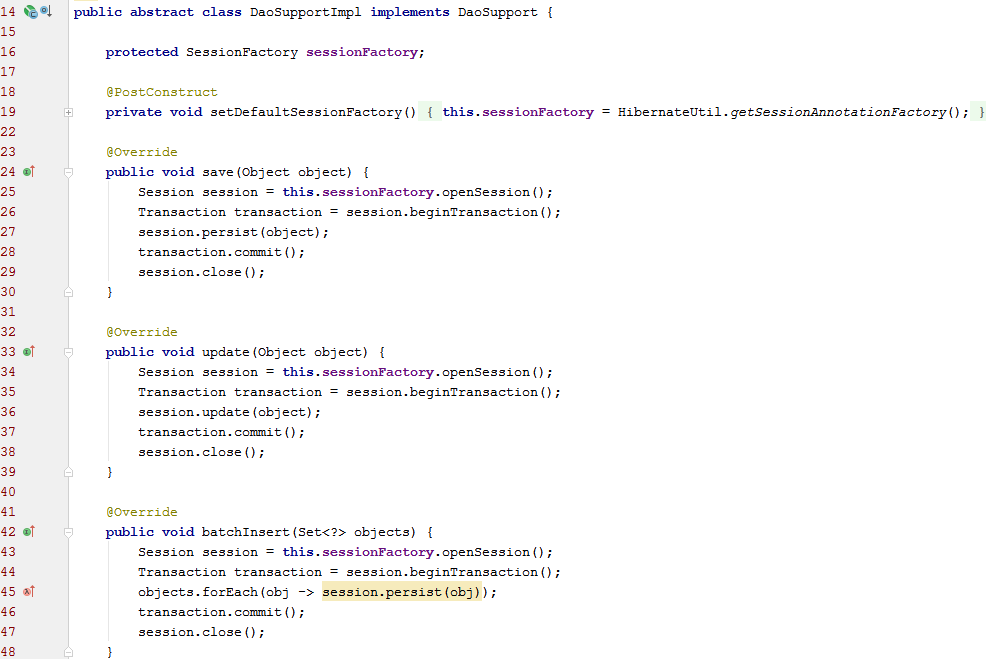
\includegraphics[width=1.0\textwidth, height=0.75\textheight]{img/sekcja3/backend/daoSupport}
\end{listing} 
Widoczne metody, są podstawowymi operacjami dostępnymi dla wszystkich obiektów dostępu danych (DAO - Data Access Object). Każda klasa typu \textit{DAO} dziedziczy po wyżej widocznej klasie.

\begin{listing}[H]
\caption[Implementacja serwera - obiekt dostępu danych użytkownika]{Implementacja serwera - obiekt dostępu danych użytkownika}
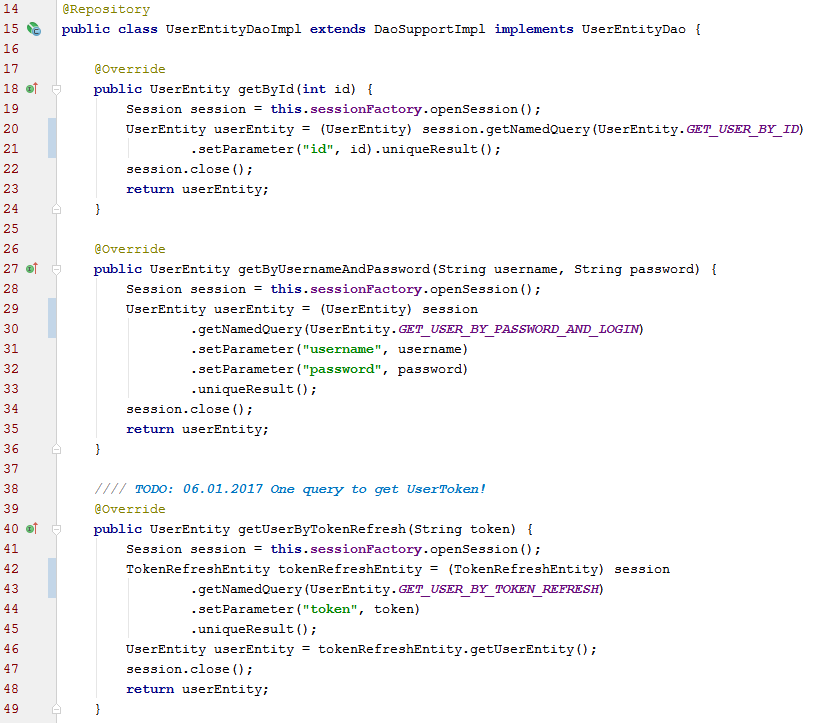
\includegraphics[width=1.0\textwidth, height=0.85\textheight]{img/sekcja3/backend/daoUzytkownik}
\end{listing} 

Powyższy przykład pokazuje przykładowy obiekt dostępu danych do bazy (został on uproszczony względem aktualnego). Używa on uprzednio skonfigurowanych obiektów typu \textit{org.hibernate.SessionFactory} które przechowują w sobie dane potrzebne do połączenia oraz narzędzia umożliwiające przesył informacji pomiędzy bazą danych, a aplikacją Javy.
Kod jest napisany bardzo schematycznie, na początku tworzymy sesje i w zależności czy potrzebujemy pobrać dane czy je zapisać zawieramy transakcję i potwierdzamy zmiany. Na samym końcu należy pamiętać o zamknięciu połączenia. 

%%%%%%%%%%%%%%%%%%%%%%%%%%%%%%%%%%%%%%%%%%%%%%%%%%%%%%%%%%%%%%%%%%%%%%%%
%%%%%%%%%%%%%%%%%%%%%%%%%%%%%%%%%%%%%%%%%%%%%%%%%%%%%%%%%%%%%%%%%%%%%%%%
\subsubsection{Serwisy danych}
Serwisy danych są odpowiedzialne za przetworzenie danych oraz udostępnienie jej aplikacji (serwisy danych) , bądź wystawienie na zewnątrz (np. serwis poczty elektronicznej) - posiadają większość logiki biznesowej.
\begin{listing}[H]
\caption[Implementacja serwera - serwis użytkownika]{Implementacja serwera - serwis użytkownika}
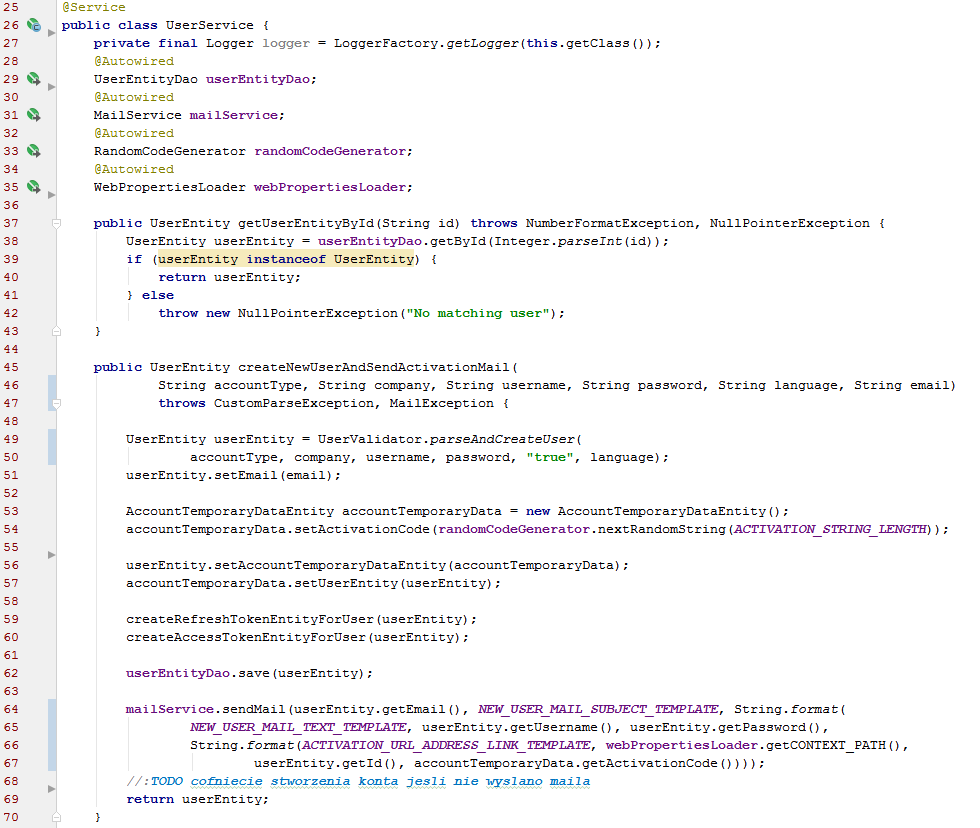
\includegraphics[width=1.0\textwidth, height=0.8\textheight]{img/sekcja3/backend/serwisUzytkownik}
\end{listing}
Jest to przykład serwisu danych używanego do wszystkich akcji związanych z użytkownikiem - większości w tej aplikacji. Przy \textit{37 oraz 45} widać dwie przykładowe metody, \textit{getUserEntityById} oraz \textit{createNewUserAndSendActivationMail}. Pierwsza z nich odpowiada za pobranie istniejącego użytkownika z bazy danych po unikatowym identyfikatorze, oraz przekazanie go. Druga tworzy nowego użytkownika oraz wysyła e-mail z kluczem i linkiem aktywacyjnym. Widać tutaj wcześniej opisane obiekty \textit{DAO - Data Access Object} np. klasę \textit{UserEntityDao - linia 29}. Obiekty te są zarządzane przez implementacje kontenera \textit{IoC - Inversion of Control} przez \textit{framework} \textit{Spring}. Kontener ten zarządza cyklem życia wszystkich oznaczonych dla niego obiektów. Szczegółowy opis tej implementacji można znaleźć na oficjalnej stronie dokumentacji \textit{framework'u} \href{https://docs.spring.io/spring/docs/current/spring-framework-reference/html/beans.html}{\textit{Spring}}\cite{ioc}. Przykładem takiego oznaczenia jest adnotacja \textit{@Service - 25 linia}, oznaczająca serwis danych. Wstrzykiwanie takiego obiektu oznacza się adnotacją \textit{@Autowired - 28, 30, 32, 34 linia}, z ewentualnym argumentem nazwy ziarenka (\textit{Bean}), jeśli jest ono inne od nazwy domyślnej (nazwy klasy).

%%%%%%%%%%%%%%%%%%%%%%%%%%%%%%%%%%%%%%%%%%%%%%%%%%%%%%%%%%%%%%%%%%%%%%%%
%%%%%%%%%%%%%%%%%%%%%%%%%%%%%%%%%%%%%%%%%%%%%%%%%%%%%%%%%%%%%%%%%%%%%%%%

\subsubsection{Serwis mailowy}

\begin{listing}[H]
\caption[Implementacja serwera - serwis e-mail]{Implementacja serwera - serwis e-mail}
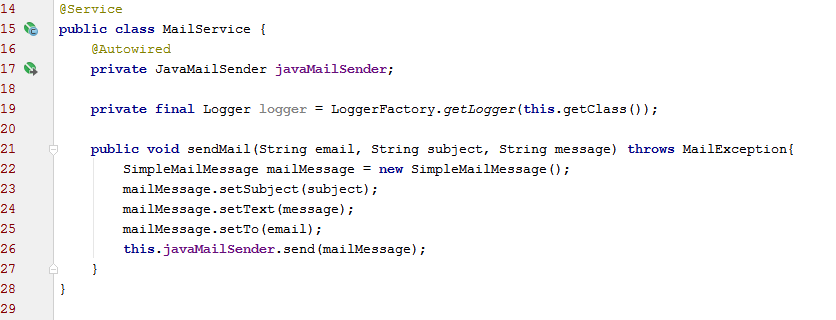
\includegraphics[scale=0.7]{img/sekcja3/backend/serwisMailowy}
\end{listing}
Implementacja serwisu mailowego używa już dostępnej klasy z pakietu \textit{Spring} i w związku z tym ogranicza się jedynie do wykorzystania już dostępnych funkcji widocznych na powyższym obrazku. Jedynym wymaganiem jest przekazanie skonfigurowanego obiektu który by e-maile wysyłał. Ten obiekt widoczny jest w \textit{17 linii - JavaMailSender}.

\begin{listing}[H]
\caption[Implementacja serwera - konfiguracja serwisu e-mail]{Implementacja serwera - konfiguracja serwisu e-mail}
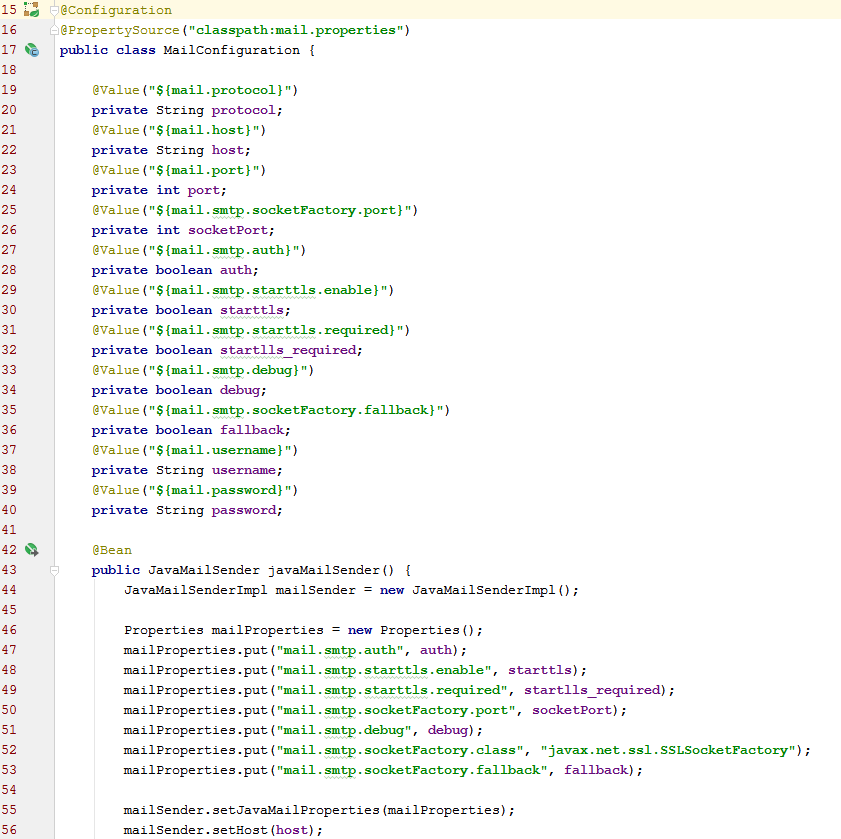
\includegraphics[width=1.0\textwidth, height=0.8\textheight]{img/sekcja3/backend/konfiguracjaSerwisuMailowego}
\end{listing}
Plik konfiguracyjny zarządzany przez kontener \textit{Spring} musi być widoczny dla niego. Najłatwiej osiągnąć można to używając adnotacji \textit{@Configuration - linia 15}. Adnotacja poniżej \textit{@PropertySource - linia 16} oznacza, iż dane będą wczytywane z zewnętrznego pliku (w tym przypadku pliku znajdującego się w katalogu z lokalnymi zasobami projektu (\textit{resources}). Aby wczytać poszczególne dane, używana jest adnotacja \textit{@Value(\${szukany ciąg znaków})}, która po szukanym ciągu znaków wczytuje wiersz danych. Przy użyciu wspólnie adnotacji \textit{@Configuration - linia 15 oraz @Bean - linia 42} można innym sposobem stworzyć obiekt (\textit{ziarenko - Bean}) zarządzane przez kontener \textit{Spring}. Widoczny skonfigurowany obiekt klasy \textit{JavaMailSender} jest wstrzykiwany w serwisie mailowym opisanym wyżej.

\begin{figure}[H]
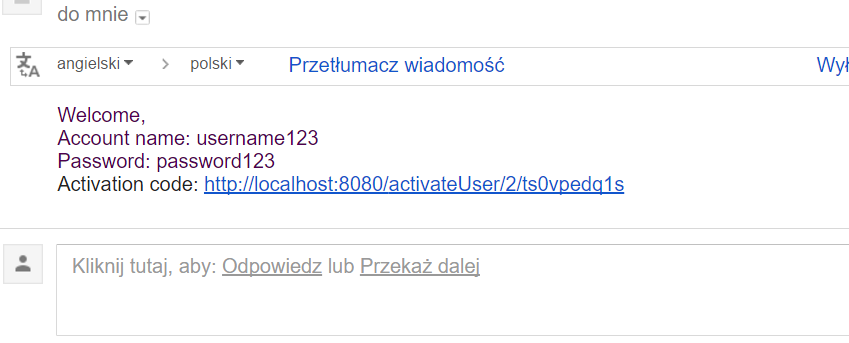
\includegraphics[width=\textwidth]{img/sekcja3/backend/przykladowyEmail}
\caption[Implementacja serwera - przykładowy e-mail]{Implementacja serwera - przykładowy e-mail}
\end{figure}
Powyżej widoczna jest przykładowa wiadomość aktywacykna użytkownika wysłana przez serwis e-mail. 

%%%%%%%%%%%%%%%%%%%%%%%%%%%%%%%%%%%%%%%%%%%%%%%%%%%%%%%%%%%%%%%%%%%%%%%%%%%%%%%%%%%%%%%%%%%%%%%%%%%%%%%%%%%%%%%%%%%%%%%%%%%%%%%%%%%%
\subsubsection{Udostępnianie danych za pomocą kontrolera}
Kontrolery mają za zadanie udostępnić dane na zewnątrz które są transportowane przy pomocy protokołów \textit{HTTP}, wykonując zapytanie z odpowiednimi argumentami oraz adresem strony.

\begin{listing}[H]
\caption[Implementacja serwera - kontroler tworzący nowego użytkownika]{Implementacja serwera - kontroler tworzący nowego użytkownika}
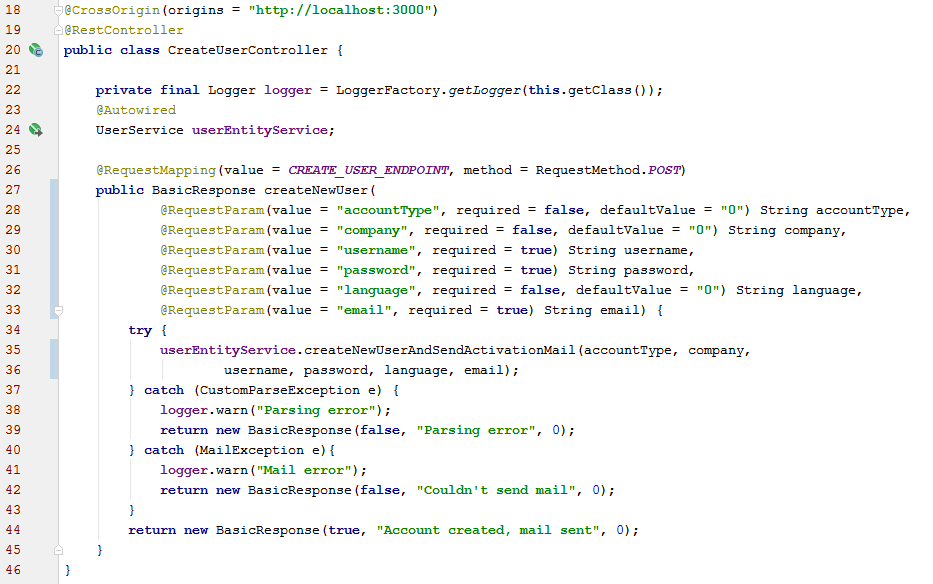
\includegraphics[width=1.0\textwidth, height=0.5\textheight]{img/sekcja3/backend/kontrolerUzytkownik}
\end{listing}

Powyższy przykład posiada wiele adnotacji, jednakże najważniejszymi z nich są \textit{@RequestMapping - 26 linia} którego argumentami jest nazwa \textit{endpointu} oraz metoda którą należy się odwoływać do niego, aby otrzymać prawidłową odpowiedź. Poniżej widoczna jest adnotacja \textit{@RequestParam - 27 do 32 linii} która odpowiada za przyjmowane argumenty przez \textit{endpoint}.
Dane zwracane poprzez ten \textit{endpoint} są automatycznie parsowane przez parser \textit{JSON} dzięki adnotacji \textit{@RestController - 19 linia}. 

%%%%%%%%%%%%%%%%%%%%%%%%%%%%%%%%%%%%%%%%%%%%%%%%%%%%%%%%%%%%%%%%%%%%%%%%
%%%%%%%%%%%%%%%%%%%%%%%%%%%%%%%%%%%%%%%%%%%%%%%%%%%%%%%%%%%%%%%%%%%%%%%%

\subsubsection{Przykładowe obiekty transferu danych - DTO}
Obiekty \textit{DTO - Data Transfer Object} są zwyczajnymi kontenerami na dane. Jednakże są one potrzebne, aby wystawiać informacje tylko te które chcemy. Jeśli udostępnialibyśmy obiekty reprezentujące encje bazodanowe mogłoby to zrodzić sytuację kiedy to parser JSON'owy wystawiłby niepożądane informacje takie jak w przypadku aukcji - hasło, login, oraz wszystkie szczegółowe informacje użytkowników mających zależności z daną aukcją (licytujący, właściciel aukcji).

\begin{listing}[H]
\caption[Implementacja serwera - przykładowy obiekt transferu danych - aukcja]{Implementacja serwera - przykładowy obiekt transferu danych - aukcja}
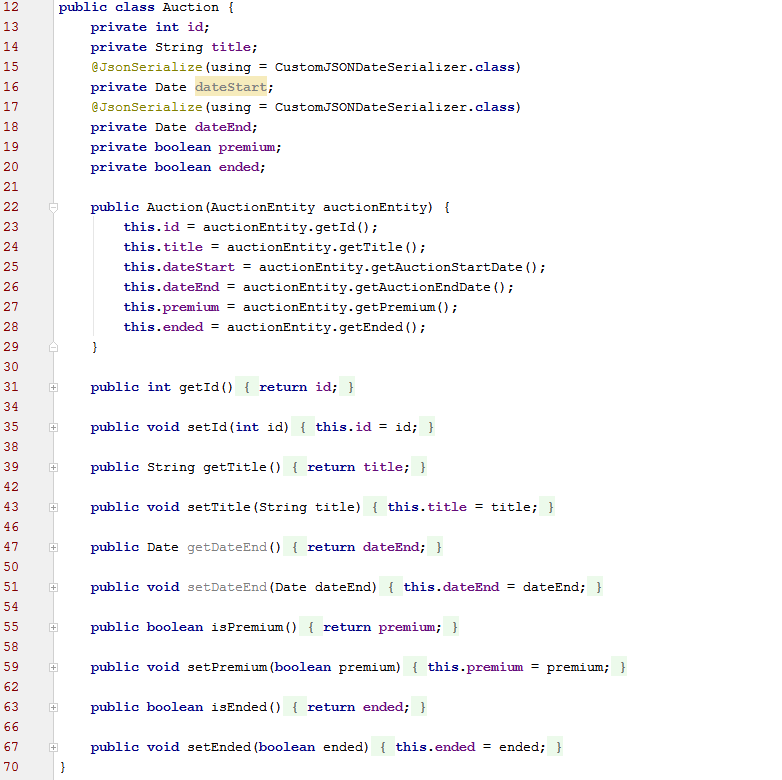
\includegraphics[width=\textwidth]{img/sekcja3/backend/dtoAuction}
\end{listing}
Na rysunku powyżej widoczny jest klasyczny przykład obiektu \textit{DTO}. Posiada on konstruktor używający encji \textit{AuctionEntity - linia 22} do zapełnienia pól. Takie rozwiązanie umożliwia pokazanie wybranych danych. Dodatkowo adnotacja \textit{JsonSerialize - linia 15 i 17} oznacza, iż używamy własnej implementacji serializatora \textit{JSON} zamiast domyślnej do parsowania obiektu. \textit{Gettery i Settery} są wymagane przez każdy serializator \textit{JSON}, aby dostać się do konkretnych pól, ponieważ używa on mechanizmu refleksji klas, aby dowiedzieć się jakie pola posiada serializowany obiekt i na ich podstawie próbuje dostać się do danych.

%%%%%%%%%%%%%%%%%%%%%%%%%%%%%%%%%%%%%%%%%%%%%%%%%%%%%%%%%%%%%%%%%%%%%%%%
%%%%%%%%%%%%%%%%%%%%%%%%%%%%%%%%%%%%%%%%%%%%%%%%%%%%%%%%%%%%%%%%%%%%%%%%

\subsubsection{Dane inicjujące}
Dane inicjujące są zapisane w formie kodu \textit{Java} za pomocą encji (zagnieżdżonych jeśli występują asocjacje).

\begin{listing}[H]
\caption[Implementacja serwera - przykładowy dane inicjujące]{Implementacja serwera - przykładowy dane inicjujące}
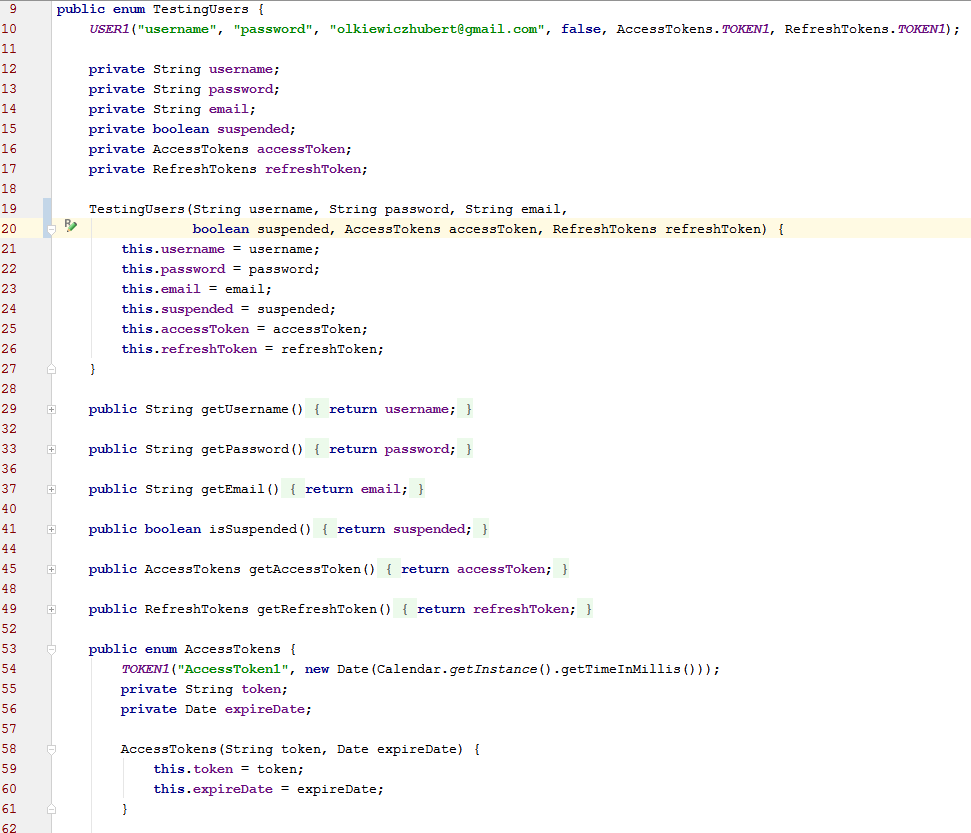
\includegraphics[width=1.0\textwidth, height=0.8\textheight]{img/sekcja3/backend/daneInicjalizacyjne}
\end{listing}

Powyższy przykład pokazuje jedną z takich klas - \textit{TestingUsers - użytkownicy testowi}. Widoczna jest dodatkowo zagnieżdżona encja posiadające dane o tokenach, potrzebna do testowania \textit{endpointów} serwera. Raz napisany mechanizm, pozwala bardzo łatwo i schematycznie, z poziomu kodu, dodawać nowe rekordy do testowania aplikacji. Wystarczy według wzoru wstawiać odpowiednie dane tak jak w \textit{10 linii} kodu.
%%%%%%%%%%%%%%%%%%%%%%%%%%%%%%%%%%%%%%%%%%%%%%%%%%%%%%%%%%%%%%%%%%%%%%%%
%%%%%%%%%%%%%%%%%%%%%%%%%%%%%%%%%%%%%%%%%%%%%%%%%%%%%%%%%%%%%%%%%%%%%%%%

\subsubsection{Przykład uruchomienia serwera}
\textit{Spring} za nas zajmuje się całą konfiguracją sieciową oraz serwerem aplikacji internetowych (\textit{Tomcat}) na którym instalowany jest nasz napisany program.

\begin{listing}[H]
\centering
\caption[Implementacja serwera - klasa uruchomiająca]{Implementacja serwera -  klasa uruchomiająca}
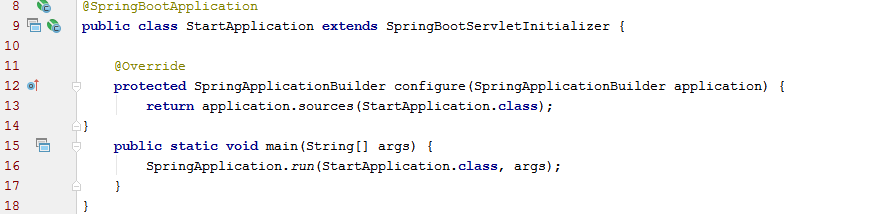
\includegraphics[width=\textwidth]{img/sekcja3/backend/klasaStartowa}
\end{listing}

Aby uruchomić naszą aplikację należy zwyczajnie uruchomić ją z klasy \textit{StartApplication - 9 linia}, \textit{metoda main(String[] args) - 15 linia}. Klasa ta jest bardzo schematycznie napisana, wymagana jest adnotacja \textit{SpringBootApplication - 8 linia} oraz rozszerzenie o klasę \textit{SpringBootServletInitializer - 9 linia}, która posiada metodę \textit{configure - 12} konfiguracyjną, którą należy nadpisać.

\begin{figure}[H]
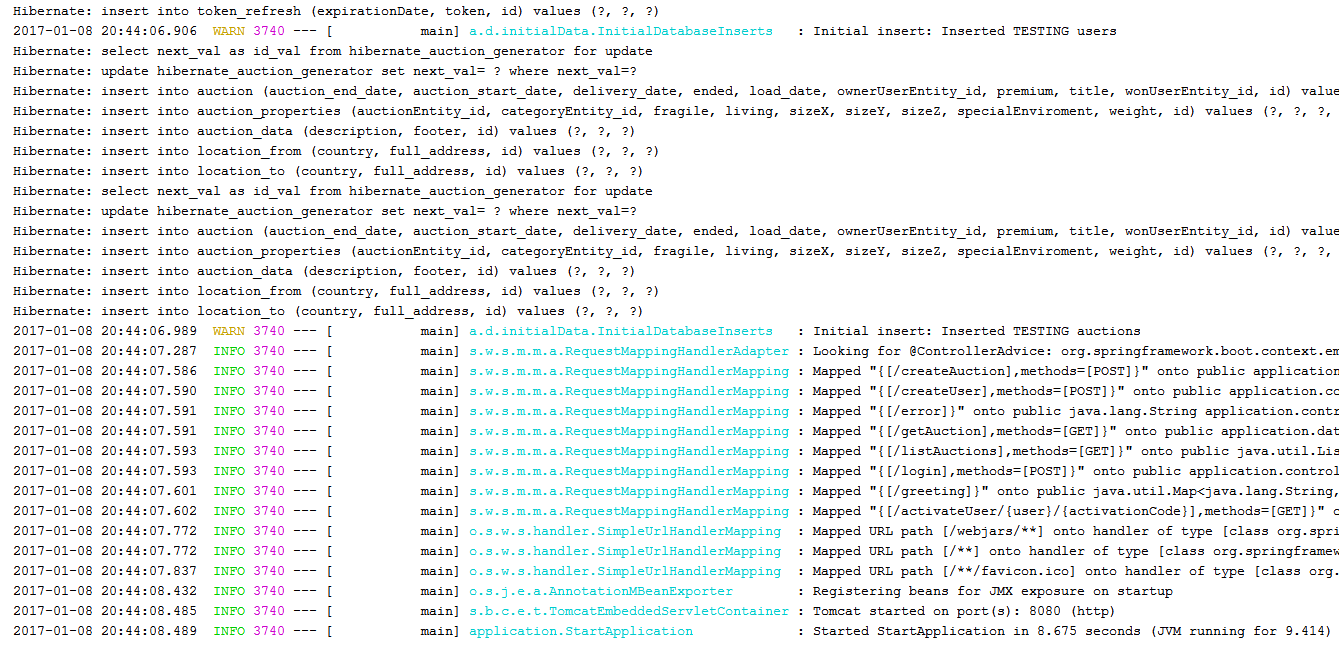
\includegraphics[width=1.0\textwidth, height=0.5\textheight]{img/sekcja3/backend/uruchomienieSerwera}
\caption[Wyciąg z konsoli po uruchomieniu serwera]{Wyciąg z konsoli po uruchomieniu serwera}
\end{figure}

Powyższe zdjęcie pokazuję kawałek wypisanych informacji przy uruchomieniu aplikacji (z klasy opisanej zdjęcie wyżej). Widać na nim fragmenty kodu \textit{HQL - Hibernate Query Language} inicjujące bazę danych oraz konfigurację \textit{endpointów} naszej aplikacji i port na który można się do nich odwoływać.

%%%%%%%%%%%%%%%%%%%%%%%%%%%%%%%%%%%%%%%%%%%%%%%%%%%%%%%%%%%%%%%%%%%%%%%%
%%%%%%%%%%%%%%%%%%%%%%%%%%%%%%%%%%%%%%%%%%%%%%%%%%%%%%%%%%%%%%%%%%%%%%%%
%%%%%%%%%%%%%%%%%%%%%%%%%%%%%%%%%%%%%%%%%%%%%%%%%%%%%%%%%%%%%%%%%%%%%%%%
%%%%%%%%%%%%%%%%%%%%%%%%%%%%%%%%%%%%%%%%%%%%%%%%%%%%%%%%%%%%%%%%%%%%%%%%


\subsection{Implementacja aplikacji klienckiej}
Aplikacja kliencka jest zintegrowana z \textit{serwerem backendowym}, jednakże nie jest ona jeszcze dopracowana. Większość szablonów projektowych zostało zaimplementowanych. Niestety nie starczyło czasu na upiększenie jej za pomocą odpowiednich znaczników języka \textit{HTML} oraz \textit{CSS}.

\subsubsection{Struktura projektu}
\begin{figure}[H]
\centering
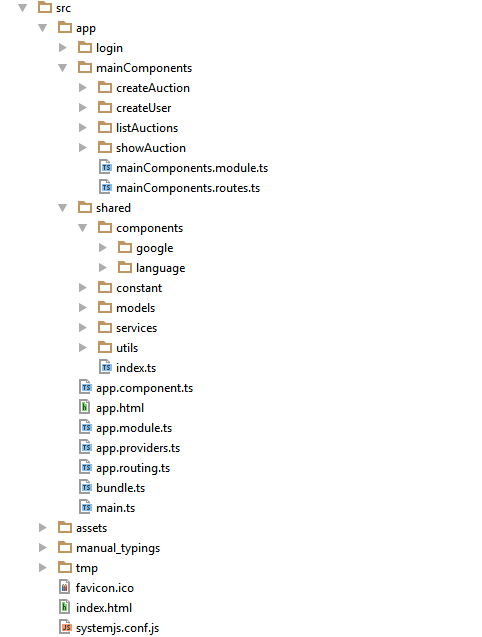
\includegraphics[scale=0.75]{img/sekcja3/frontend/strukturaProjektu}
\caption[Implementacja aplikacji klienckiej - struktura projektu]{Implementacja aplikacji klienckiej - struktura projektu}
\end{figure}

Powyżej widoczna jest struktura projektu (z poziomu programu \textit{WebStorm}). \textit{Angular2} stawia na modułowość, przez co jest podobny do języków obiektowych takich jak \textit{Java} czy \textit{\texttt{C\#}}. Głównym modułem z aplikacji są klasy zaczynające się od nazwy \textit{app.} (szczegółowo opisane w rozdziale \hyperref[Glowny modul aplikacji]{główny moduł aplikacji}). Od nich zaczyna się główny program, który ładuje pozostałe moduły (np. \textit{mainComponents} - główne komponenty odpowiedzialne za pokazanie aukcji czy stworzenie użytkownika). 
%%%%%%%%%%%%%%%%%%%%%%%%%%%%%%%%%%%%%%%%%%%%%%%%%%%%%%%%%%%%%%%%%%%%%%%%
%%%%%%%%%%%%%%%%%%%%%%%%%%%%%%%%%%%%%%%%%%%%%%%%%%%%%%%%%%%%%%%%%%%%%%%%

\subsubsection{Integracja z serwerem}
\begin{listing}[H]
\caption[Implementacja aplikacji klienckiej - integracja z serwerem]{Implementacja aplikacji klienckiej - integracja z serwerem}
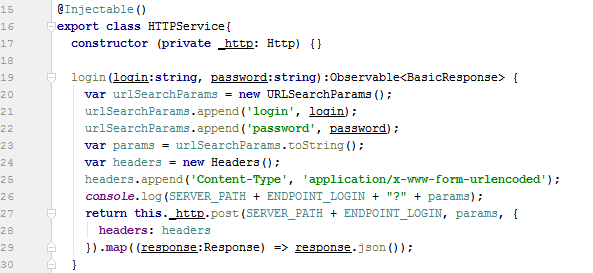
\includegraphics[width=\textwidth]{img/sekcja3/frontend/logowanieRequest}
\end{listing}

Powyżej widać przykład metody napisanej w języku \textit{TypeScript} przy użyciu rozwiązań z \textit{framework'a} \textit{Angular2} - moduł obsługujący zapytania \textit{HTTP}. Widoczna jest także zaimplementowana metoda logowania \textit{login - 19 linia}. Zwraca ona charakterystyczny dla tego języka typ danych - \textit{Observable} który pozwala "leniwie" załadować dane (np. ustawić czas oczekiwania na dane na 10 sekund i dopiero po nim pokazać błąd). Obiekt ten działa asynchronicznie względem reszty aplikacji - kiedy wywoływany, uruchamia się oddzielny wątek, wywłaszczający go i realizujący operacje na nim. Parametrami przy logowaniu są hasło oraz nazwa użytkownika, oraz opcjonalnie token. Jeśli token znajdzie się w zapytaniu do \textit{serwera backendowego}, wtedy pobierany jest, przy pozytywnym sprawdzeniu danych i tokena, token o podwyższonych uprawnieniach.

\begin{figure}[H]%
    \centering
    
    \subfloat[Zapytanie \textit{HTTP}]{{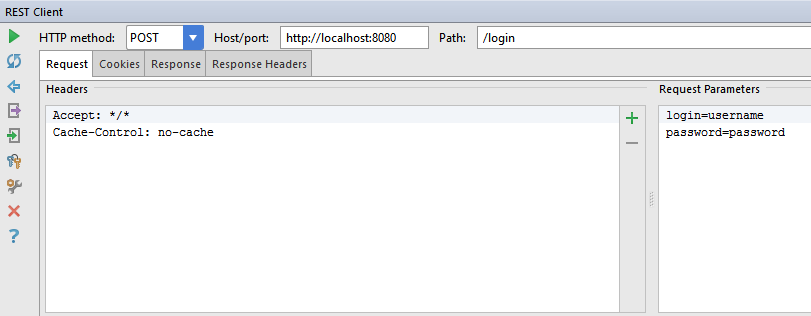
\includegraphics[width=1.0\textwidth, height=1.0\textheight, keepaspectratio ]{img/sekcja3/frontend/logowaniePrzyklad1} }}%
    \qquad
    \subfloat[Odpowiedź na powyższe zapytanie]{{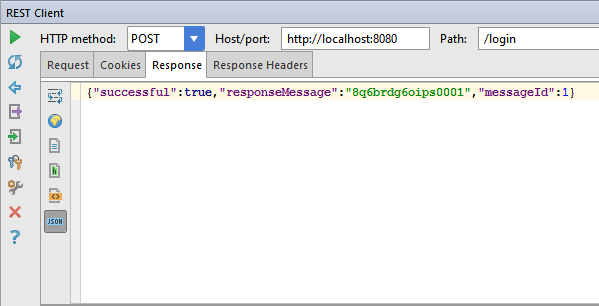
\includegraphics[width=1.0\textwidth, height=1.0\textheight, keepaspectratio]{img/sekcja3/frontend/logowaniePrzyklad2} }}% 
    \caption[Implementacja aplikacji klienckiej - przykładowe zapytanie \textit{HTTP}]{Implementacja aplikacji klienckiej - przykładowe zapytanie \textit{HTTP}}%
\end{figure}

Powyżej widać przykład zapytania generowanego poprzez kod widoczny w poprzednim rysunku, oraz odpowiedź z \textit{serweru backendowego}. Pod polem \textit{"successful"} zapisana jest informacja o powodzeniu zapytania (\textit{true} - powodzenie, \textit{false} - niepowodzenie, a pod \textit{"responseMessage"} widać wygenerowany token dla użytkownika, którym można się teraz posługiwać przy operacjach na indywidualnym koncie, zamiast danych logowania.

%%%%%%%%%%%%%%%%%%%%%%%%%%%%%%%%%%%%%%%%%%%%%%%%%%%%%%%%%%%%%%%%%%%%%%%%
%%%%%%%%%%%%%%%%%%%%%%%%%%%%%%%%%%%%%%%%%%%%%%%%%%%%%%%%%%%%%%%%%%%%%%%%

\subsubsection{Główny moduł aplikacji}\label{Glowny modul aplikacji}
\begin{listing}[H]
\caption[Implementacja aplikacji klienckiej - główny moduł aplikacji]{Implementacja aplikacji klienckiej - główny moduł aplikacji}
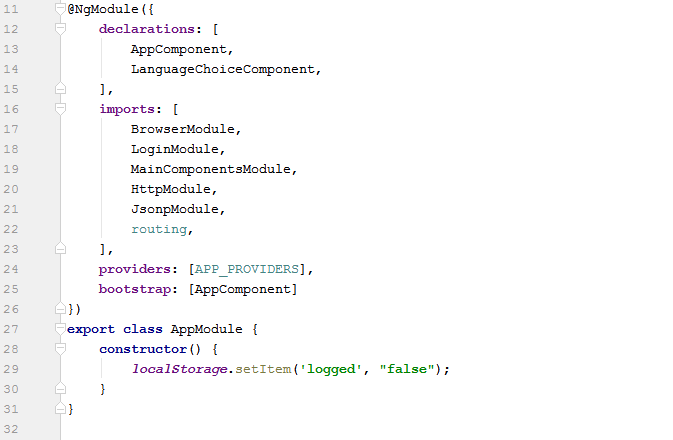
\includegraphics[width=\textwidth]{img/sekcja3/frontend/glownyModulAplikacji}
\end{listing}
Główny moduł aplikacji zawiera wszystkie globalne importowane klasy, oraz inne, zewnętrzne moduły. Poziom importowania (można także importować moduły na niższym poziomie aplikacji), są związane z cyklem życia danego obiektu. Jeśli import zadeklarowany jest na głównym module, to cała aplikacja będzie posiadała jeden obiekt realizujący funkcjonalność importowanej klasy. Ważną deklaracją jest \textit{bootstrap - 25 linia}. Oznacza ona komponent główny, z której rozpocznie się wyświetlanie aplikacji.

\begin{listing}[H]
\caption[Implementacja aplikacji klienckiej - router]{Implementacja aplikacji klienckiej - router}
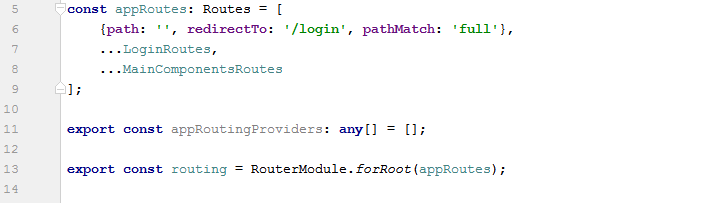
\includegraphics[width=\textwidth]{img/sekcja3/frontend/glowneRoutowanie}
\end{listing}
"Router" jest bardzo ważnym elementem każdej aplikacji internetowy. To on oznacza wszystkie widoczne dla użytkownika \textit{endpointy}, oraz automatyczne przekierowania między nimi. Przykład takiego przekierowania widoczny jest w \textit{6 linii} kodu. Każda próba wejścia na domyślną nazwę strony (\textit{www.nazwastrony.com/}) będzie kończyło się przekierowaniem na podstronę logowania. Poniżej tej linijki dodatkowo są importowane definicje podstron z innych modułów aplikacji.
%%%%%%%%%%%%%%%%%%%%%%%%%%%%%%%%%%%%%%%%%%%%%%%%%%%%%%%%%%%%%%%%%%%%%%%%
%%%%%%%%%%%%%%%%%%%%%%%%%%%%%%%%%%%%%%%%%%%%%%%%%%%%%%%%%%%%%%%%%%%%%%%%

\subsubsection{Logowanie}
Poniżej zaprezentowana jest struktura i kod odpowiedzialny za funkcjonalność logowania i wylogowywania.

\begin{listing}[H]
\caption[Implementacja aplikacji klienckiej - logowanie \textit{HTML}]{Implementacja aplikacji klienckiej - logowanie \textit{HTML}}
\includegraphics[width=1.0\textwidth, height=0.8\textheight]{img/sekcja3/frontend/logowanieHtml}
\end{listing}

Charakterystycznym rozwiązaniem dla języka \textit{Angular2} jest użycie specjalnych znaczników takich jak \textit{*ngIf="warunek" - 1 i 34 linia}. Ten znacznik odpowiada za wyświetlanie danego fragmentu kodu dla użytkownika, przy spełnieniu warunków. Dodatkowo wyświetlane treści przechowywane są w strukturach. Przykład użycia takiej struktury widoczny jest w \textit{ 4, 9, 7 i 27 linii}. Dzięki takiemu rozwiązaniu, bardzo łatwo został zaimplementowany słownik obsługujący wiele języków.

\begin{listing}[H]
\caption[Implementacja aplikacji klienckiej - logowanie \textit{CSS}]{Implementacja aplikacji klienckiej - logowanie \textit{CSS}}
\centering
\includegraphics[scale=0.7]{img/sekcja3/frontend/logowanieCss}
\end{listing}
Powyżej widoczny jest fragment kodu odpowiadający za stylistykę komponentu logowania.

\begin{listing}[H]
\caption[Implementacja aplikacji klienckiej - logowanie \textit{Component}]{Implementacja aplikacji klienckiej - logowanie \textit{Component}}
\includegraphics[width=1.0\textwidth, height=0.8\textheight]{img/sekcja3/frontend/logowanieComponent}
\end{listing}
Powyższy komponent realizuję całą logikę funkcjonalności logowania. Widać na nim charakterystyczną strukturę kodu napisanego w języku \textit{Angular2}. Adnotacja \textit{@Component} oznacza, iż dany element ma być rozpoznawalny jako komponent oraz można go użyć jako znacznik napisany w języku  \textit{HTML - "selector: 'as-login-form" - 10 linia}. Poniżej (\textit{linia 11 oraz 12}) deklarowany jest widok kodu \textit{HTML} wraz z plikiem stylizacji \textit{CSS}, który jest częścią implementacji tego komponentu. Przykładem charakterystycznej funkcji dla \textit{Angular2} jest \textit{ngOnInit - 25 linia} - metoda automatycznie włączająca się za każdym razem gdy użytkownik uruchamia dany komponent (np. poprzez wejście na używającą go podstronę aplikacji).

%%%%%%%%%%%%%%%%%%%%%%%%%%%%%%%%%%%%%%%%%%%%%%%%%%%%%%%%%%%%%%%%%%%%%%%%
%%%%%%%%%%%%%%%%%%%%%%%%%%%%%%%%%%%%%%%%%%%%%%%%%%%%%%%%%%%%%%%%%%%%%%%%

\subsubsection{Widok dostępnych aukcji}
\begin{listing}[H]
\caption[Implementacja aplikacji klienckiej - lista aukcji \textit{HTML}]{Implementacja aplikacji klienckiej - lista aukcji \textit{HTML}}
\includegraphics[width=\textwidth]{img/sekcja3/frontend/listowanieAukcjiHtml}
\end{listing}

Zdjęcie powyżej pokazuje rozwiązanie języka \textit{Angular2} do pokazywania kolekcji. Wystarczy użyć w definicji elementu drzewa \textit{HTML} znacznika \textit{*ngFor="..." - 9 linia kodu} z odpowiednimi argumentami, aby ten element, w zależności od wielkości kolekcji, został wyświetlony. Dodatkowo widać tutaj użycie funkcji, która przekierowuje nas do widoku aukcji po naciśnięciu na odpowiadający jej element.

\begin{listing}[H]
\caption[Implementacja aplikacji klienckiej - lista aukcji \textit{Component}]{Implementacja aplikacji klienckiej - lista aukcji \textit{Component}}
\includegraphics[width=\textwidth]{img/sekcja3/frontend/listowanieAukcjiComponent}
\end{listing}

Widoczny powyżej rysunek przedstawia implementację funkcjonalności i logiki pokazywania aukcji.

%%%%%%%%%%%%%%%%%%%%%%%%%%%%%%%%%%%%%%%%%%%%%%%%%%%%%%%%%%%%%%%%%%%%%%%%
%%%%%%%%%%%%%%%%%%%%%%%%%%%%%%%%%%%%%%%%%%%%%%%%%%%%%%%%%%%%%%%%%%%%%%%%

\subsubsection{Implementacja wielojęzyczności}
Implementacja obsługi wielu języków działa na zasadzie zaczytywania gotowych plików z definicjami wyświetlanego tekstu w schematyczny sposób. Samym zaczytywaniem plików zajmuje się serwis danych, a funkcjonalnością dostępną dla użytkowania odpowiedni komponent.

\begin{listing}[H]
\caption[Implementacja aplikacji klienckiej - implementacja wielojęzyczności - \textit{HTML}]{Implementacja aplikacji klienckiej - implementacja wielojęzyczności - \textit{HTML}}
\includegraphics[width=1.0\textwidth, height=0.17\textheight]{img/sekcja3/frontend/wielojezycznoscHtml}
\end{listing}
Zdjęcie pokazuje napisany kod źródłowy \textit{HTML}. Użytkownik widzi flagi, na które może nacisnąć, aby zmienić wyświetlany język.

\begin{listing}[H]
\caption[Implementacja aplikacji klienckiej - implementacja wielojęzyczności - \textit{CSS}]{Implementacja aplikacji klienckiej - implementacja wielojęzyczności - \textit{CSS}}
\includegraphics[width=\textwidth]{img/sekcja3/frontend/wielojezycznoscCss}
\end{listing}

Powyżej widoczna jest implementacja stylów flag. Po najechaniu myszką na odpowiedni element, jest on otaczany szarym tłem. Kiedy kliknie się na element, zostaje zmieniony kolor obramowania.

\begin{listing}[H]
\caption[Implementacja aplikacji klienckiej - implementacja wielojęzyczności - \textit{Component}]{Implementacja aplikacji klienckiej - implementacja wielojęzyczności - \textit{Component}}
\includegraphics[width=1.0\textwidth, height=0.45\textheight]{img/sekcja3/frontend/wielojezycznoscComponent}
\end{listing}

Serwis \textit{LanguageMessagesReader} odpowiedzialny jest za zaczytywanie odpowiedniego pliku z danymi językowymi. Informacja o aktualnie wyświetlanym języku przechowywana jest w pamięci lokalnej - \textit{localStorage}, za której zmianę odpowiedzialny jest wyżej opisany komponent. Jako argument do głównej metody \textit{readLanguageFile - 13 linia} przyjmuje się nazwę pliku zaczytywanego. Każdy komponent posiada własny plik z definicjami słownika. Następnie zwracany obiekt jest już indywidualnie mapowany na strukturę danych.

\begin{listing}[H]
\caption[Implementacja aplikacji klienckiej - implementacja wielojęzyczności - \textit{Serwis}]{Implementacja aplikacji klienckiej - implementacja wielojęzyczności - \textit{Serwis}}
\includegraphics[width=1.0\textwidth, height=0.35\textheight]{img/sekcja3/frontend/wielojezycznoscSerwis}
\end{listing}

%%%%%%%%%%%%%%%%%%%%%%%%%%%%%%%%%%%%%%%%%%%%%%%%%%%%%%%%%%%%%%%%%%%%%%%%
%%%%%%%%%%%%%%%%%%%%%%%%%%%%%%%%%%%%%%%%%%%%%%%%%%%%%%%%%%%%%%%%%%%%%%%%

\subsubsection{Uruchomienie aplikacji klienckiej}
\begin{figure}[H]
\caption[Wyciąg z konsoli po uruchomienia aplikacji klienckiej]{Wyciąg z konsoli po uruchomienia aplikacji klienckiej}
\includegraphics[width=1.0\textwidth, height=0.8\textheight]{img/sekcja3/frontend/uruchomienieSerwera}
\end{figure}

Powyżej pokazany jest przykład uruchomienia serwera aplikacji klienckiej. Jest on uruchamiany z poziomu linii komend (z katalogu w którym znajduję się plik \textit{index.html}) komendą \textit{npm start}. Kiedy wszystko się załaduję, domyślna przeglądarka internetowa automatycznie włączy się na wyznaczonym adresie aplikacji klienckiej.

%%%%%%%%%%%%%%%%%%%%%%%%%%%%%%%%%%%%%%%%%%%%%%%%%%%%%%%%%%%%%%%%%%%%%%%%
%%%%%%%%%%%%%%%%%%%%%%%%%%%%%%%%%%%%%%%%%%%%%%%%%%%%%%%%%%%%%%%%%%%%%%%%

\newpage
\section{Użytkowanie aplikacji}
Aktualnie aplikacja, dla wygody testowania, posiada widoczny na górze spis wszystkich użytecznych \textit{endpointów}. W przyszłości oczywiście zostanie on wyłączony.
\subsubsection{Logowanie i wylogowywanie}

\begin{figure}[H]
\includegraphics[width=\textwidth]{img/sekcja4/zaloguj}
\caption[Użytkowanie aplikacji - logowanie]{Użytkowanie aplikacji - logowanie}
\end{figure}

\begin{figure}[H]
\includegraphics[width=\textwidth]{img/sekcja4/wyloguj}
\caption[Użytkowanie aplikacji - wylogowanie]{Użytkowanie aplikacji - wylogowanie}
\end{figure}

Powyższe dwa rysunki przedstawiają funkcjonalność logowania i wylogowywania. Aby zalogować się, użytkownik musi podać nazwę użytkownika, bądź adres e-mail, użyty przy rejestracji konta.

\subsubsection{Stworzenie nowej aukcji}

\begin{figure}[H]
\includegraphics[width=\textwidth]{img/sekcja4/stworzenieNowejAukcji}
\caption[Użytkowanie aplikacji - stworzenie nowej aukcji]{Użytkowanie aplikacji - stworzenie nowej aukcji}
\end{figure}

Wszystkie pola aukcji muszą być wypełnione. W innym przypadku nowa aukcja nie zostanie zapisana do bazy danych. Dodatkowo, aby można było stworzyć aukcję, użytkownik musi być zalogowany.

\subsubsection{Stworzenie nowego użytkownika}
\begin{figure}[H]
\includegraphics[width=\textwidth]{img/sekcja4/stworzenieNowegoUzytkownika}
\caption[Użytkowanie aplikacji - stworzenie nowego użytkownika]{Użytkowanie aplikacji - stworzenie nowego użytkownika}
\end{figure}
Użytkownik musi wprowadzić prawidłowy adres e-mail, aby stworzenie konta powiodło się.

\begin{figure}[H]
\includegraphics[width=\textwidth]{img/sekcja4/przykladowyEmail}
\caption[Użytkowanie aplikacji - aktywacja nowego użytkownika]{Użytkowanie aplikacji - aktywacja nowego użytkownika}
\end{figure}
Jest to przykładowy e-mail wysłany po rejestracji konta. Użytkownik musi jedynie kliknąć w link aktywacyjny.

\subsubsection{Wyświetlenie aukcji}
\begin{figure}[H]
\includegraphics[width=\textwidth]{img/sekcja4/listowanieAukcji}
\caption[Użytkowanie aplikacji - wyświetlanie aukcji]{Użytkowanie aplikacji - wyświetlanie aukcji}
\end{figure}

Podstawowe wyświetlanie aukcji (na razie bez funkcjonalności wyszukiwania interesujących nas rekordów przy użyciu parametrów). Użytkownik może nacisnąć na wybrany wiersz, reprezentujący interesującą go aukcję, aby przejść do widoku poszczególnej aukcji. Dodatkowo po prawej stronie widoczne są flagi umożliwiające zmianę wyświetlanego języka.

\begin{figure}[H]
\includegraphics[width=\textwidth]{img/sekcja4/wygladAukcji}
\caption[Użytkowanie aplikacji - wyświetlenie konkretnej aukcji]{Użytkowanie aplikacji - wyświetlenie konkretnej aukcji}
\end{figure}

Jedynie funkcjonalność przejścia na konkretną podstronę została zaimplementowana, widok ma za zadanie potwierdzić poprawną integrację środowiska. Na samej górze widać pasek adresu, cyfra jest dynamicznie przetwarzana i odpowiadająca jej aukcja wyświetlana.

%%%%%%%%%%%%%%%%%%%%%%%%%%%%%%%%%%%%%%%%%%%%%%%%%%%%%%%%%%%%%%%%%%%%%%%%
%%%%%%%%%%%%%%%%%%%%%%%%%%%%%%%%%%%%%%%%%%%%%%%%%%%%%%%%%%%%%%%%%%%%%%%
\newpage
\section{Wdrożenie i ocena jakości}
\subsection{Podstawowe wymagania instalacji systemu}\label{Podstawowe wymagania instalacji systemu}
\subsubsection{Instalacja Javy}
\paragraph{Instalacja dla systemu Windows}
Należy pobrać najnowszy pakiet Javy z oficjalnej dystrybucji Oracle (\underline{min. JDK/JRE 1.8.97}) i zainstalować go:
http://www.oracle.com/technetwork/java/javase/downloads/index.html
\paragraph{Instalacja dla Linuxa Ubuntu}
Domyślnie do każdego systemu Ubuntu dołączany jest pakiet JDK javy. Do uruchomienia aplikacji potrzebna jest pakiet \underline{JDK/JRE 1.8.97} lub wyższy.
Te wymagania spełnia chociażby najnowsza wersja Ubuntu 16.06

%%%%%%%%%%%%%%%%%%%%%%%%%%%%%%%%%%%%%%%%%%%%%%%%%%%%%%%%%%%%%%%%%%%%%%%%
%%%%%%%%%%%%%%%%%%%%%%%%%%%%%%%%%%%%%%%%%%%%%%%%%%%%%%%%%%%%%%%%%%%%%%%%

\subsubsection{Instalacja Maven'a}
Dla obydwu systemów:
Należy postępować zgodnie z instrukcją, która znajduje się na stronie głównej po kliknięciu na "Download", a następnie "Install". Instrukcje "Run" należy pominąć.
https://maven.apache.org/

%%%%%%%%%%%%%%%%%%%%%%%%%%%%%%%%%%%%%%%%%%%%%%%%%%%%%%%%%%%%%%%%%%%%%%%%
%%%%%%%%%%%%%%%%%%%%%%%%%%%%%%%%%%%%%%%%%%%%%%%%%%%%%%%%%%%%%%%%%%%%%%%%

\subsubsection{Instalacja nodeJS}
\paragraph{Instalacja dla systemu Windows}
Sciągamy odpowiednią wersję pliku instalacyjnego ze strony:
https://nodejs.org/en/download/
i postępujemy wg. instrukcji.
Po instalacji wykonanie komendy \textit{npm -v} w wierszu poleceń powinno zwrócić wersję.
\paragraph{Instalacja dla Linuxa Ubuntu}
Wykonujemy serię poleceń z linii komend
\begin{enumerate}[1.]
\item \textit{sudo apt-get update}
\item \textit{sudo apt-get install nodejs}
\item \textit{sudo apt-get install npm}
\item Jeśli wszystko przebiegło pomyślnie to komenda: \textit{npm --version} powinna zwrócić aktualną wersję
\end{enumerate}

%%%%%%%%%%%%%%%%%%%%%%%%%%%%%%%%%%%%%%%%%%%%%%%%%%%%%%%%%%%%%%%%%%%%%%%%
%%%%%%%%%%%%%%%%%%%%%%%%%%%%%%%%%%%%%%%%%%%%%%%%%%%%%%%%%%%%%%%%%%%%%%%%

\subsubsection{Instalacja i konfiguracja bazy danych}
\paragraph{Instalacja dla systemu Windows}
Na tym systemie instalacja sprowadza się do ściągnięcia najnowszej paczki instalacyjnej \textit{.msi} ze strony: \href{https://dev.mysql.com/downloads/mysql/}{https://dev.mysql.com/downloads/mysql/}
Następnie należy przejść do instalacji. Nie należy zmieniać domyślnych ustawień podczas instalacji.

\paragraph{Za każdym uruchomieniem serwera należy uruchomić serwis bazodanowy:}  
\begin{enumerate}[a.]
\item Włączamy wyszukiwarkę \textit{Windows}.
\item W wyszukiwarce wpisujemy: \textit{usługi} bądź \textit{services}.
\item Wyszukujemy serwis MySQL i klikamy na niego prawym klawiszem myszki.
\item Wybieramy opcję \textit{uruchom}.
\end{enumerate}

\paragraph{Instalacja dla Linuxa Ubuntu}
W systemie \textit{Ubuntu} instalacja \textit{MySQL} sprowadza się do wpisania jednej komendy. Należy wpisać polecenie:
	sudo apt-get install mysql-server
Nasępnie należy postępować zgodnie z instrukcją.

\paragraph{Aby uruchomić serwis bazodanowy należy:}
\begin{enumerate}[1.]
\item Włączyć konsolę oraz wpisać komendę: \textit{service --status-all}
\item Następnie znaleźć nasz serwis bazodanowy, domyślnie \textit{MySQL}
\item Wyszukaną nazwę należy podać w komendzie \textit{service <service name> start}
		przykład: service MySQL start
\end{enumerate}


\paragraph{(Linux i Windows) Konfiguracja bazy danych} 
\begin{enumerate}[1.]
\item Za pomocą polecenia należy zalogować się do bazy \textit{MySQL} poleceniem:
		\textit{mysql -u root -p}
\item Następnie należy wpisać hasło i zaakceptować
\item Stwórz bazę danych poleceniem: 
		\textit{create database \textless nazwa\_bazy\_danych \textgreater;}
\item Wybierz utworzoną bazę danych za pomocą komendy:
		\textit{use \textless nazwa\_bazy\_danych \textgreater;}
\item Załaduj plik tworzący bazę danych:
		\textit{source \textless scieżka\_do\_pliku \textgreater;}

		\textless nazwa\_bazy\_danych \textgreater , przykład: db
		
		\textless scieżka\_do\_pliku \textgreater , przykład: C:/user/Adam/Desktop/bazadanych.sql
		
\end{enumerate}

%%%%%%%%%%%%%%%%%%%%%%%%%%%%%%%%%%%%%%%%%%%%%%%%%%%%%%%%%%%%%%%%%%%%%%%%
%%%%%%%%%%%%%%%%%%%%%%%%%%%%%%%%%%%%%%%%%%%%%%%%%%%%%%%%%%%%%%%%%%%%%%%%

\subsection{Instalacja i budowa aplikacji}\label{Instalacja i budowa aplikacji}
Aby przystąpić do uruchomienia aplikacji, należy najpierw przejść przez etap instalacji narzędzi - \ref{Podstawowe wymagania instalacji systemu}.
\begin{enumerate}[1.]
\item Należy ściągnąć ze strony i rozpakować projekt do folderu np. C:/projekt 

\subparagraph{Ręczne ściągnięcie}\mbox\\

Należy wejść na stronę oraz ściągnąć projekt w formacie .zip
\href{https://bitbucket.org/holkiew/applicationnamegamma}{https://bitbucket.org/holkiew/applicationnamegamma}

\subparagraph{Ściągnięcie za pomocą systemu \textit{Git}}
Link który należy podać przy tworzeniu nowego lokalnego repozytorium
\textit{https://holkiew@bitbucket.org/holkiew/applicationnamegamma.git}
\item Wejść do katalogu w którym rozpakowaliśmy projekt (\underline{upewnić się, że jest w nim plik pom.xml}, jeśli go nie ma, wyszukać go i przejść do tego katalogu)
\item Uruchomić linię komend (np. wpisując w domyślnym eksploratorze Windows, w miejscu gdzie jest widoczna ścieżka do katalogu, \textit{cmd})
\item W okienku wiersza poleceń wpisujemy: \textit{mvn clean install}
\item Po pomyślnej instalacji wpisujemy \textit{mvn build}
\item Następnie wchodzimy do katalogu "target", np. C:/projekt/target i wyszukujemy plik \textit{projekt-numerWersji-SNAPSHOT.jar} np. \textit{projekt-0.0.1-SNAPSHOT.jar}
\item Upewniamy się czy plik jest aktualny (Data modyfikacji pliku)
\item Wchodzimy do katalogu \textit{frontend} np. \textit{C:/projekt/frontend}
\item Uruchamiamy linię komend w tym katalogu
\item Wpisujemy komendę \textit{npm install} (instalacja trwa około 2 minuty)
\end{enumerate}

%%%%%%%%%%%%%%%%%%%%%%%%%%%%%%%%%%%%%%%%%%%%%%%%%%%%%%%%%%%%%%%%%%%%%%%%
%%%%%%%%%%%%%%%%%%%%%%%%%%%%%%%%%%%%%%%%%%%%%%%%%%%%%%%%%%%%%%%%%%%%%%%%

\subsection{Uruchomienie aplikacji}
Jeśli dostarczony został kod źródłowy aplikacji, należy uprzednio wykonać kroki z działu \ref{Instalacja i budowa aplikacji}.
\begin{enumerate}[1.]
\item Uruchamiamy serwis bazy danych
\item Wyszukujemy plik aplikacji (np. \textit{projekt-0.0.1-SNAPSHOT.jar})
\item Wchodzimy do tego pliku np. za pomocą programu \textit{WinRAR} (otwórz za pomocą WinRAR) bądź innego programu do archiwizacji danych
\item Przechodzimy do katalogu \textit{BOOT-INF/classes/}
\item Konfigurujemy odpowiednie pliki, gdzie:
\begin{enumerate}[A.]
\item \textit{application.properties} - zmieniamy tylko namiary na bazę danych (port oraz dane logowania)
\item \textit{hibernate-annotation.cfg.xml} - robimy to samo co powyżej
\item \textit{mail.properties} zmieniamy konfiguracje serwisu poczty elektronicznej z której będzie korzystać aplikacja
\item \textit{web.properties} zmieniamy właściwości aplikacji
\end{enumerate}
\item Uruchamiamy aplikację (podwójne kliknięcie na plik \textit{.jar} np. \textit{projekt-0.0.1-SNAPSHOT.jar})
\item Wchodzimy do katalogu gdzie znajduje się aplikacja kliencka (domyślnie katalog \textit{frontend})
\item Plik w katalogu \textit{frontend/src/config/gulp/config.js} zawiera konfigurację portów wyjściowych
\item Uruchamiamy linię komend i wpisujemy komendę: \textit{npm run serve-build} co uruchamia serwer aplikacji
\item *Jeśli chcemy wygenerować tylko pliki statyczne, aby uruchomić stronę na własnym serwerze, należy użyć komendy \textit{npm run build} zamiast \sout{\textit{npm run serve-build}}. Będą one znajdować się w katalogu \textit{frontend/build}
\end{enumerate}
\subsection{Testy aplikacji}
Rozdział ten został podzielony na dwa podrozdziały. W pierwszym z nich zostały omówione testy które już istnieją w systemie. W drugim natomiast są opisane testy które należy stworzyć. Testy automatyczne są napisane jedynie na poziomie serwera aplikacji. Strona kliencka była testowana ręcznie.
\subsubsection{Istniejące testy}
Zostały stworzone testy jednostkowe polegające na sprawdzaniu przy każdym uruchomieniu serwera czy żaden z kontrolerów nie zmienił swojej definicji (przyjmowanych parametrów, rodzaju zapytania \textit{HTTP}) oraz zwracanego obiektu. Do stworzenia tych testów została użyta biblioteka \textit{Mockito} umożliwiająca zaślepienie funkcjonalności pobierania informacji z bazy danych. Są to bardzo ważne testy, ponieważ każda zmiana definicji \textit{endpointa} może popsuć wymianę informacji z aplikacjami klienckimi.
\subsubsection{Testy które powinny zostać zaimplementowane}
\begin{enumerate}[1.]
\item Testy jednostkowe funkcji logicznych serwera jak i aplikacji klienckiej.
\item Testy \textit{endpointów} aplikacji klienckiej.
\item Testy tzw. \textit{End-to-end}, polegające na przetestowaniu całej ścieżki konkretnej funkcjonalności aplikacji, np. tworzenia aukcji. 
\item Testy integracyjne sprawdzające połączenia pomiędzy poszczególnymi modułami systemu.
\item Testy sprawdzające "wytrzymałość" aplikacji polegające na generowaniu losowych akcji przez określony czas na aplikacji klienckiej. Takie testy pomogłyby znaleźć nietypowe, trudne do wykrycia błędy.
\end{enumerate}
\subsection{Weryfikacja}
System napisany jest bez wewnętrznej dokumentacji, jednakże wystarczającymi opisami są nazwy klas oraz ich funkcjonalność. Jest to spełnienie jednego z wymagań niefunkcjonalnych. 
Rozwiązania podzielone są na jak największą ilość metod, które opisują słownie, krok po kroku, implementacje funkcjonalności. Każdy powtórzony kod (np. jedna pętla zmieniająca dane, używana w ten sam sposób przez wiele innych metod) jest opakowany w funkcję. Takie rozwiązanie umożliwia łatwe wykrycie oraz naprawę błędów (które w innym przypadku, nawet po wykryciu, byłyby bardzo czasochłonne do wykrycia). Dodatkowo system został oparty na dobrze znanym wzorcu projektowym \textit{MVC - Model-View-Controller}. Każda oddzielna funkcjonalność aplikacji posiada swój własny pakiet w projekcie. Podejście takie umożliwia łatwą segregację kodu oraz utrzymuje porządek i ułatwia poruszanie się po aplikacji. Stworzone i zaprojektowane testy pomagają nie tylko szybko wychwytywać błędy w oprogramowaniu jak i komunikacji pomiędzy poszczególnymi modułami, ale także służą do informowania osób modyfikujących kod, że ich zmiana może istotnie wpłynąć na inne funkcjonalności systemu. Dodatkowo zostały wykonane testy sprawdzające działanie aplikacji klienckiej na najpopularniejszych przeglądarkach internetowych - \textit{Mozilla Firefox, Google Chrome, Microsoft Internet Explorer}. Na wszystkich z nich aplikacja działała poprawnie.
\subsection{Walidacja}
Na tym poziomie projektu bardzo trudno jest ocenić czy system jest prawidłowy ponieważ do jego funkcjonowania potrzebna jest dobrze zrealizowana aplikacja kliencka, współdziałająca z serwerem oraz bazą danych. O ile baza danych jest dobrze zaprojektowana i spełnia swoje zadania o tyle serwer jak i aplikacja kliencka jeszcze tego nie robią. Należałoby poświęcić jeszcze dużo czasu nad implementacją tych dwóch modułów systemu, aby doprowadzić je do pełnej używalności. Wtedy można byłoby ocenić poprawność systemu, jednakże na ten moment stworzony system nie spełnia wszystkich założeń.
%%%%%%%%%%%%%%%%%%%%%%%%%%%%%%%%%%%%%%%%%%%%%%%%%%%%%%%%%%%%%%%%%%%%%%%%
%%%%%%%%%%%%%%%%%%%%%%%%%%%%%%%%%%%%%%%%%%%%%%%%%%%%%%%%%%%%%%%%%%%%%%%%

\newpage
\section{Podsumowanie}
\subsection{Technologie}\label{Technologie}
Jednym z celów pracy była nauka nowych technologii. Poniżej streściłem swoją subiektywną opinię nad głównie używanymi narzędziami przy tworzeniu pracy dyplomowej. 
Wszystkie użyte technologie, stojące po stronie \textit{serwera backendowego}, czyli \textit{Spring} oraz \textit{Hibernate} okazały się bardzo dobrym wyborem. Są one dobrze udokumentowane, oficjalnie jak i nieoficjalnie, poprzez wsparcie przez innych użytkowników na forach. Nie doszukałem się żadnych błędów wymagających ode mnie zmiany podejścia do implementacji kodu. Baza danych postawiona przy użyciu \textit{MySQL}, także nie sprawiała żadnych problemów. Jednakże dużo czasu spędziłem na konfiguracji aplikacji. Pomimo tego uważam, że czas poświęcony na to był optymalny do rozmiaru mojego projektu, ponieważ kiedy miałem napisane już wszystkie "szablony", tworzenie widocznej i użytkowej funkcjonalności zajmowało porównywalnie mało czasu do implementacji bez użycia tych dwóch technologii. \mbox{}\\
Niestety zawiodłem się na wybranej przeze mnie technologii realizująca widok u klienta czyli \textit{Angular2}. Kiedy zaczynałem konfigurować projekt, technologia była jeszcze w fazie \textit{Alfa}, jednakże z wyczytanych opinii innych użytkowników wywnioskowałem, iż jest na tyle stabilna, aby spróbować przy jej użyciu napisać aplikację kliencką. Niestety po miesiącu do użytku trafiła wersja finalna, która znacznie zmieniła podejście do deklaracji poszczególnych komponentów tworzących aplikację, jak i same krytyczne komponenty użytkowe (np. router) czy sposób uruchomienia głównego modułu. Wraz z tymi zmianami, większość bibliotek stworzonych przez indywidualnych użytkowników, jak i wszelakich wskazówek i rozwiązań popularnych problemów, dostępnych na forach, przestały być kompatybilne z aktualną wersją języka. Z początku było to dla mnie, początkującego użytkownika tego języka jak i rejonu technologii aplikacji internetowych, bardzo uciążliwe i mylące. Sama ta zmiana wymusiła na mnie przepisanie mojego kodu, co skutkowało straceniem około jednego dnia, na zrozumienie nowego podejścia i doprowadzenie mojej aplikacji do stanu użytkowego. Dodatkowo kiedy chciałem użyć biblioteki napisanej przez innego użytkownika, implementującą funkcjonalność \textit{Google Maps}, okazało się, że została ona napisana właśnie za czasów wersji \textit{Angular2 Alfa} i nie jest kompatybilna. Kolejnym problemem jest słabo opisana oficjalna dokumentacja oraz system \textit{deploymentu} aplikacji. Dopiero od wersji finalnej \textit{Angular2}, twórcy zaczeli wspierać oficjalne narzędzie kontroli i konfiguracji projektu - \href{https://cli.angular.io/}{\textit{Angular CLI}}. Niestety nie jest one perfekcyjne, bardzo dużo problemów jest z stworzeniem wersji produkcyjnej. Mimo wszystko uważam, iż jest to przyszłościowa technologia i jeśli jej twórcy rozwiążą większość aktualnych problemów, nowi użytkownicy chętniej sami zaczną ją wspierać poprzez własne rozszerzenia jak i obszerne informacje zwrotne.

\subsection{Realizacja pracy}

Realizacja pracy niestety nie przebiegła według założonego harmonogramu. Powodem tego było przecenienie własnej wytrzymałości. Założyłem, iż po każdym pełnym dniu pracy, przez 2 do 4 godzin będę pracować na pracą dyplomową. Pisanie aplikacji w taki sposób było bardzo nieefektywne, ponieważ byłem już zazwyczaj zmęczony całodniowym siedzeniem przed monitorem. Finalnie skończyło się na pisaniu pracy dyplomowej tylko w weekendy i to nie każde ze względu na liczne wyjazdy.\mbox{}\\
Implementacja aplikacji pokazała, że nie wolno lekceważyć nowych technologii. Próg wejściowy do \textit{Angulara2} dla człowieka który nic nie miał wspólnego z technologiami webowymi jest na tyle duży, że musiałem kompletnie pominąć realizację samego wyglądu dla użytkownika. \textit{Framework} \textit{Hibernate} także przysporzył wiele problemów związanych z niezrozumieniem działania tej technologii, co znacznie opóźniło skonfigurowanie bazy danych w kodzie \textit{Java}. Do ostatniego założonego dnia harmonogramu, udało mi się zrealizować projekt systemu, analizę rynku i technologii oraz część implementacji aplikacji. Po tym terminie dodatkowo udało mi się zrealizować funkcjonalność wielojęzyczności, testy po stronie serwera jak i dokończenie pisania pracy dyplomowej.\mbox{}\\
Podsumowując, wszystkie założone, główne cele projektu czyli \textit{porównanie istniejących rozwiązań}, \textit{analiza dostępnych narzędzi}, \textit{zaprojektowanie systemu realizującego funkcjonalność tematu pracy dyplomowej} i textit{zaprojektowanie bazy danych} zostały spełnione. Cel opisany jako \textit{nauka nowych technologii} został podsumowany w rozdziale - \hyperref[Technologie]{Technologie}. \mbox{}\\
Z dodatkowych celów jedynie \textit{implementacja wielojęzyczności aplikacji} została stworzona. Drugi z dodatkowych celów czyli \textit{stworzenie dodatkowego interfejsu użytkownika na telefony komórkowe} okazał się zbyt czasochłonny, aby nawet rozpocząć jego projektowanie.

\subsection{Wnioski}

Dzięki projektowi nauczyłem się nowego podejścia do programowania - webowego oraz najpopularniejszego wzorca projektowego aplikacji internetowych \textit{MVC - Model View Controller} jak i nowoczesnych, cenionych na rynku pracy, technologii i narzędzi umożliwiających szybką pracę w tej dziedzinie informatyki.\mbox\\
Jednakże nie tylko miałem zaimplementować aplikację, ale też ją zaprojektować, łącznie z analizą rynku jak i technologiczną. Faza ta jest bardzo wymagająca i czasochłonna. Dobry projekt znacznie skraca czas implementacji oraz ucina wiele niepotrzebnych dyskusji nad funkcjonalnością do zaimplementowania, która może być postrzegana przez wielu ludzi inaczej, jeśli nie jest opisana, bądź jest opisana, ale niejasno i niejednoznacznie.
Rozwój aplikacji będzie kontynuowany.

\subsection{Dalsze możliwości rozwoju systemu}
Projektowana aplikacja jest za duża, aby w proponowanym czasie ją kompletnie rozwiązać. Jest to zadanie na więcej osób, co wiąże się z kosztami, jak i wymaganymi później dochodami, aby ją utrzymać. Możliwości i cele przyszłego rozwoju aplikacji są następujące
\begin{enumerate}[1.]
\item Reklama aplikacji w serwisach internetowych pokrewnych z tematyką transportu towarów oraz w popularnych serwisach aukcyjnych np. \textit{Allegro}
\item Zachęcenie dużych firm poprzez wprowadzenie dodatkowej funkcjonalności wspomagającej obsługę wielu zleceń i osób do zarządzania.
\item Pozyskanie funduszy na dalszy rozwój aplikacji np. unijnych bądź prywatnych inwestorów.
\item Stworzenie tzw. \textit{Start-up'u}.
\end{enumerate}

%%%%%%%%%%%%%%%%%%%%%%%%%%%%%%%%%%%%%%%%%%%%%%%%%%%%%%%%%%%%%%%%%%%%%%%%
%%%%%%%%%%%%%%%%%%%%%%%%%%%%%%%%%%%%%%%%%%%%%%%%%%%%%%%%%%%%%%%%%%%%%%%%
\mbox{}
\thispagestyle{empty}
\newpage


%%%%%%%%%%%%%%%%%%%%%%%%%%%%%%%%%%%%%%%%%%%%%%%%%%%%%%%%%%%%%%%%%%%%%%%%%%%%%%
%%%%%%%%%%%%%%%%%%%%%%%%%%%%%%% BIBLIOGRAFIA %%%%%%%%%%%%%%%%%%%%%%%%%%%%%%%%%
%%%%%%%%%%%%%%%%%%%%%%%%%%%%%%%%%%%%%%%%%%%%%%%%%%%%%%%%%%%%%%%%%%%%%%%%%%%%%%
\addcontentsline{toc}{section}{Literatura}
\bibliographystyle{plain}
\bibliography{P2P}

\mbox{}
\thispagestyle{empty}
\newpage

\appendix
\section{Opis załączonej płyty CD/DVD}
\begin{enumerate}[$\bullet$]
\item Katalog \textit{projekt} - zawiera cały projekt (aplikacja serwerowa jak i kliencka). Można go zainstalować na każdym środowisku, pamiętając o uprzedniej instalacji \textit{Maven'a} który zarządza zależnościami. Użyte \textit{IDE} do pisaniu projektu: \textit{IntelliJ IDEA 15.0.4} - program ten nie powinien mieć żadnych kłopotów z instalacją projektu.
\item Katalog \textit{bin} - zawiera, skompilowany, plik wykonywalny \underline{samego} serwera \textit{backendowego} (należy odpowiednio skonfigurować bazę danych) oraz zbudowane pliki aplikacji klienckiej.
\item Katalog \textit{app\_src} - zawiera pełne kody źródłowe plików pokazanych w pracy dyplomowej (listingi). 
\item Katalog \textit{pdyp\_src} - zawiera wszystkie pliki źródłowe pisanej pracy dyplomowej (wraz z samą pracą).
\item Katalog \textit{img} - zawiera widoki obrazujące działanie systemu.
\end{enumerate}
\end{document}
